	\section{Eje Z}
	\subsection{Material necesario}
		\begin{itemize}
			\item Piezas impresas Base y Z Coupling
			\item 8x tornillo M3x15
			\item 6x tornillos M3x10.
			\item Bridas.
			\item 24x tuercas M8.
			\item 10x arandelas M8.
			\item 4x rodamientos lineales LM8UU.
			\item 2x rodamientos axiales 608 zz blindados.
			\item 4x varillas roscadas M8x320.
			\item 2x varillas lisas M8x340.
			\item Correa T2.5 de 615mm.
			\item 2x tornillos M3x30.
			\item 10x tuercas M3.

		\end{itemize}
		\begin{figure}[!htp]
			\centering
			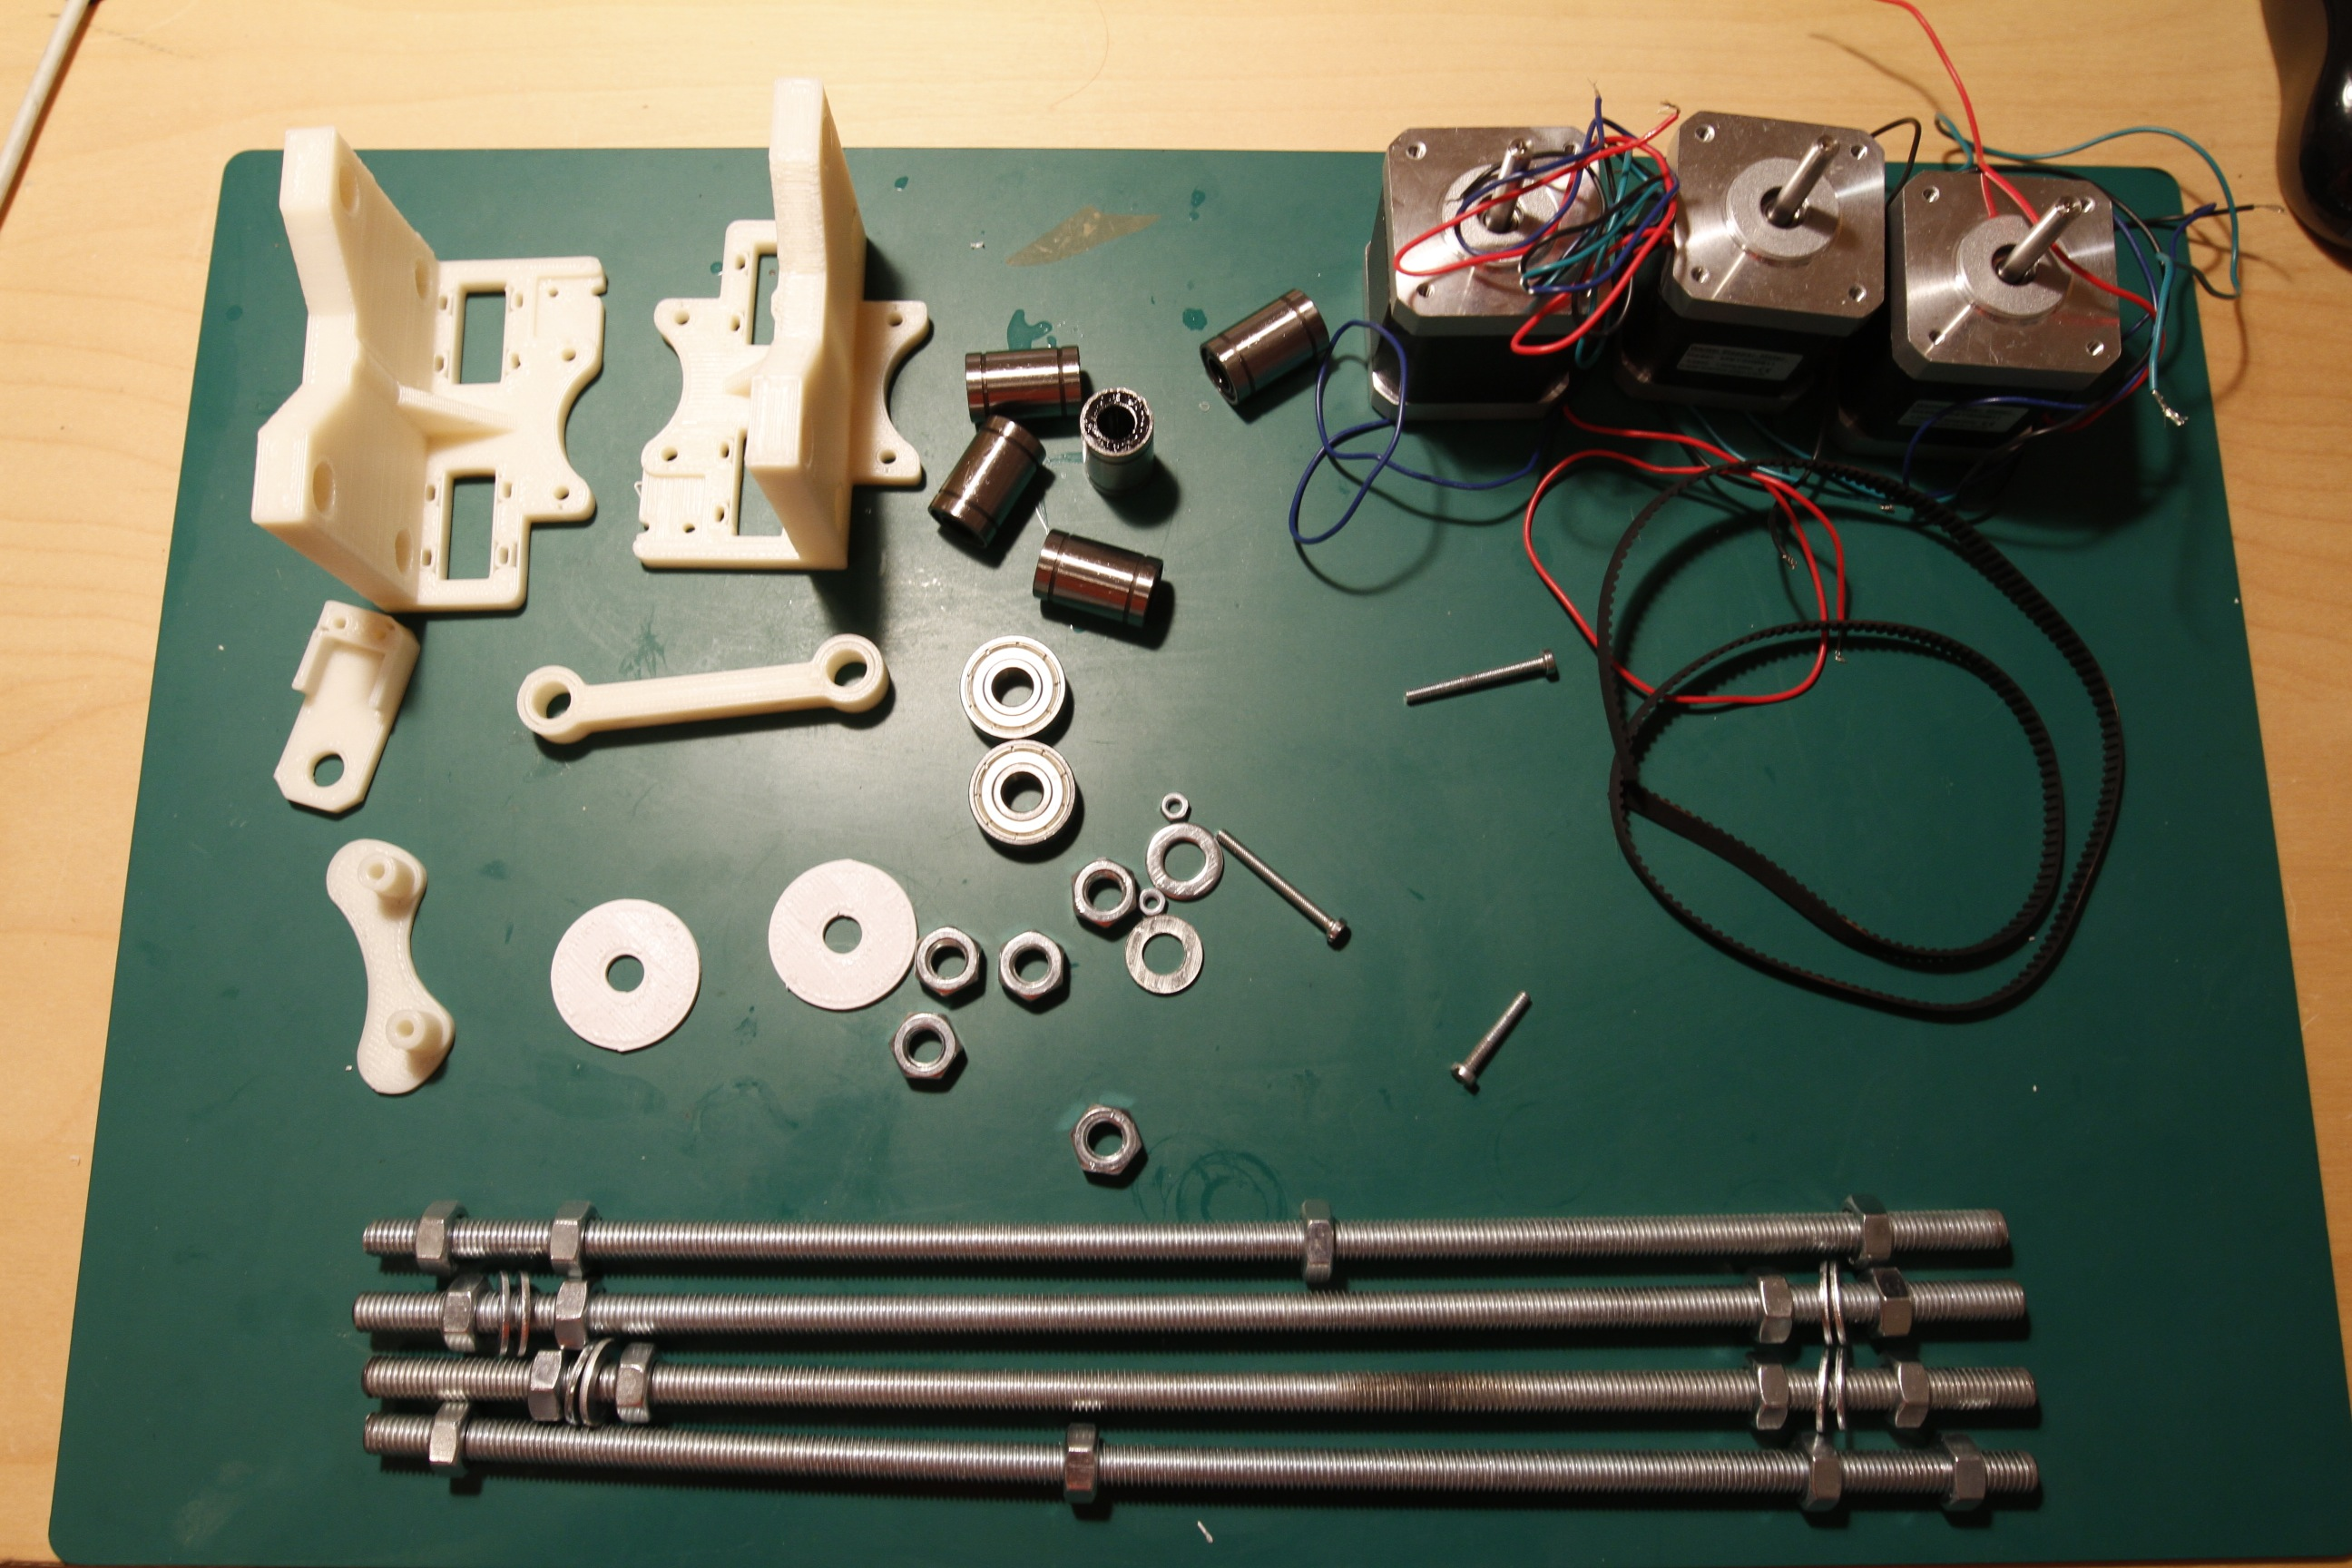
\includegraphics[width=0.7\textwidth]{../../Fotos/67.jpg}
			\caption{Material necesario}
		\end{figure}
		\newpage{}
	\subsection{Herramienta necesaria}
		\begin{itemize}
			\item Alicates de punta fina.
			\item Alicates de corte o tijeras.
			\item Destornillador.
			\item Llave inglesa para M8.
			\item Cinta métrica.
			\item Destornilladores.
			\item Soldador.
			\item Lima fina.
		\end{itemize}
		\begin{figure}[!htp]
			\centering
			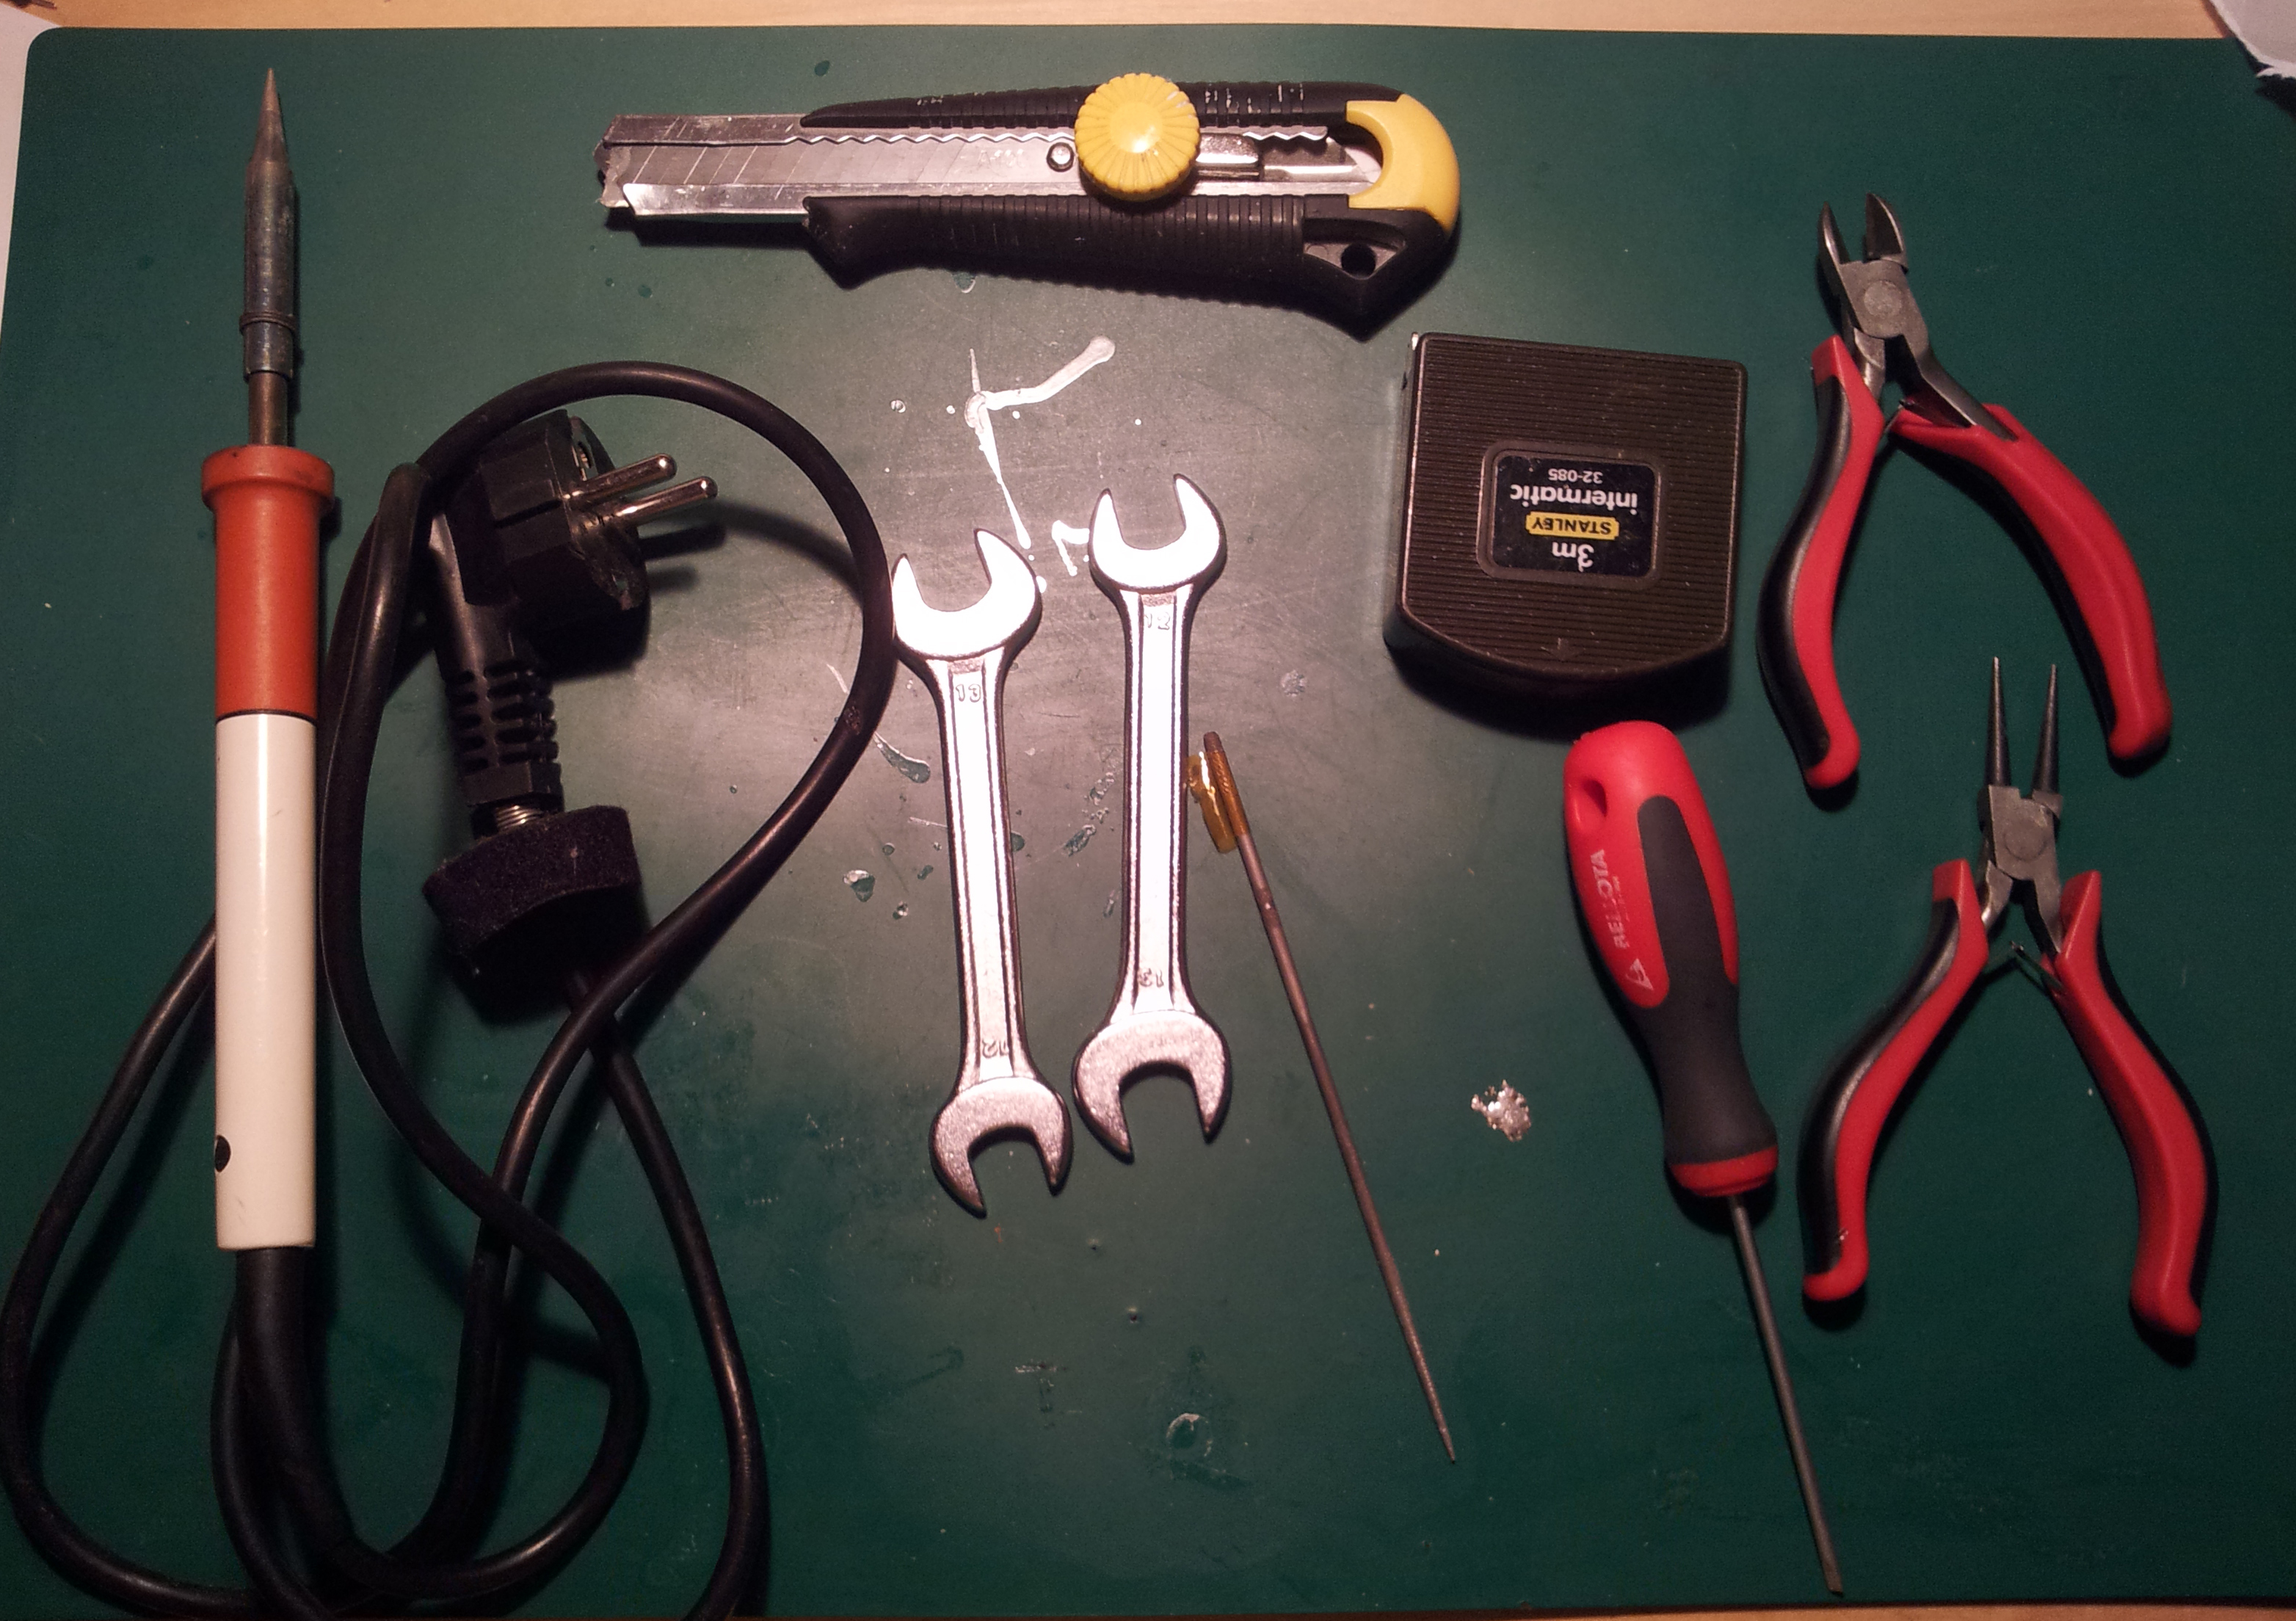
\includegraphics[width=0.7\textwidth]{../../Fotos/67b.jpg}
			\caption{Herramienta necesaria}
		\end{figure}
		\newpage{}
			\subsection{Operativa}
		Empezaremos montando la base introduciendo cuatro varillas roscadas con tuercas y arandelas como se muestran en las fotos a continuación:
		\begin{figure}[!htp]
			\centering
			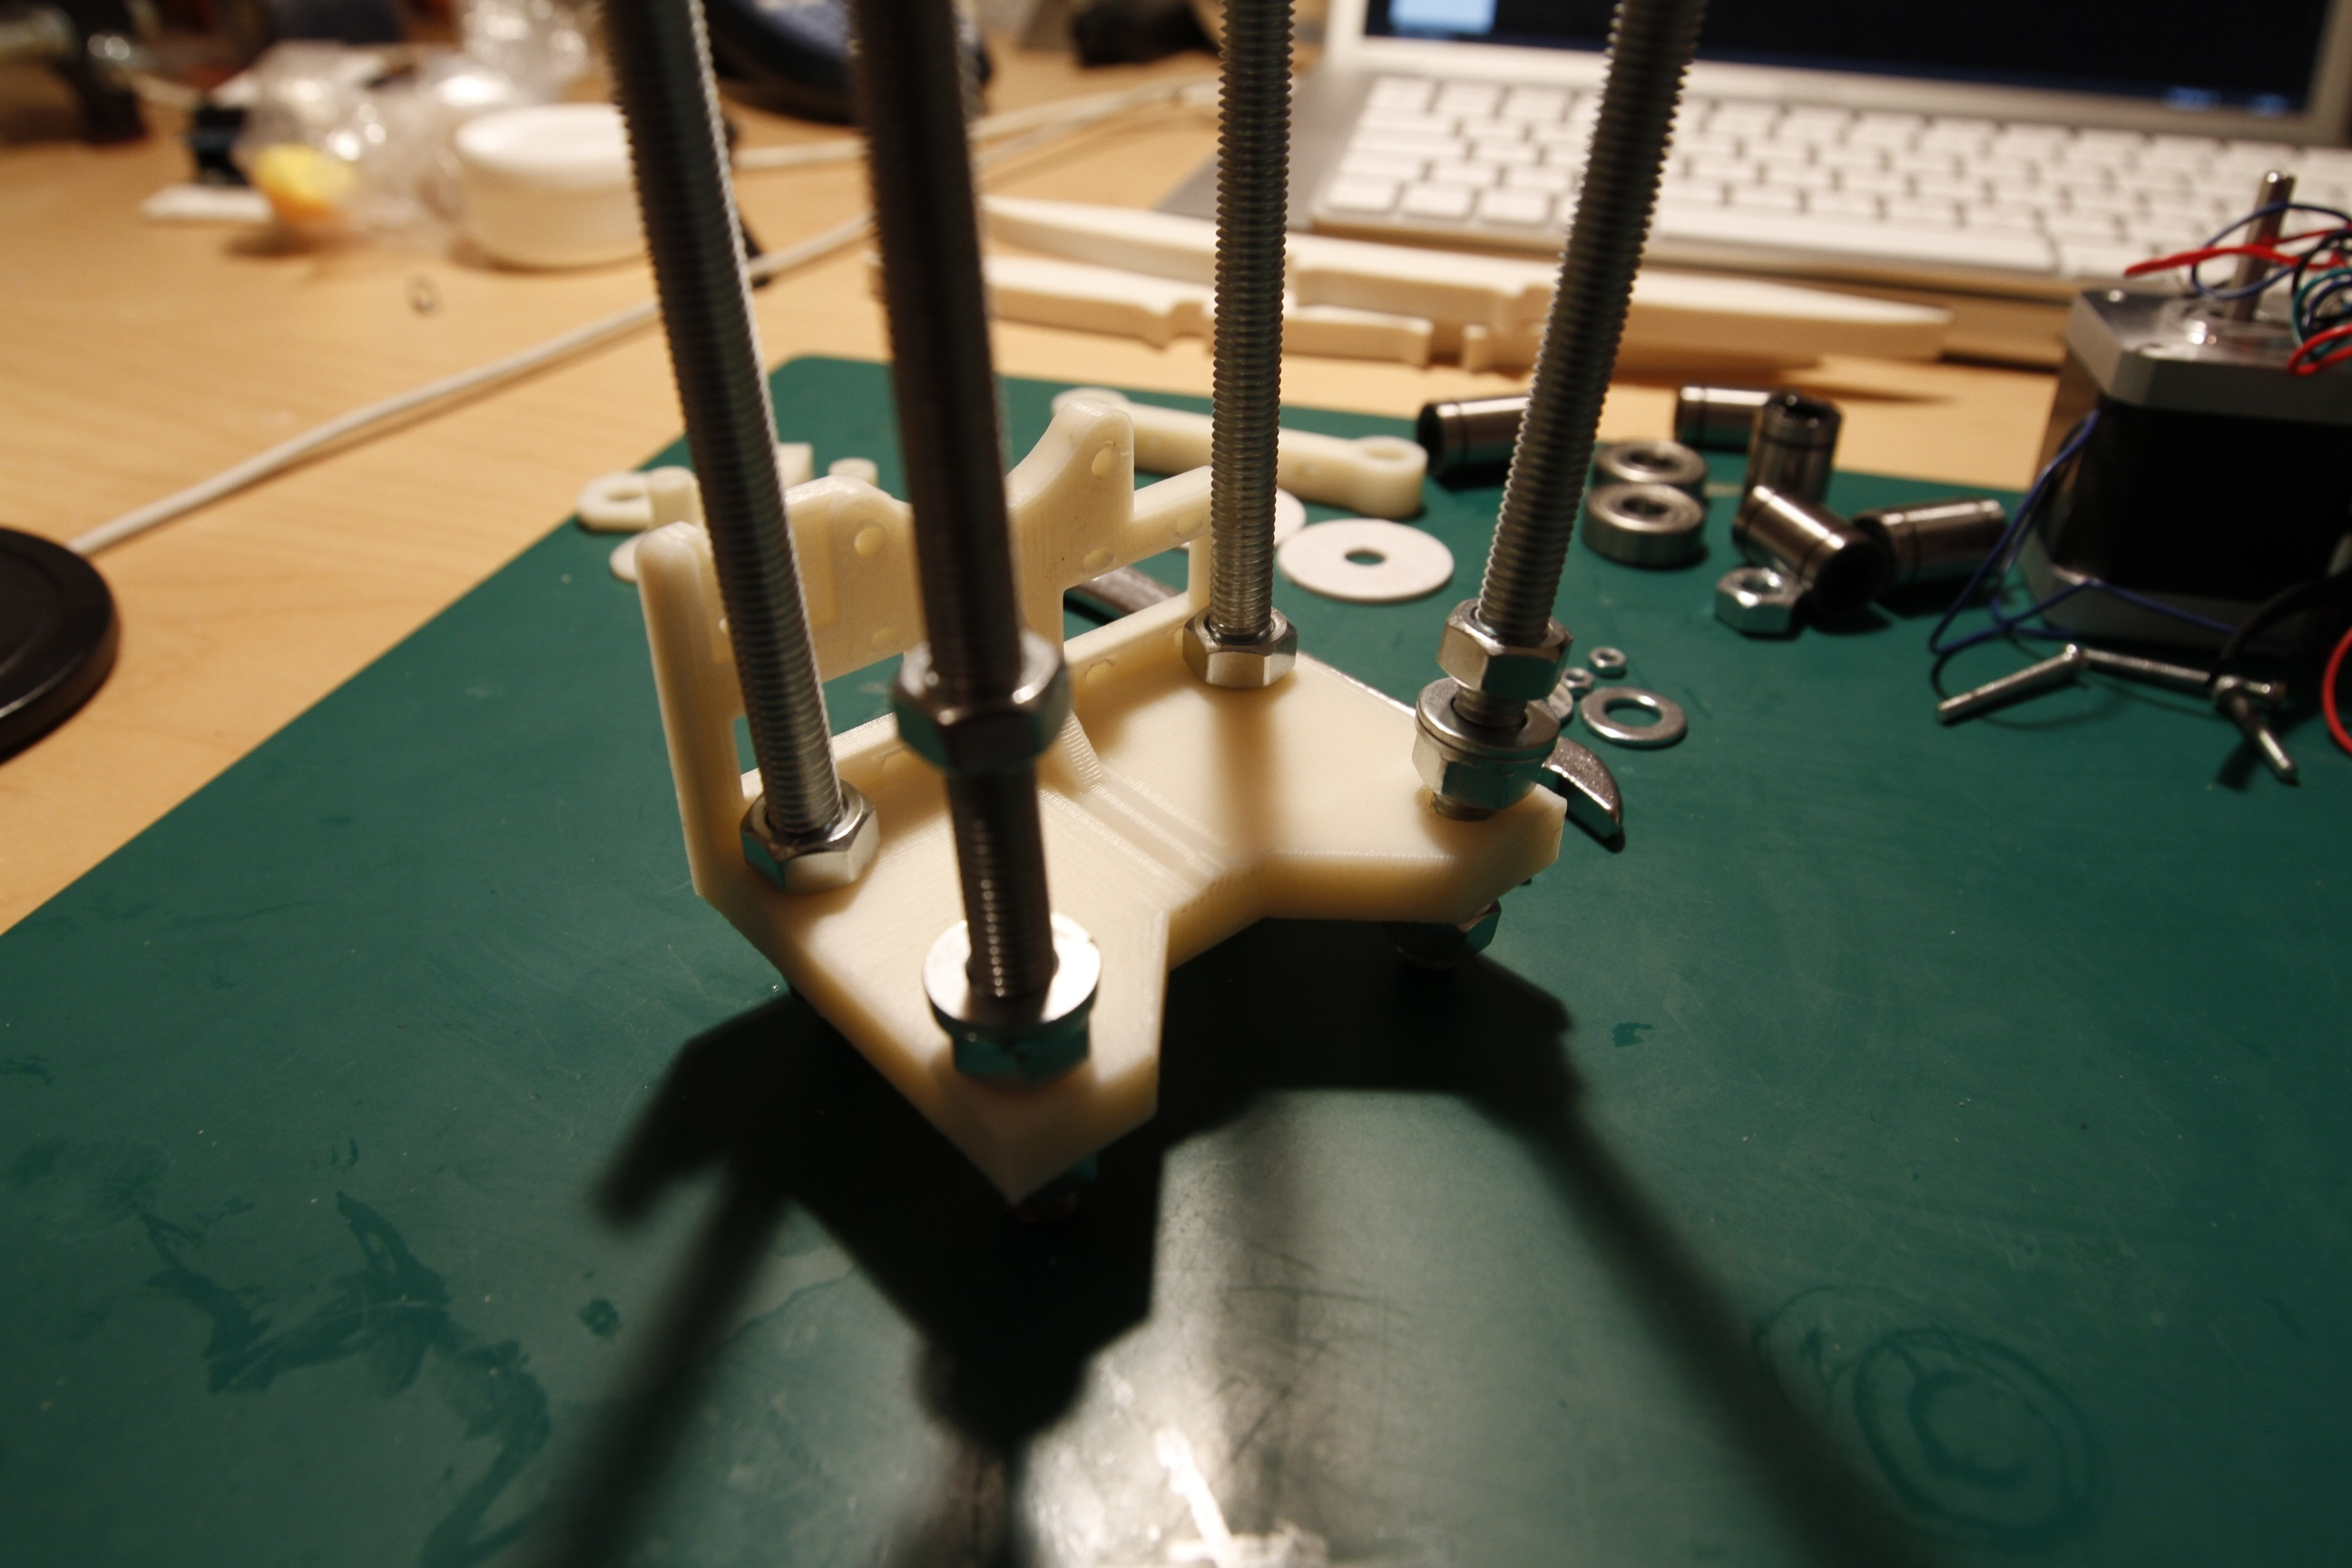
\includegraphics[width=0.6\textwidth]{../../Fotos/69.jpg}
			\caption{Lado izquierdo base}
			\label{fig:1.z}
		\end{figure}
		\begin{figure}[!htp]
			\centering
			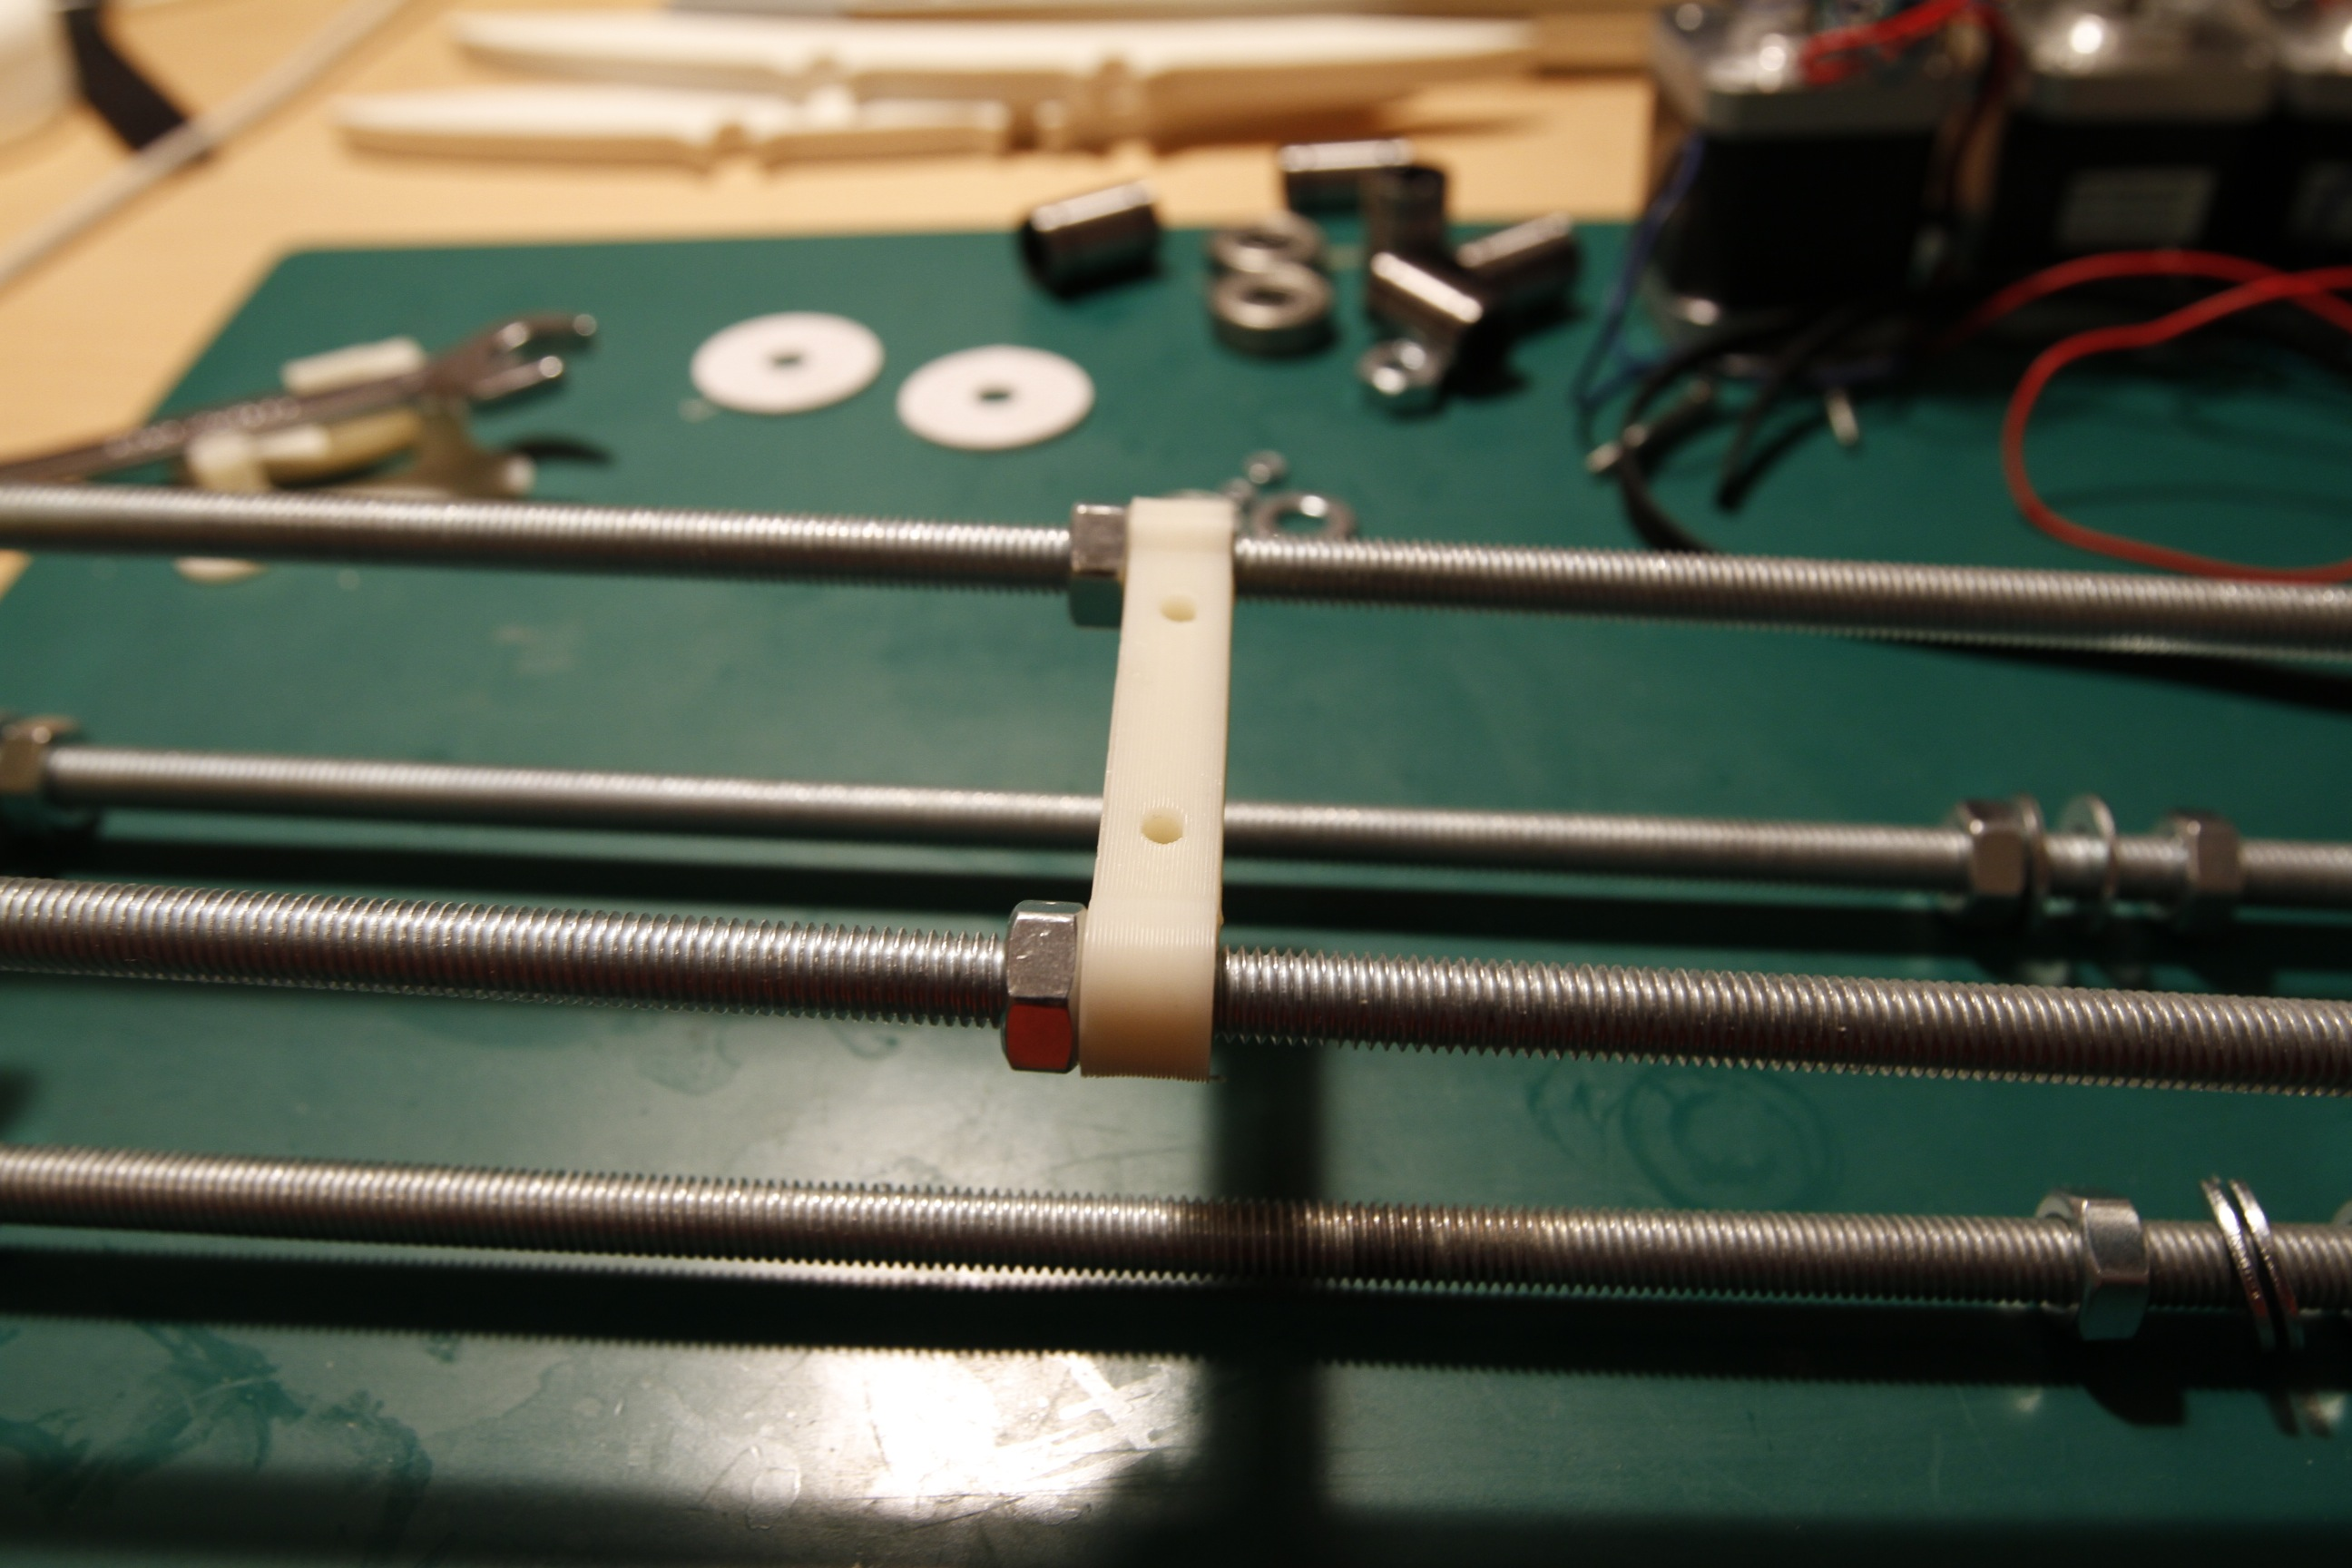
\includegraphics[width=0.6\textwidth]{../../Fotos/70.jpg}
			\caption{Centro base eje z}
			\label{fig:2.z}
		\end{figure}
		\begin{figure}[!htp]
			\centering
			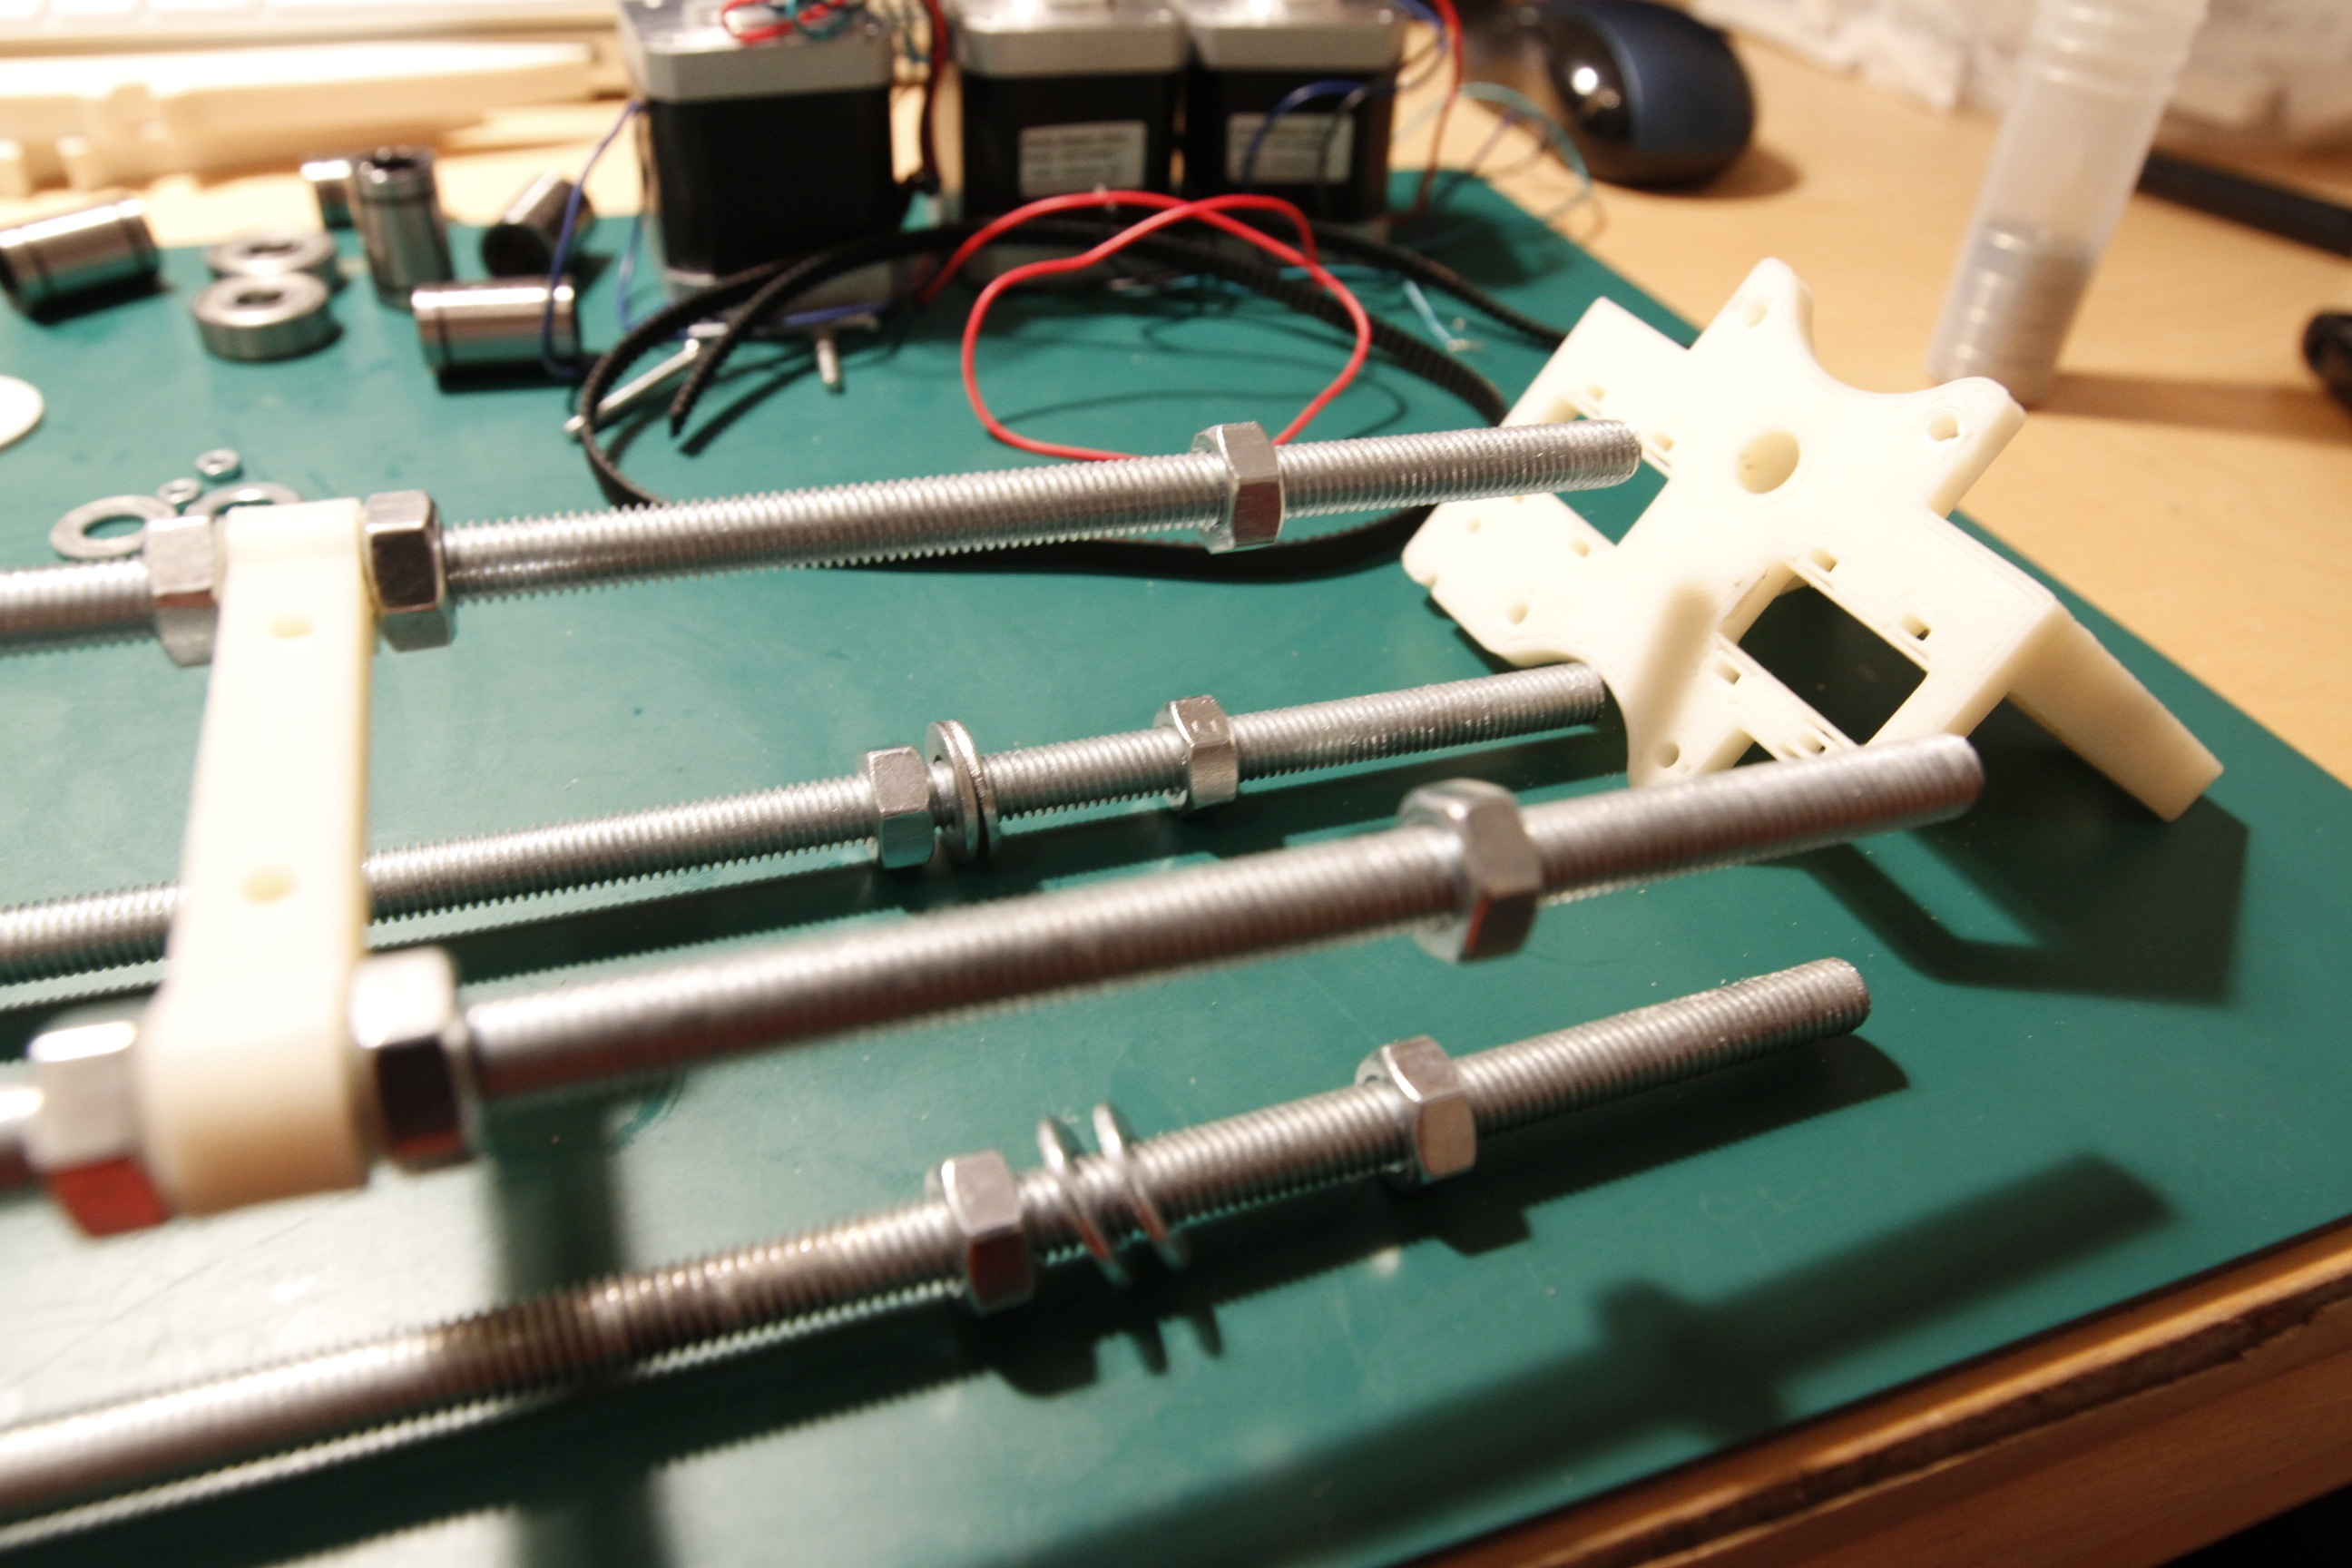
\includegraphics[width=0.6\textwidth]{../../Fotos/72.jpg}
			\caption{Lado derecho base}
			\label{fig:3.z}
		\end{figure}
		Es muy importante colocar la pieza para el endstop en la parte izquierda del eje Z, esta pieza determinará el lado izquierdo y derecho del eje Z durante todo el manual.
		\begin{figure}[!htp]
			\centering
			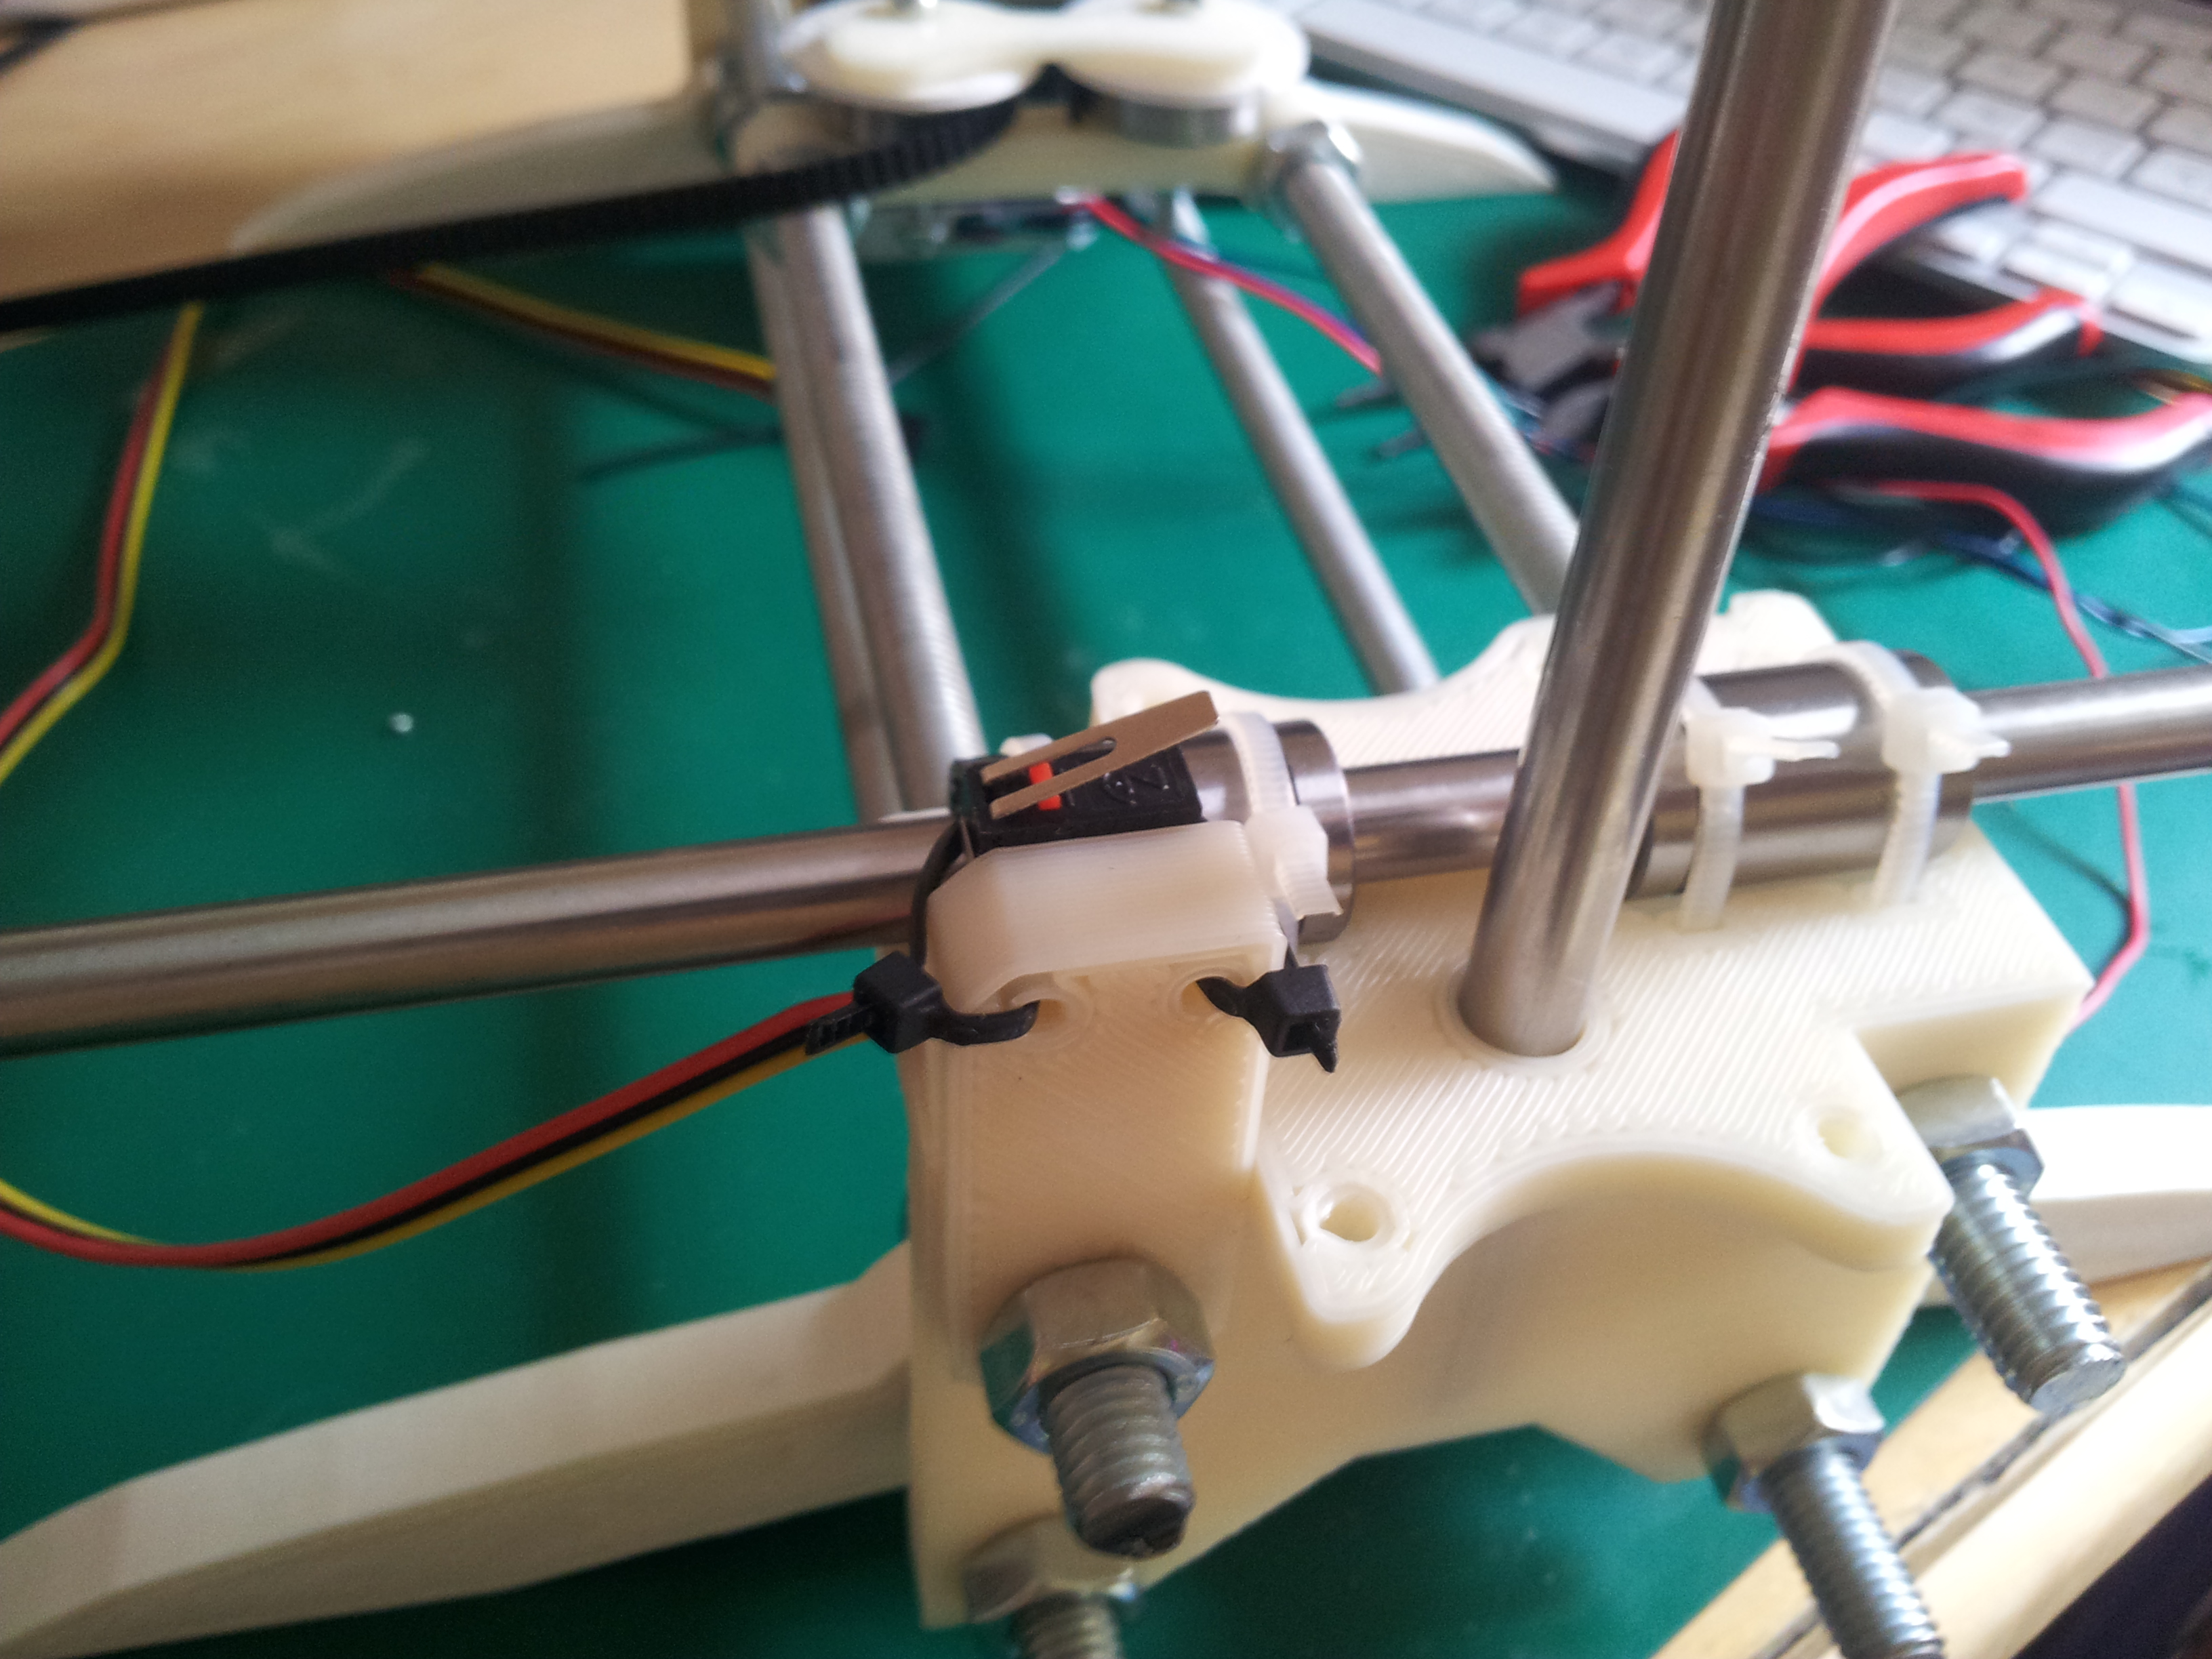
\includegraphics[width=0.6\textwidth]{../../Fotos/78.jpg}
			\caption{Soporte End-stop eje Z}
			\label{fig:4.z}
		\end{figure}
		Una vez colocadas las dos piezas de la base, el soporte del end-stop y las tuercas, apretaremos todas las tuercas del lado izquierdo. Lo siguiente será colocar los cuatro rodamientos lineales para colocar la base del eje Y, ya que está determinará la distancia del eje Z. Ver imagen ~\ref{fig:7.z}. Todavía no es necesario apretar del todo las bridas, eso se hará más adelante.
		\begin{figure}[H]
		        \centering
		        \begin{subfigure}[htb]{0.5\textwidth}
		                \centering
		                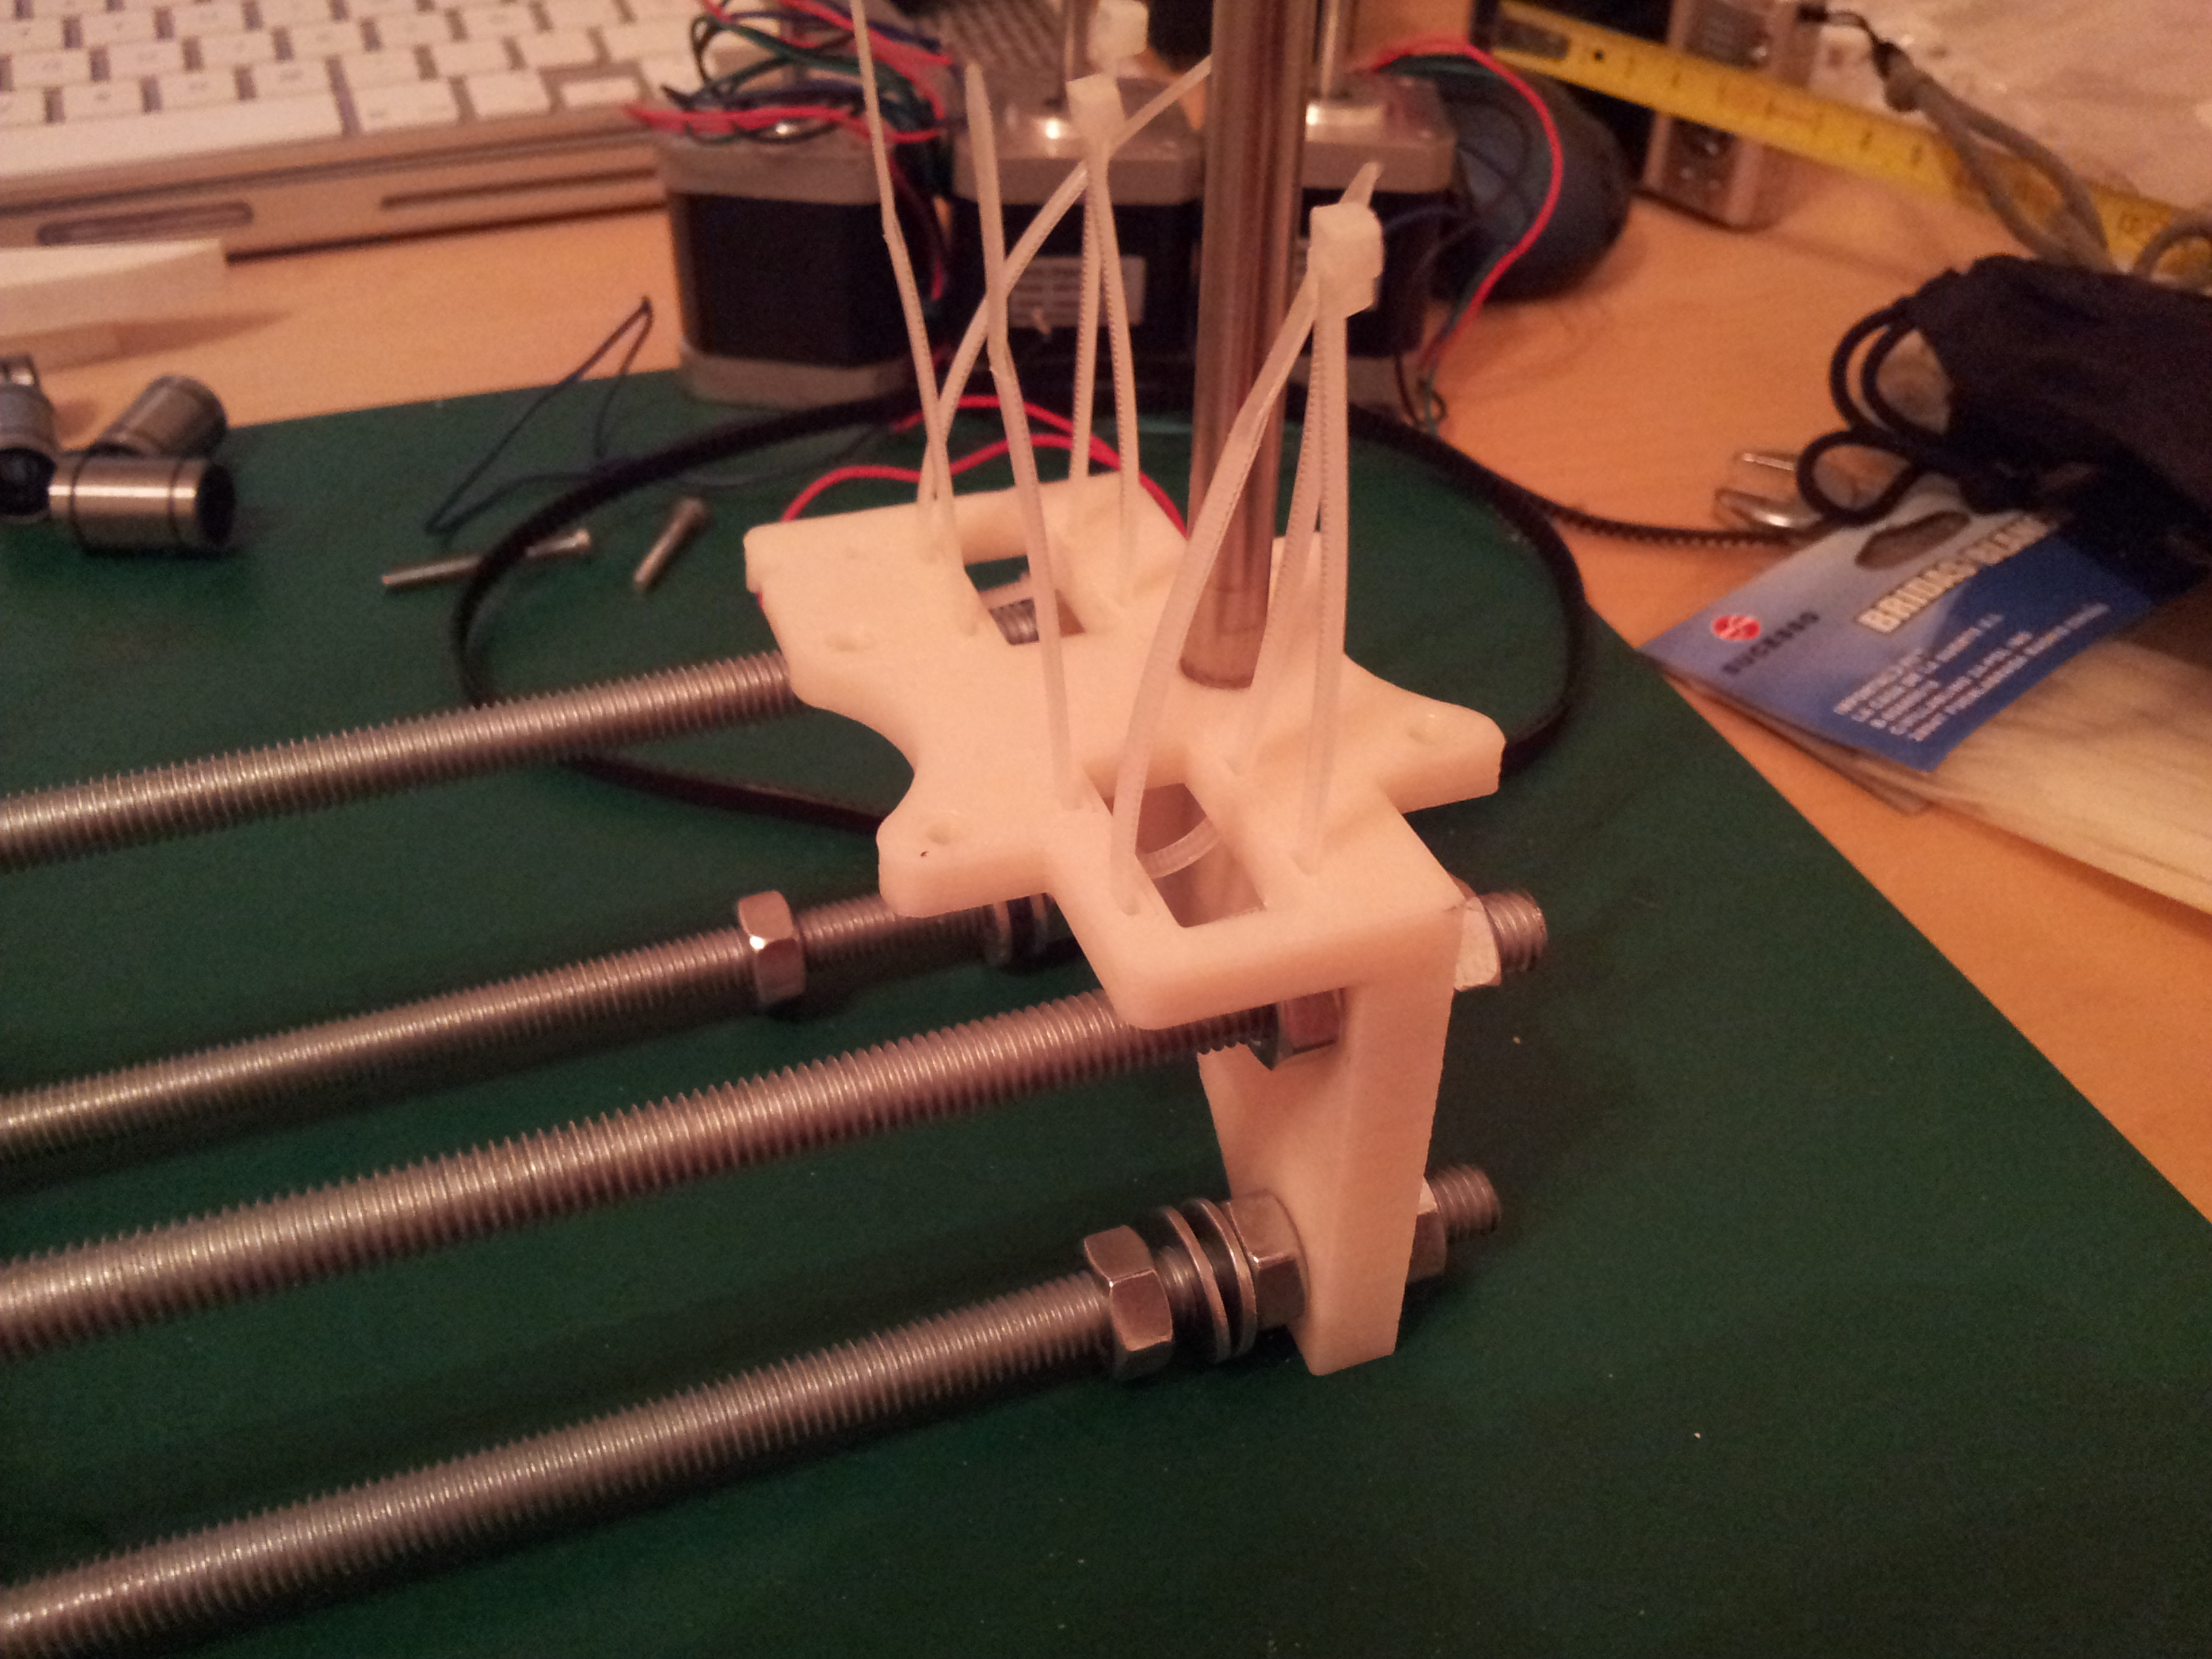
\includegraphics[width=\textwidth]{../../Fotos/76.jpg}
		                \caption{Bridas para rodamientos lineales}
		                \label{fig:5.z}
		        \end{subfigure}
		        \begin{subfigure}[htb]{0.5\textwidth}
		                \centering
		                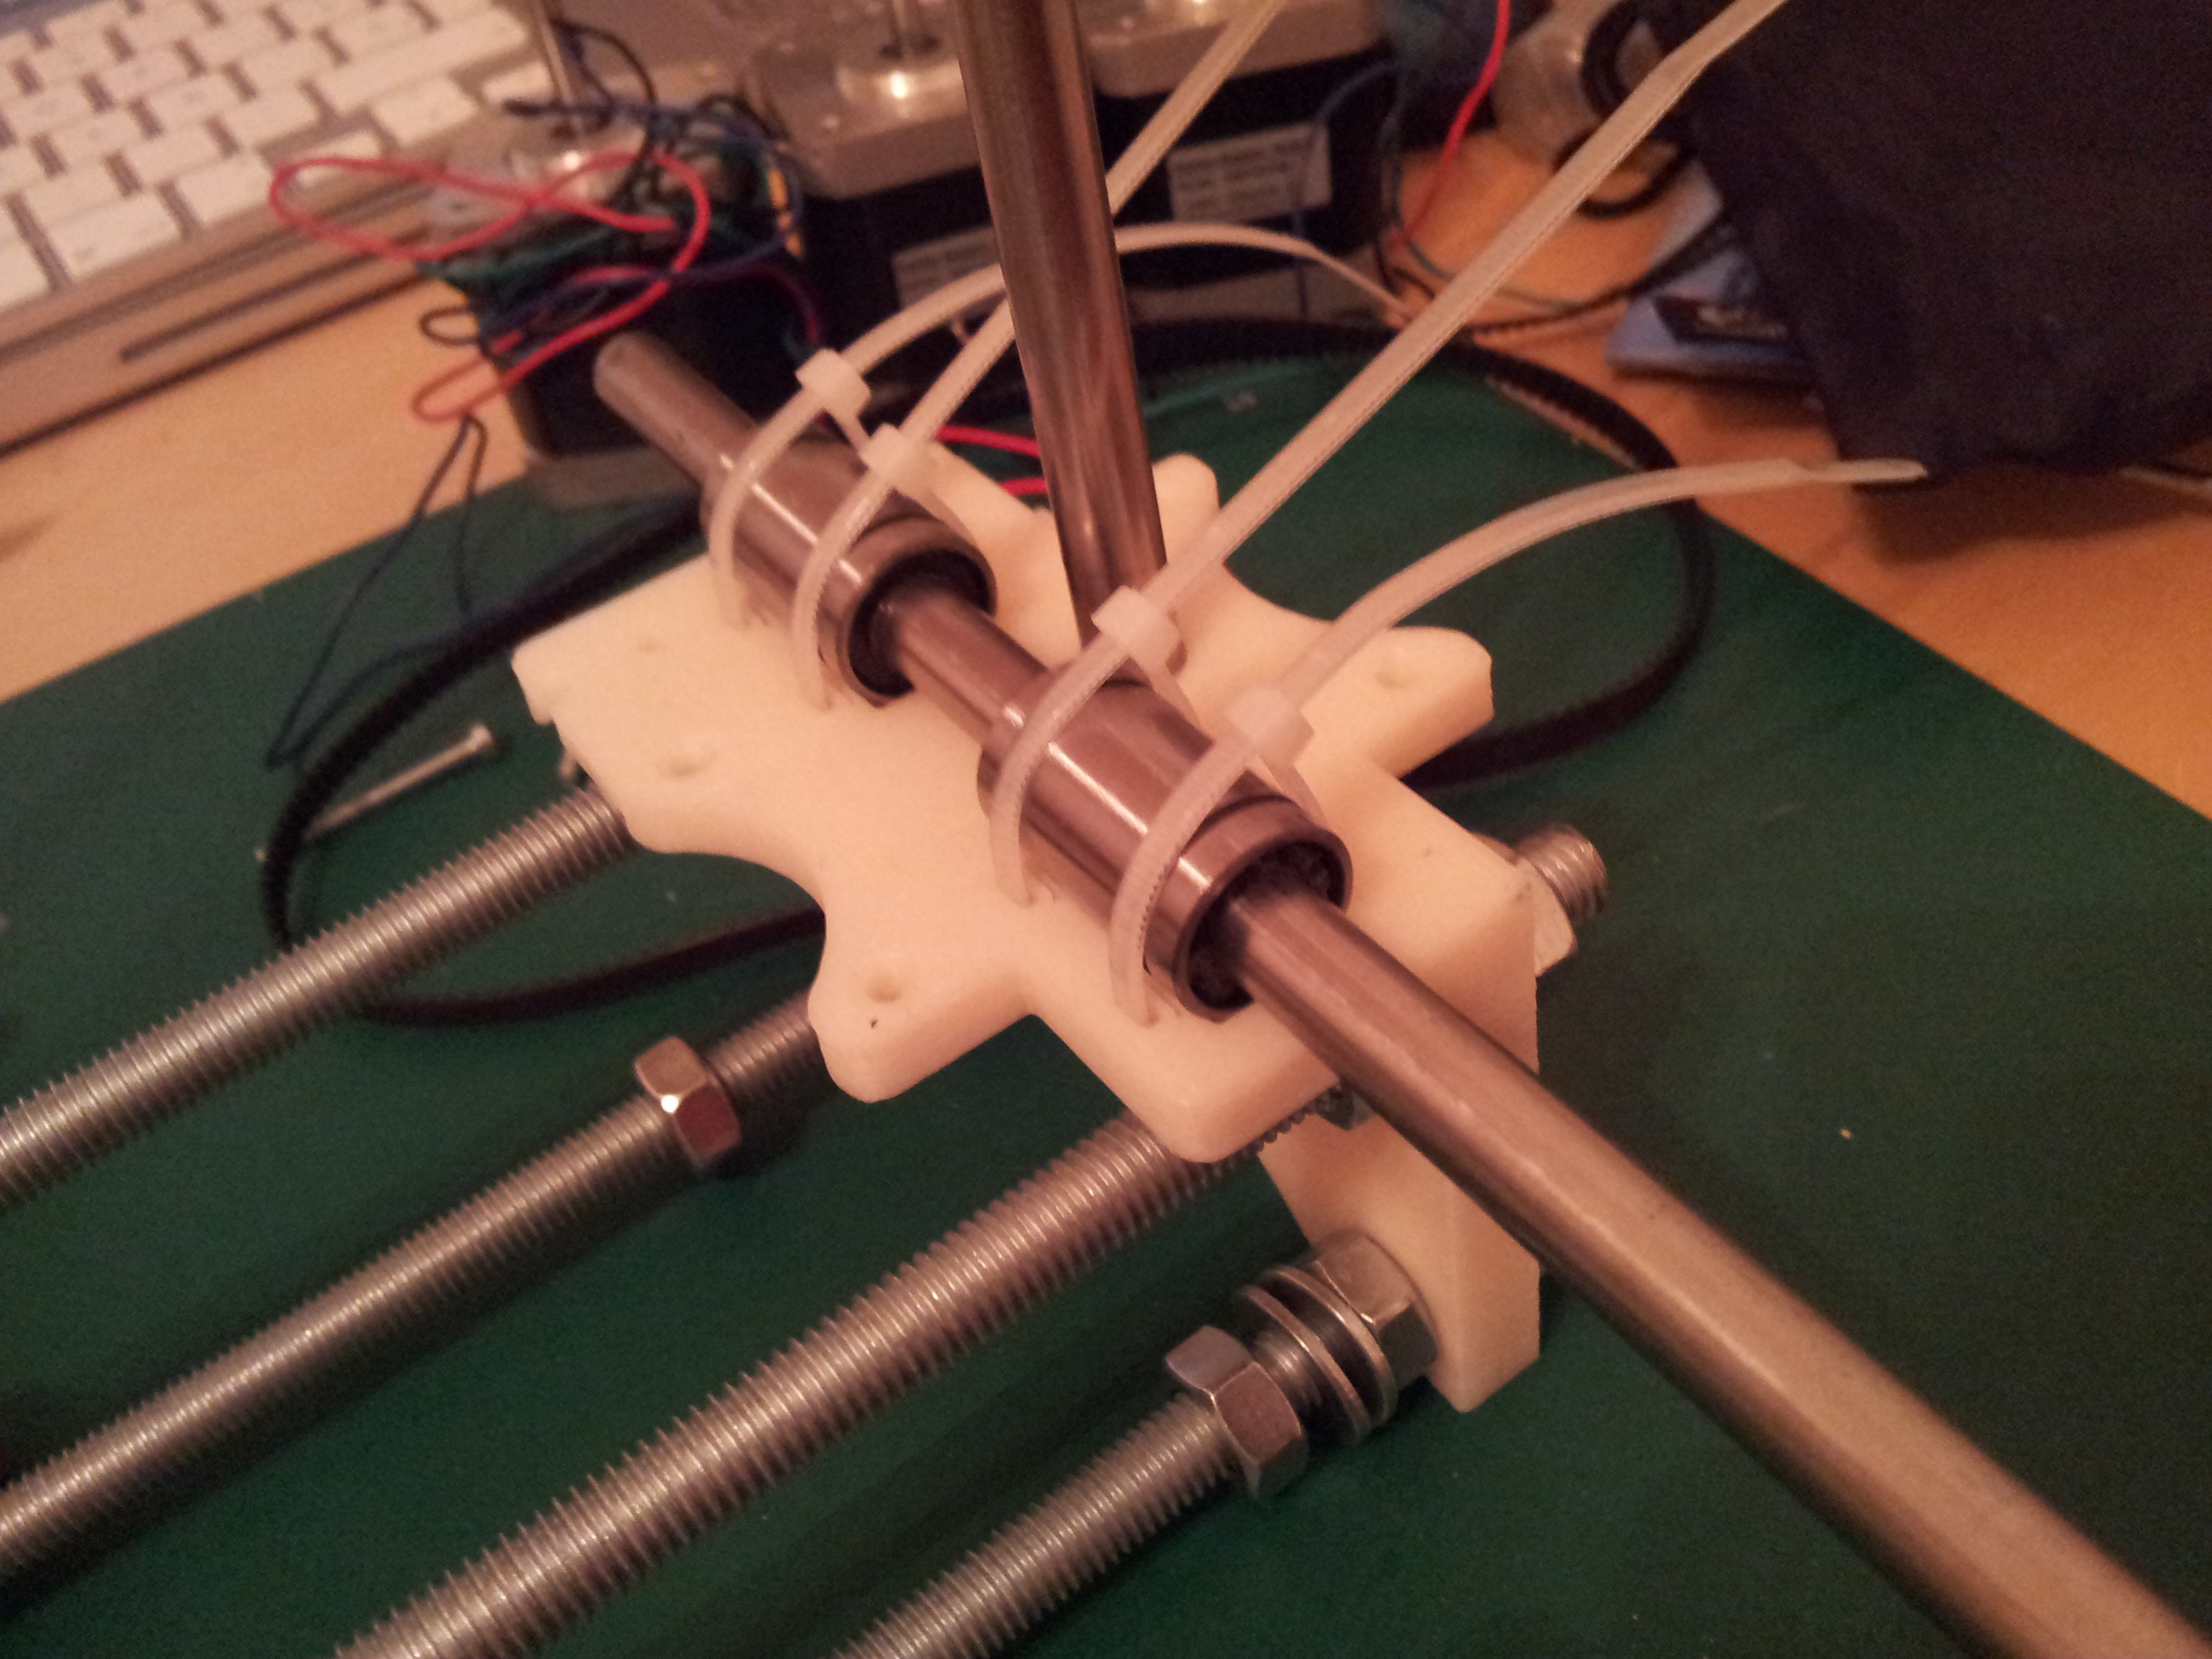
\includegraphics[width=\textwidth]{../../Fotos/77.jpg}
		                \caption{Rodamientos lineales colocados}
		                \label{fig:6.z}
		        \end{subfigure}
		        \caption{Colocando los rodamientos lineales del eje Z}\label{fig:7.z}
		\end{figure}
		Una vez colocados los rodamientos lineales, presentamos el eje Y poniendolo en su posición y comprobamos que desliza correctamente. En este momento colocamos las varillas lisas del eje Z y medimos la distancia que hay entre la parte inferior y la superior. ( Ver imagen ~\ref{fig:10.z})
		\begin{figure}[H]
		        \centering
		        \begin{subfigure}[htb]{0.5\textwidth}
		                \centering
		                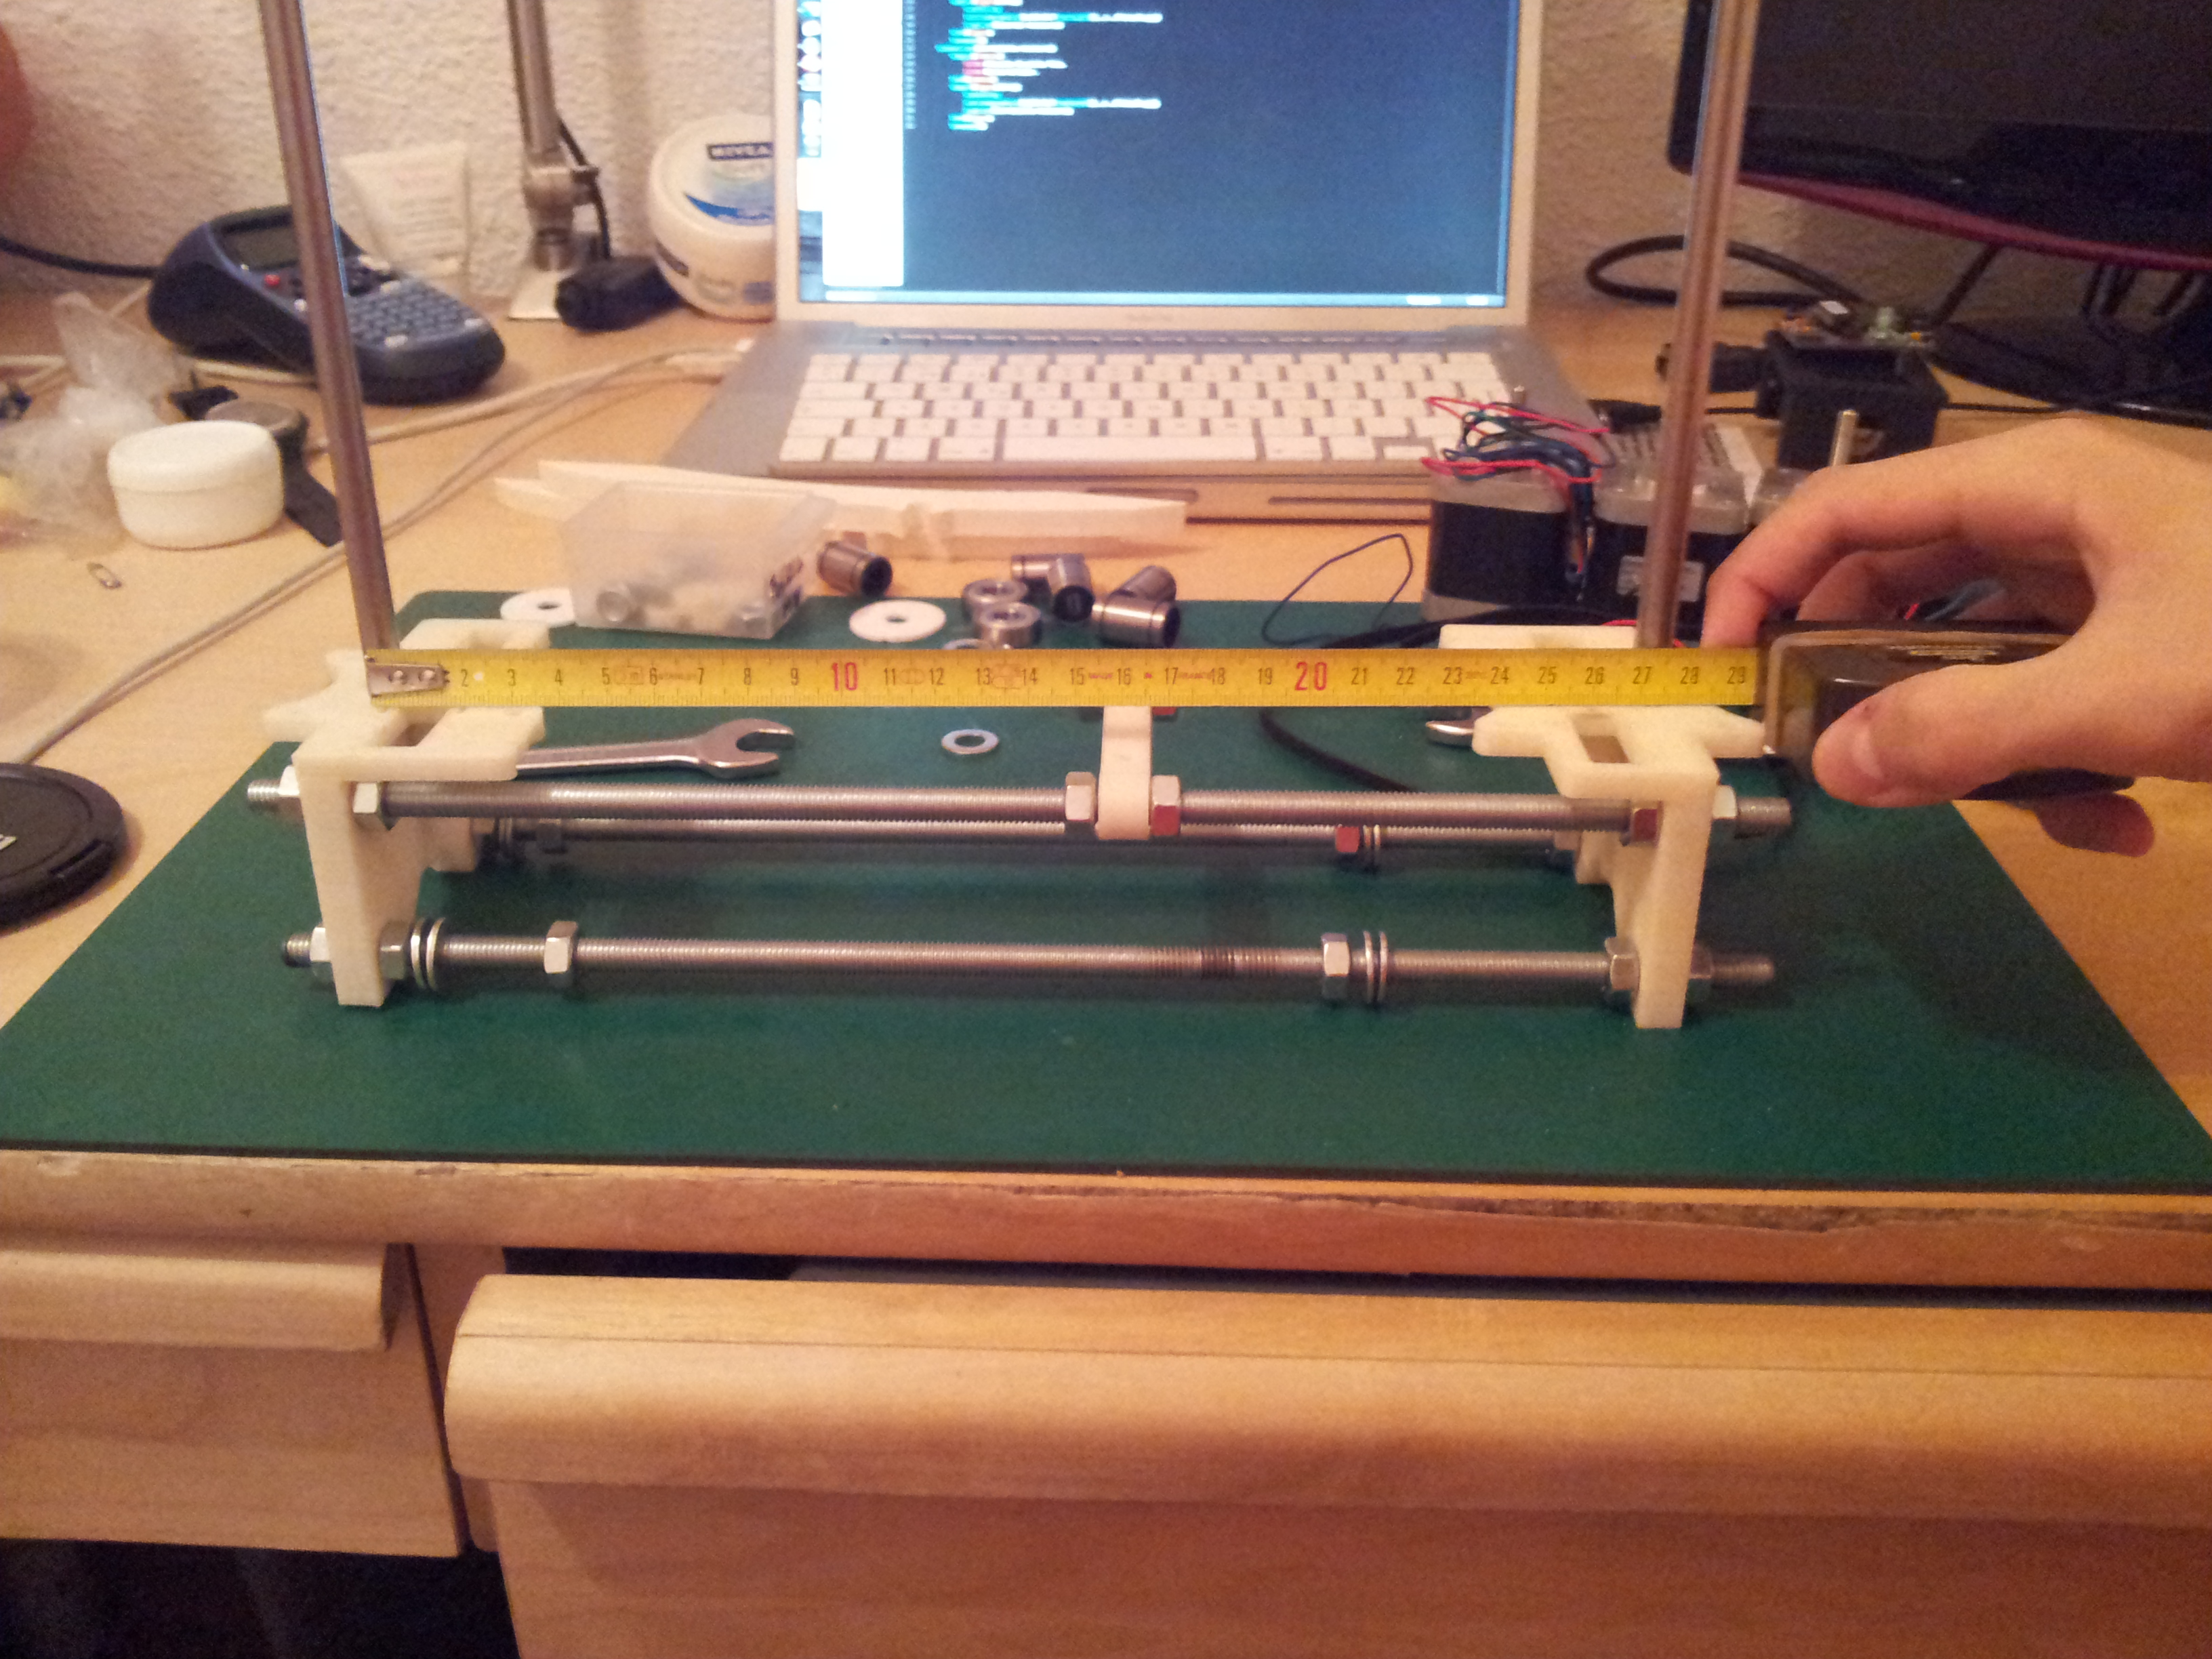
\includegraphics[width=\textwidth]{../../Fotos/74.jpg}
		                \caption{Distancia inferior varillas lisas}
		                \label{fig:8.z}
		        \end{subfigure}
		        \begin{subfigure}[htb]{0.5\textwidth}
		                \centering
		                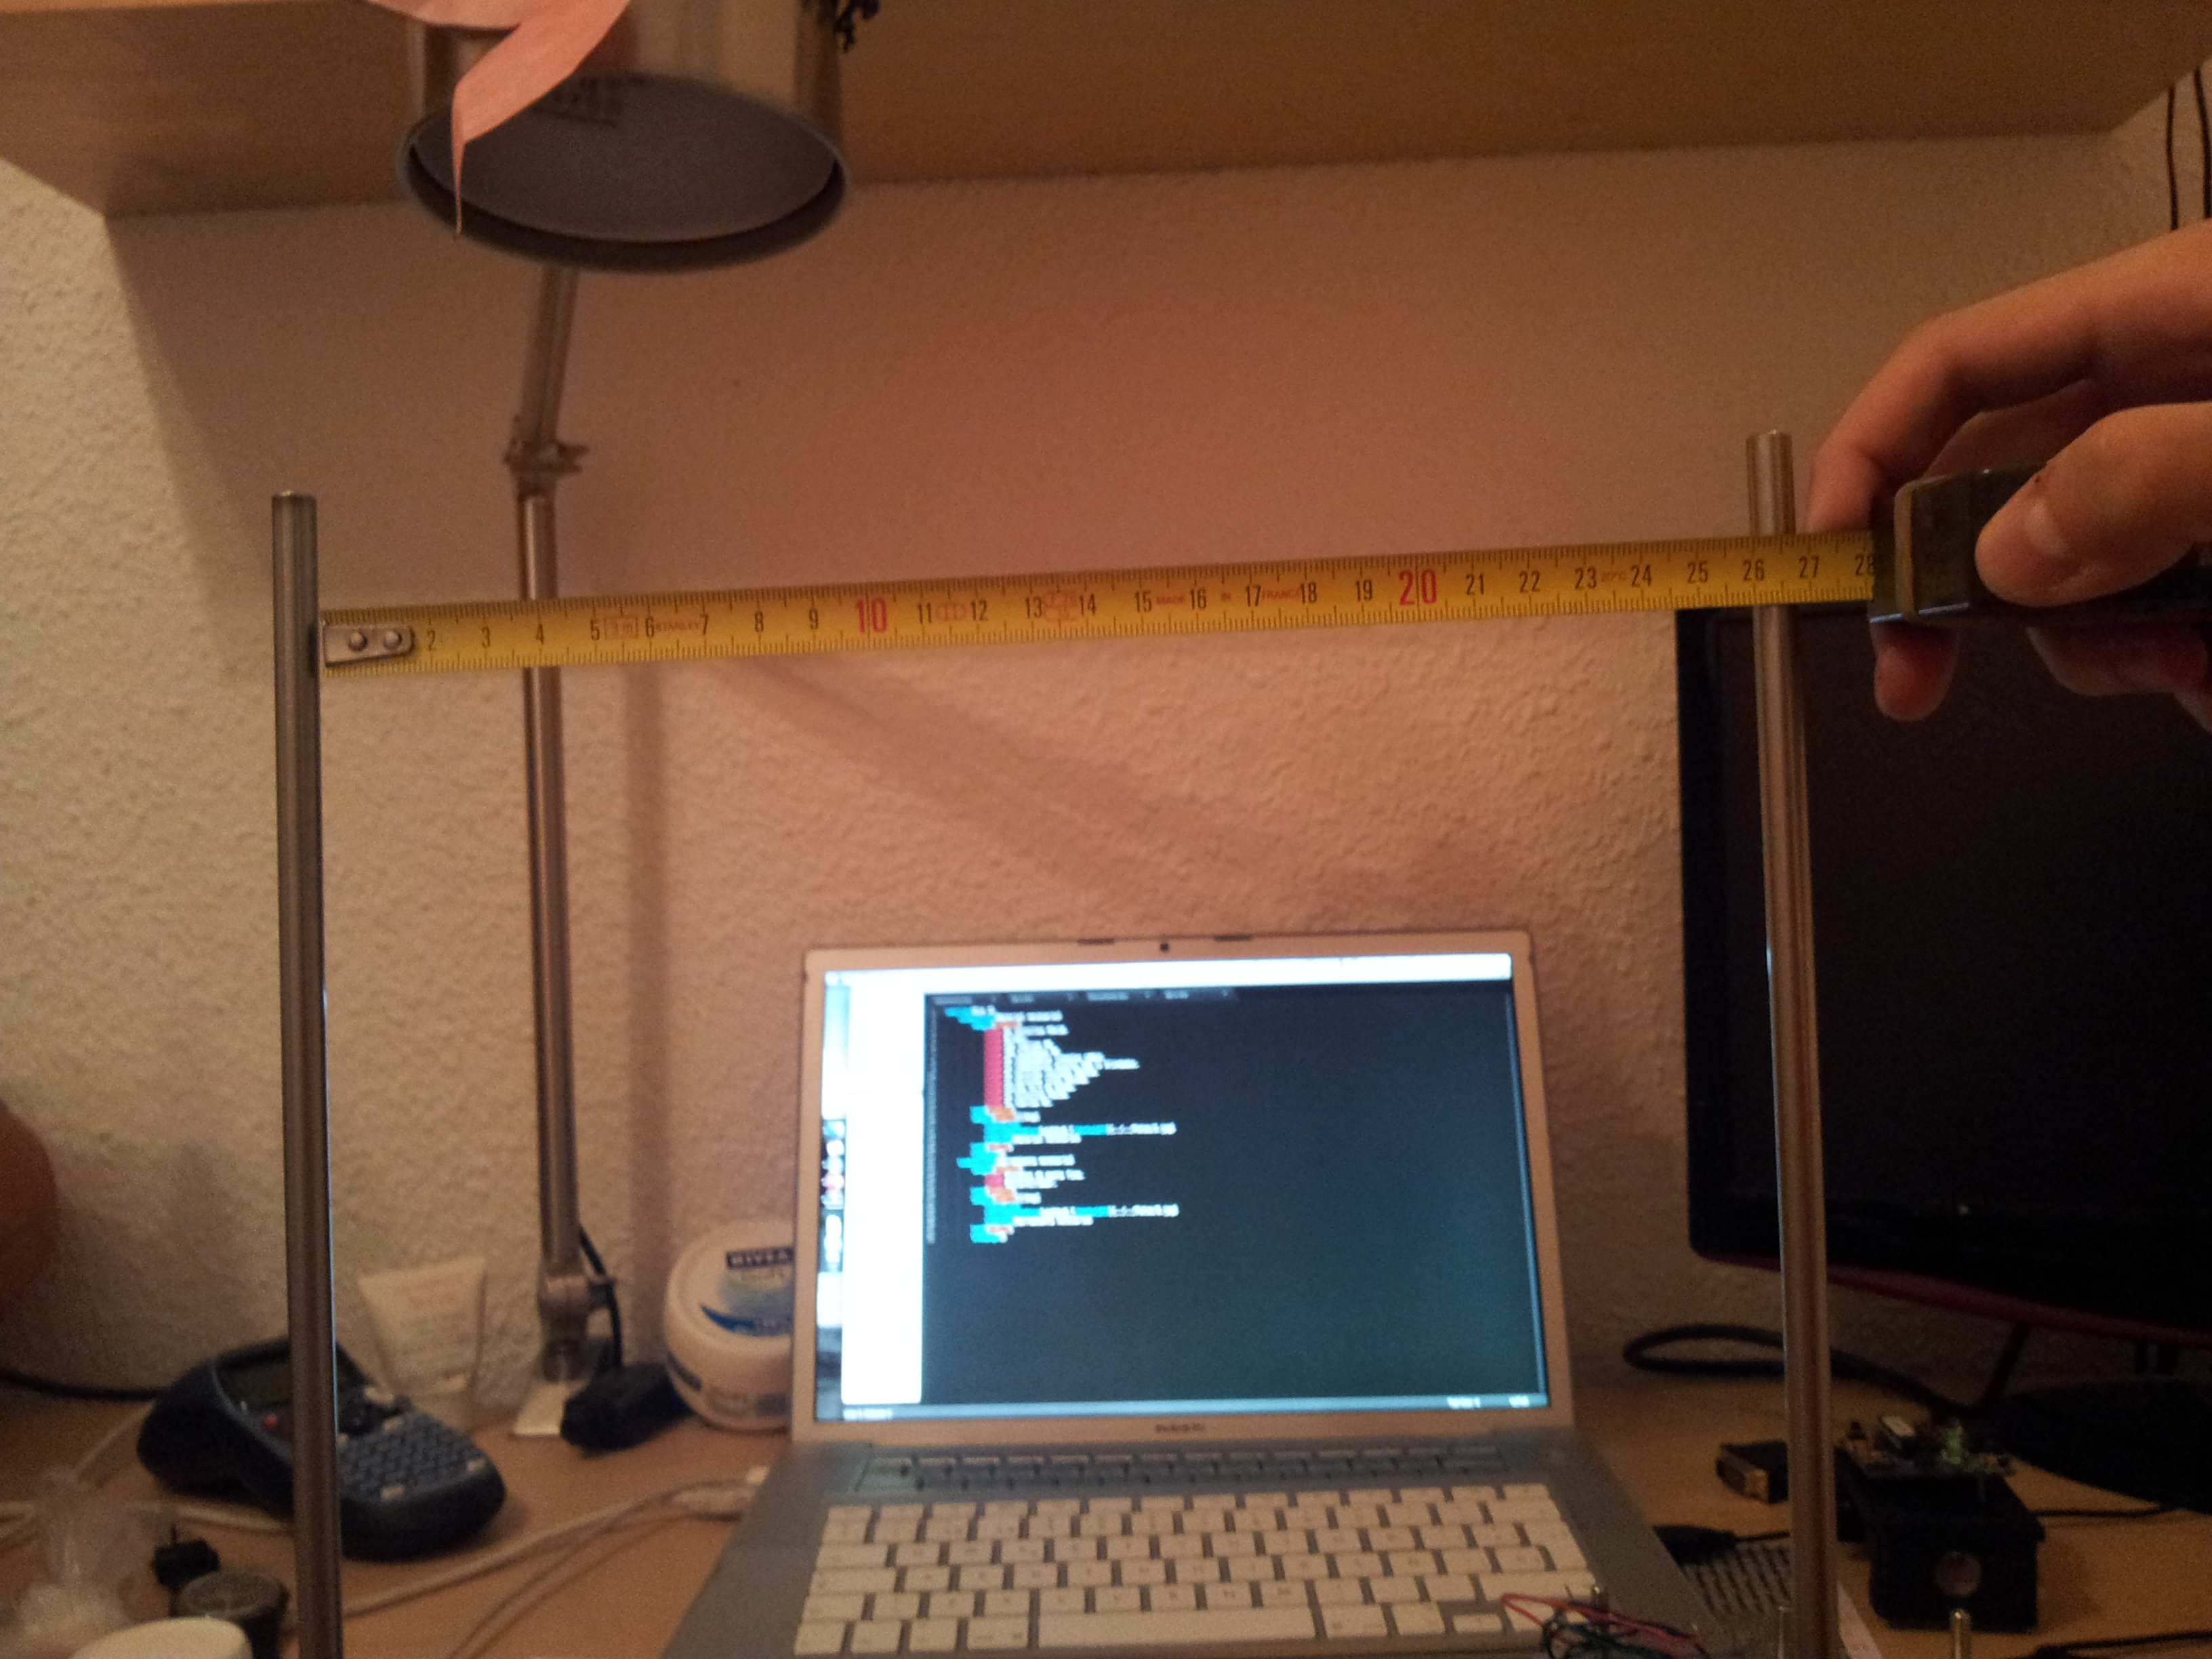
\includegraphics[width=\textwidth]{../../Fotos/75.jpg}
		                \caption{Distancia superior varillas lisas}
		                \label{fig:9.z}
		        \end{subfigure}
		        \caption{Colocando los rodamientos lineales del eje Z}\label{fig:10.z}
		\end{figure}
		Para hacer que en la parte superior y en la inferior haya la misma distancia, iremos apretando o aflojando las tuercas del lado derecho de la base. Este paso es muy importante ya que determinará el correcto funcionamiento del eje Z. Por último, para comprobar que está bien nivelado, introduciremos el eje X por los rodamientos lineales y comprobaremos que somos capaces de subir y bajar toda la estructura. Si en algún tramo notamos algún rozamiento, comprobaremos otra vez la distancia en todos los tramos del eje Z.
		Para continuar, montaremos el conjunto encargado de guiar la correa dentada del eje Y.
		Para ello usaremos dos rodamientos axiales, las dos arandelas impresas, la pieza Y Bearing Guide y dos tornillos de M3x30. Lo montaremos como se muestra en la imagen ~\ref{fig:13.z}) y lo colocaremos en la pieza que se ve en la figura ~\ref{fig:2.z}
		\begin{figure}[H]
		        \centering
		        \begin{subfigure}[htb]{0.5\textwidth}
		                \centering
		                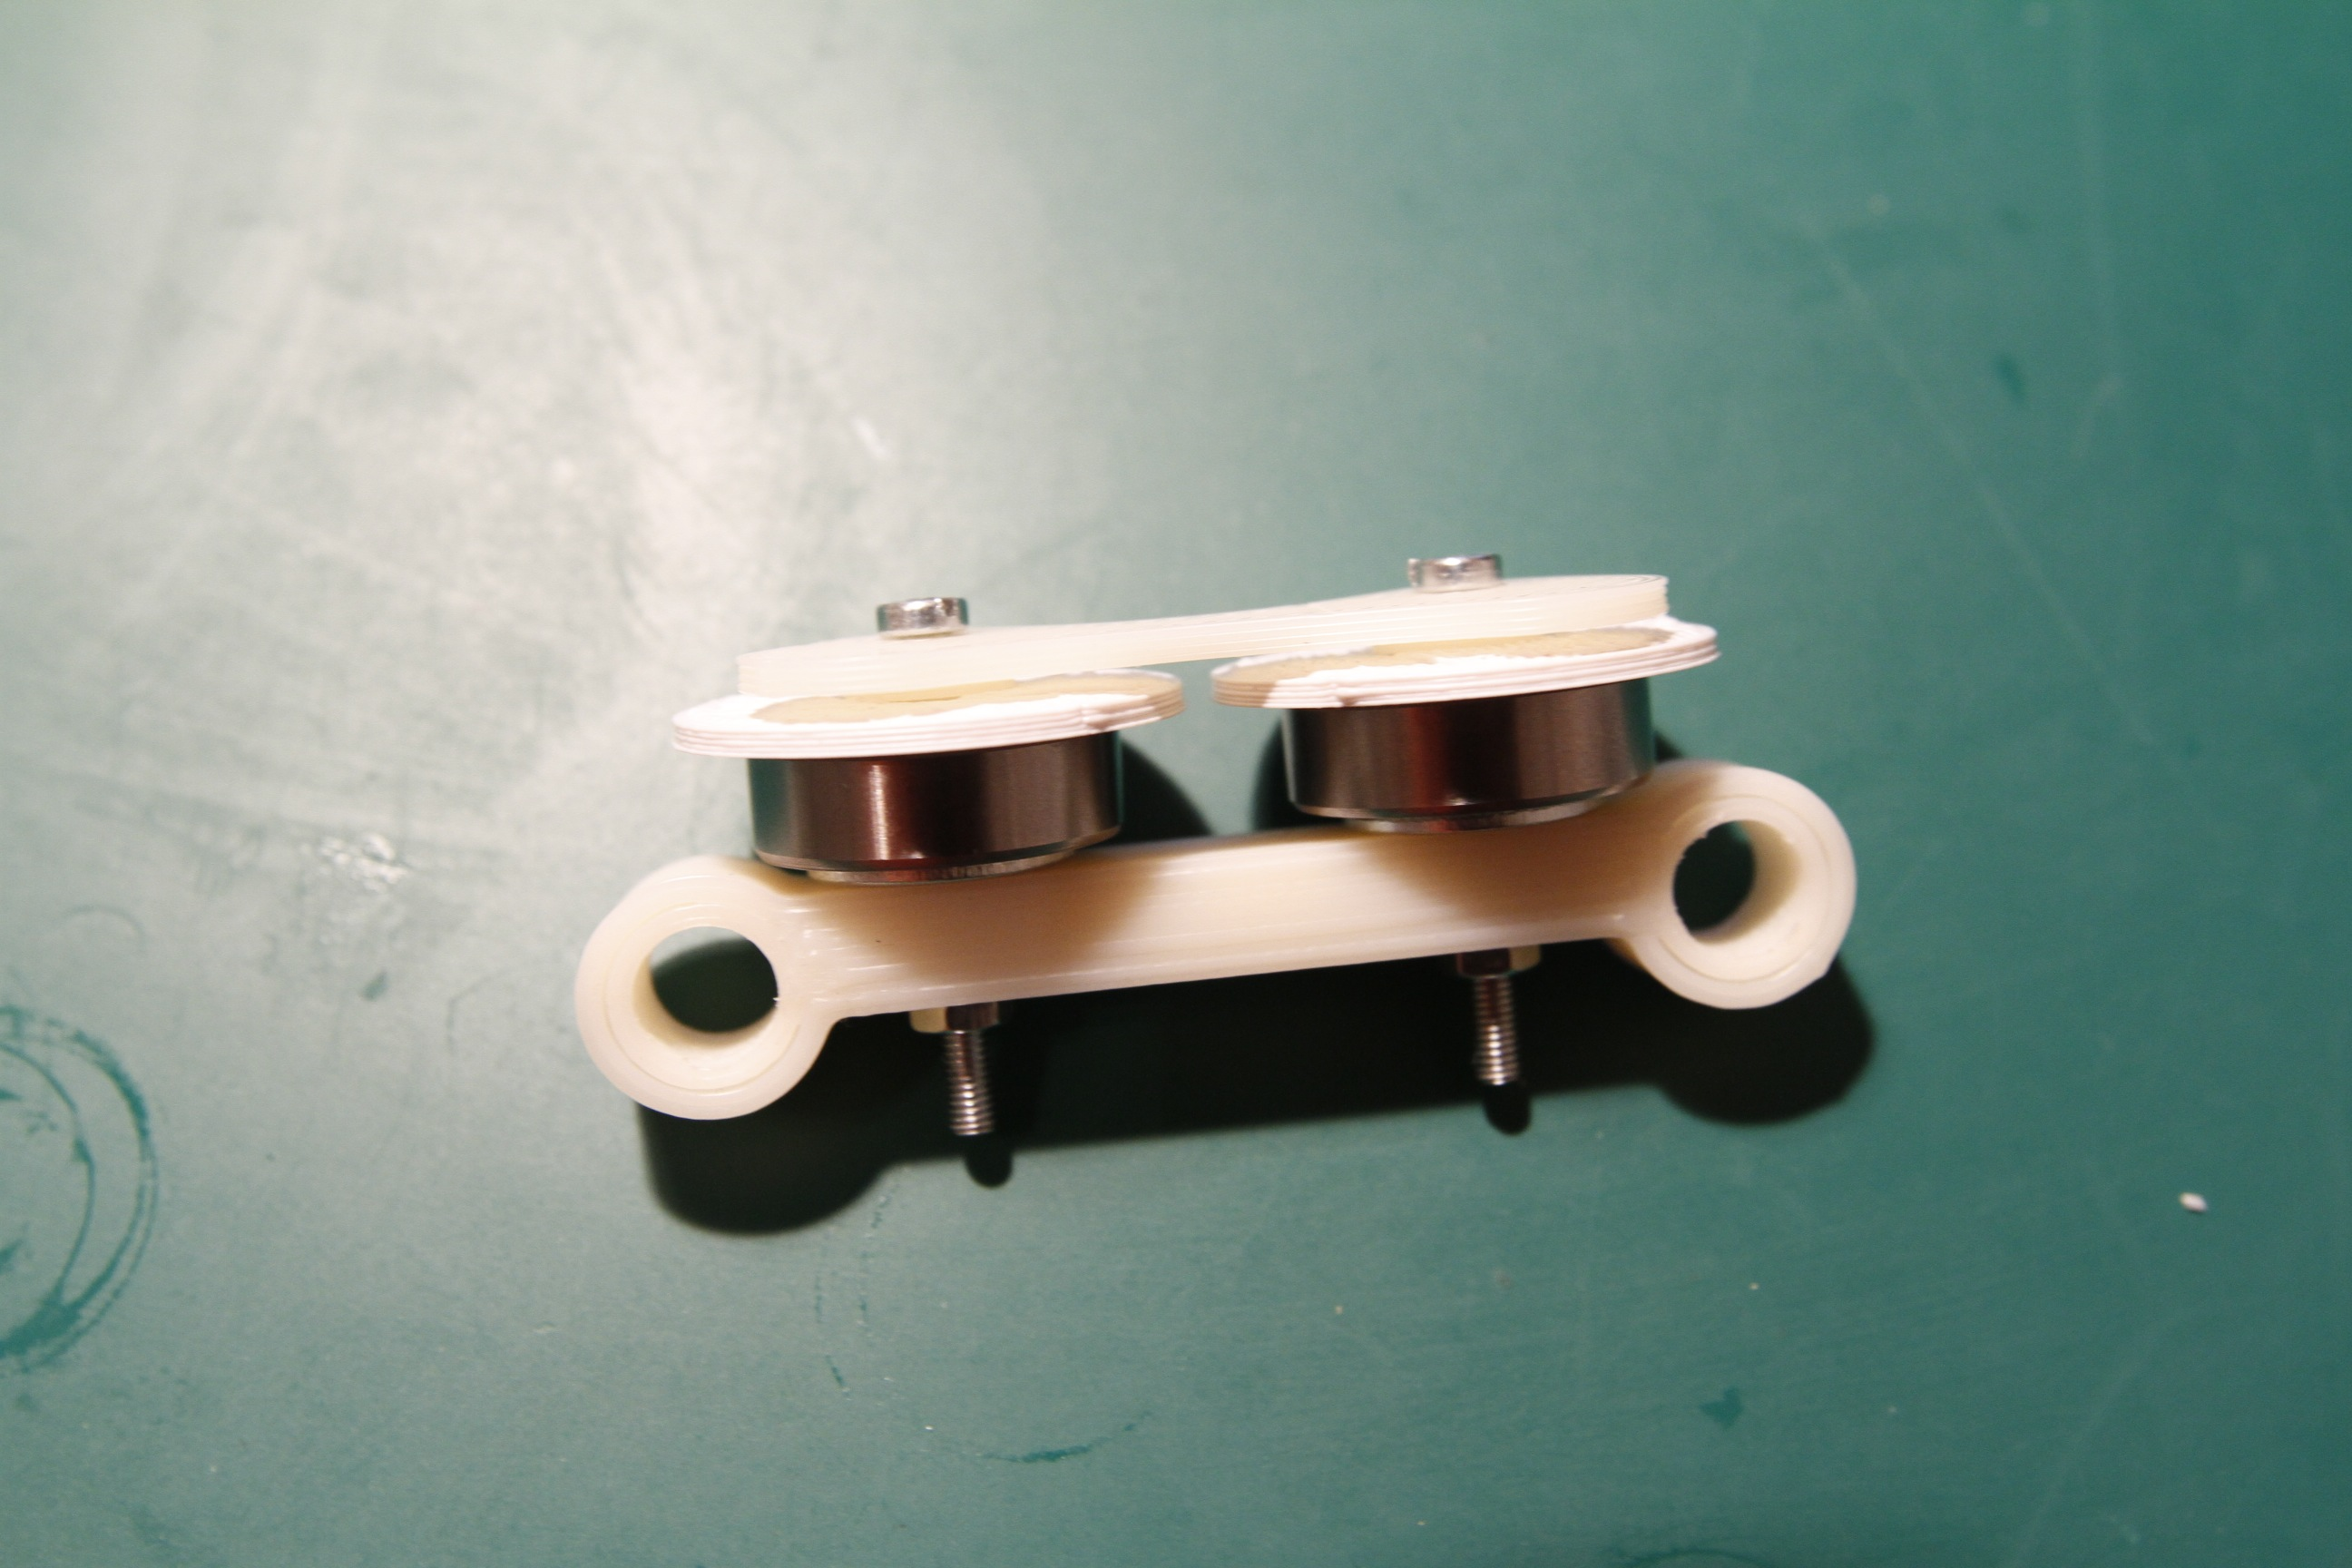
\includegraphics[width=\textwidth]{../../Fotos/71.jpg}
		                %\caption{Bearing Guide del eje Y}
		                \label{fig:11.z}
		        \end{subfigure}
		        \begin{subfigure}[htb]{0.5\textwidth}
		                \centering
		                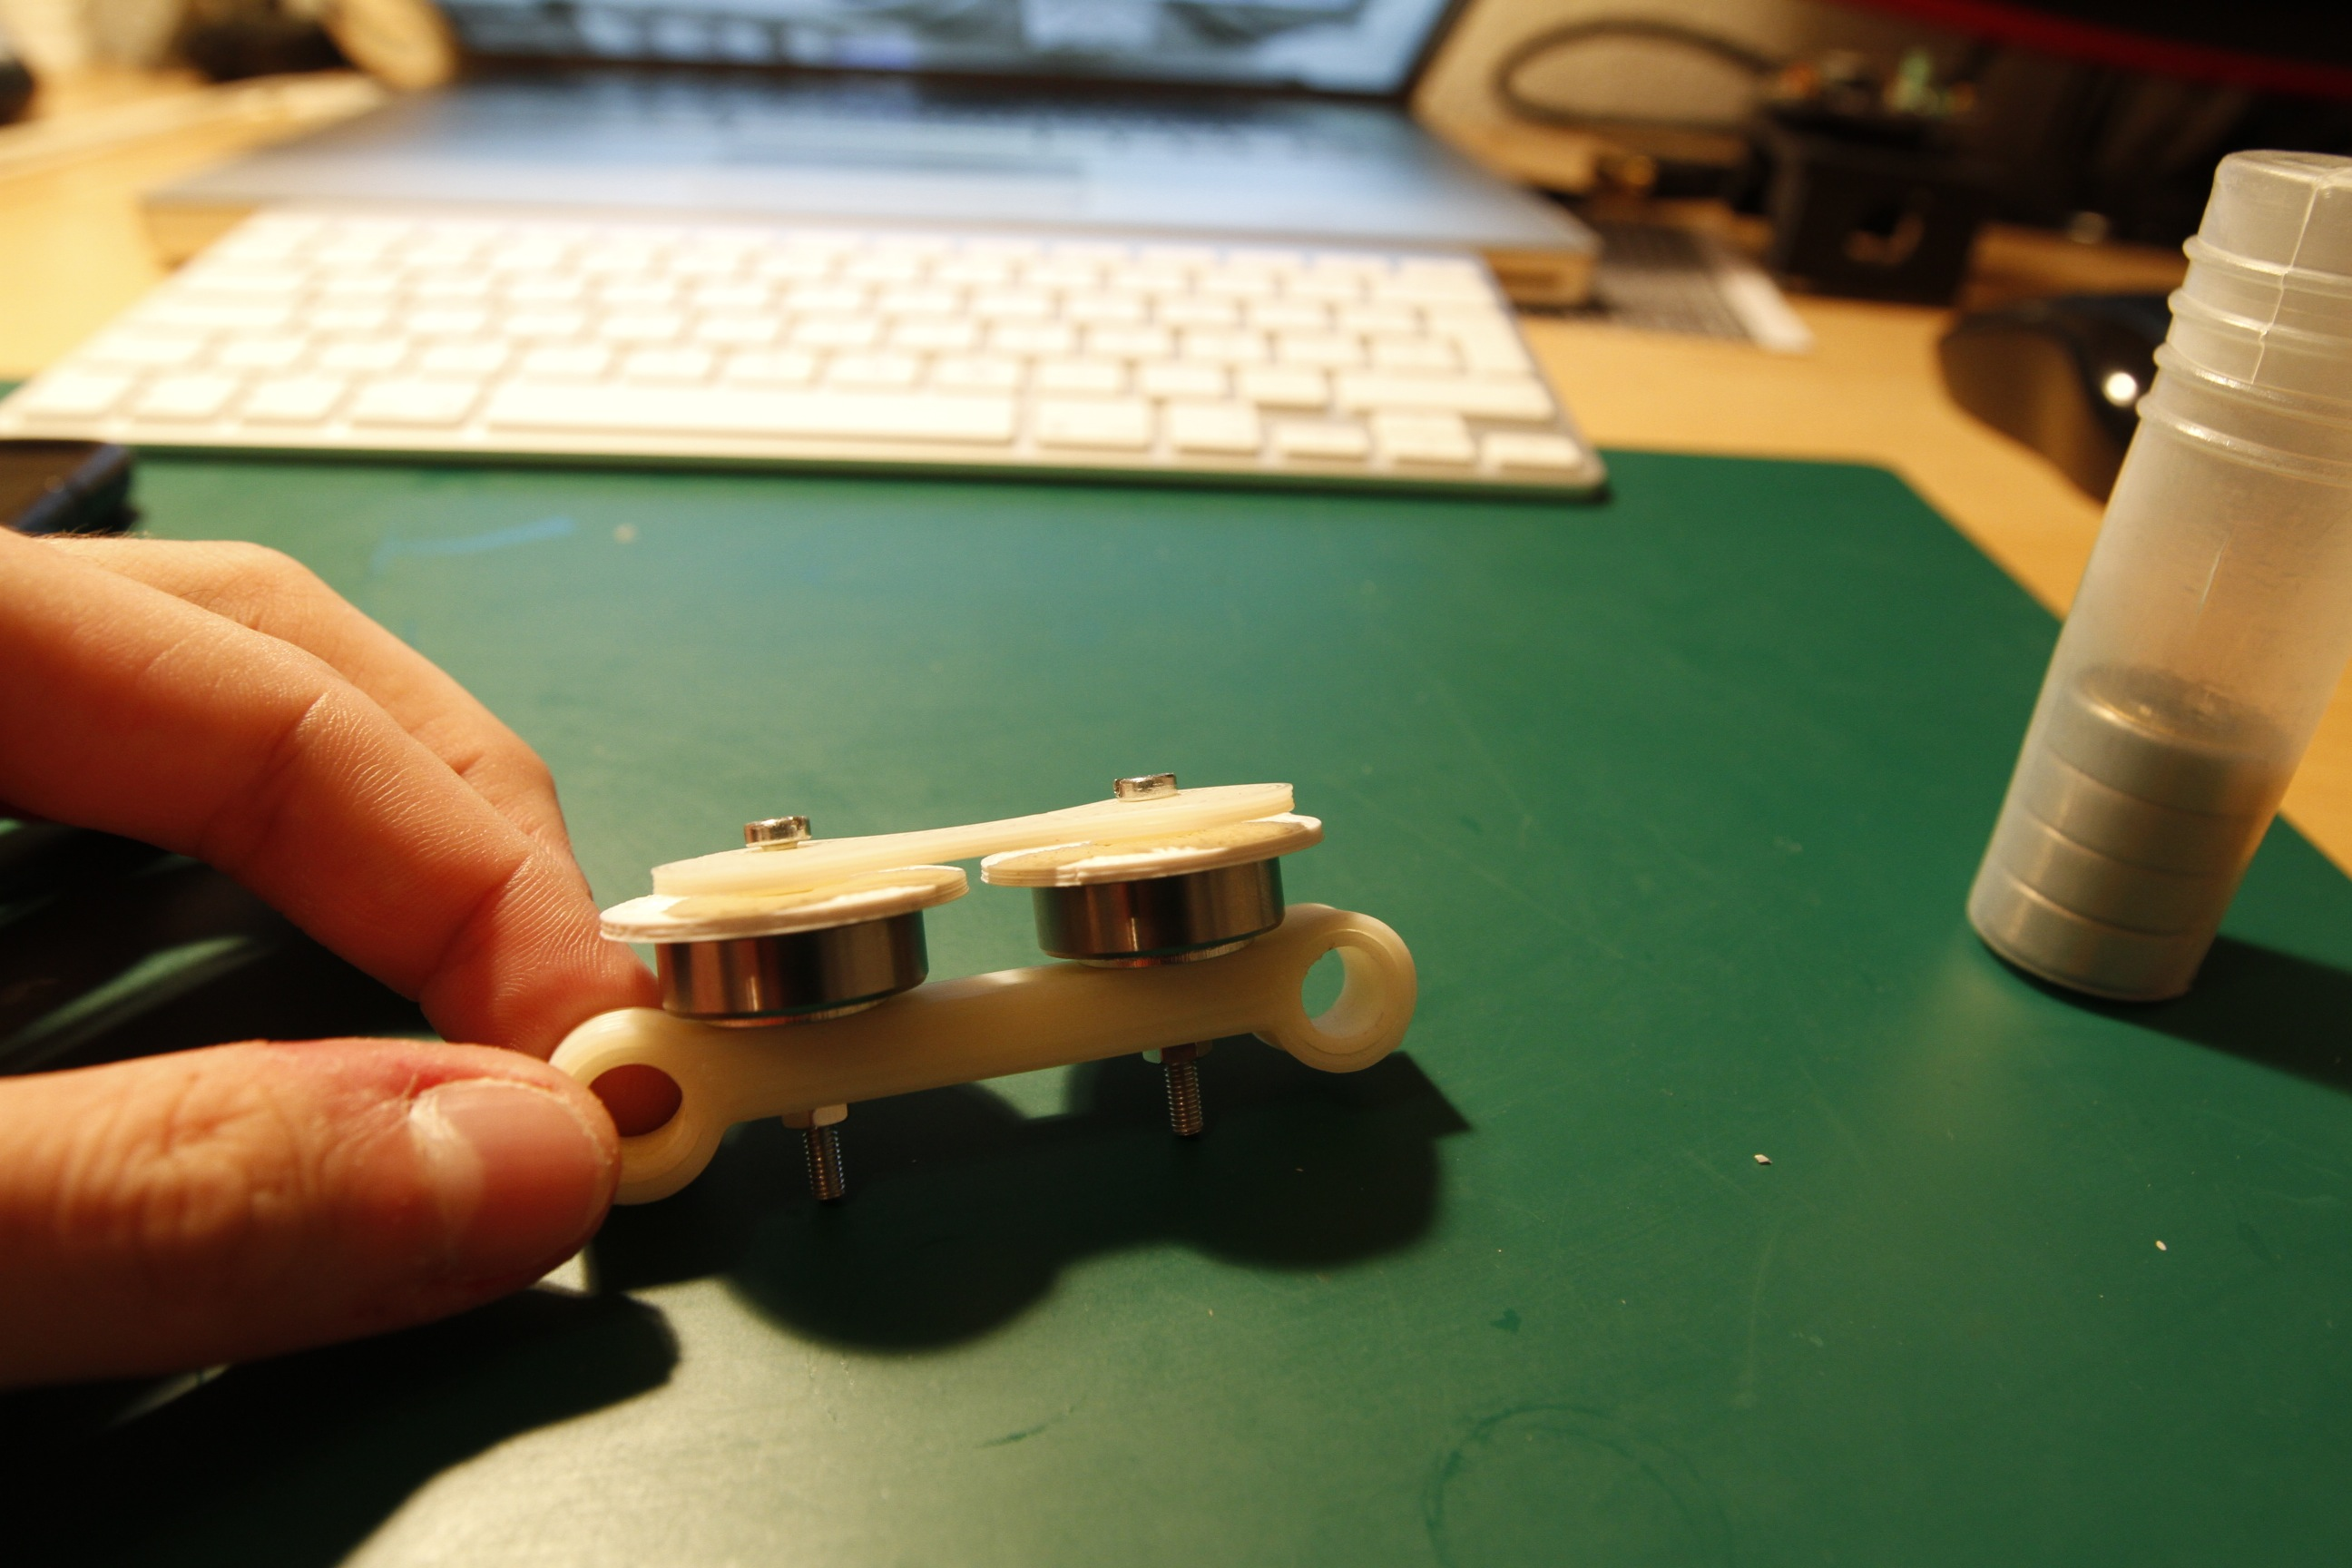
\includegraphics[width=\textwidth]{../../Fotos/71b.jpg}
		                %\caption{Distancia superior varillas lisas}
		                \label{fig:12.z}
		        \end{subfigure}
		        \caption{Bearing guide del eje Y}\label{fig:13.z}
		\end{figure}
		El siguiente paso será colocar los motores del eje Z como del eje Y; los del eje Z van a a los lados exteriores de la base, y el del eje Y va colocado en la parte interior derecha de la base, los atornillaremos con dos tornillos de M3x10 cada uno asegurándonos de que están correctamente apretados. En el motor dl eje Y colocaremos una polea dentada de T2.5 intentando que esté lo más pegada posible a la base del motor para a continuación colocar la rueda dentada. Volvemos a introducir el eje Y en los rodamientos lineales, para finalizar colocando la rueda dentada, El proceso se muestra en la figura ~\ref{fig:17.z}. Nos tenemos que asegurar que una vez colocada, la correa recorra la parte medía de la base de madera, para ello, desplazaremos en un sentido o en otro los rodamientos que hacen de guía a la correa.
		\begin{figure}[H]
		        \centering
		        \begin{subfigure}[htb]{0.5\textwidth}
		                \centering
		                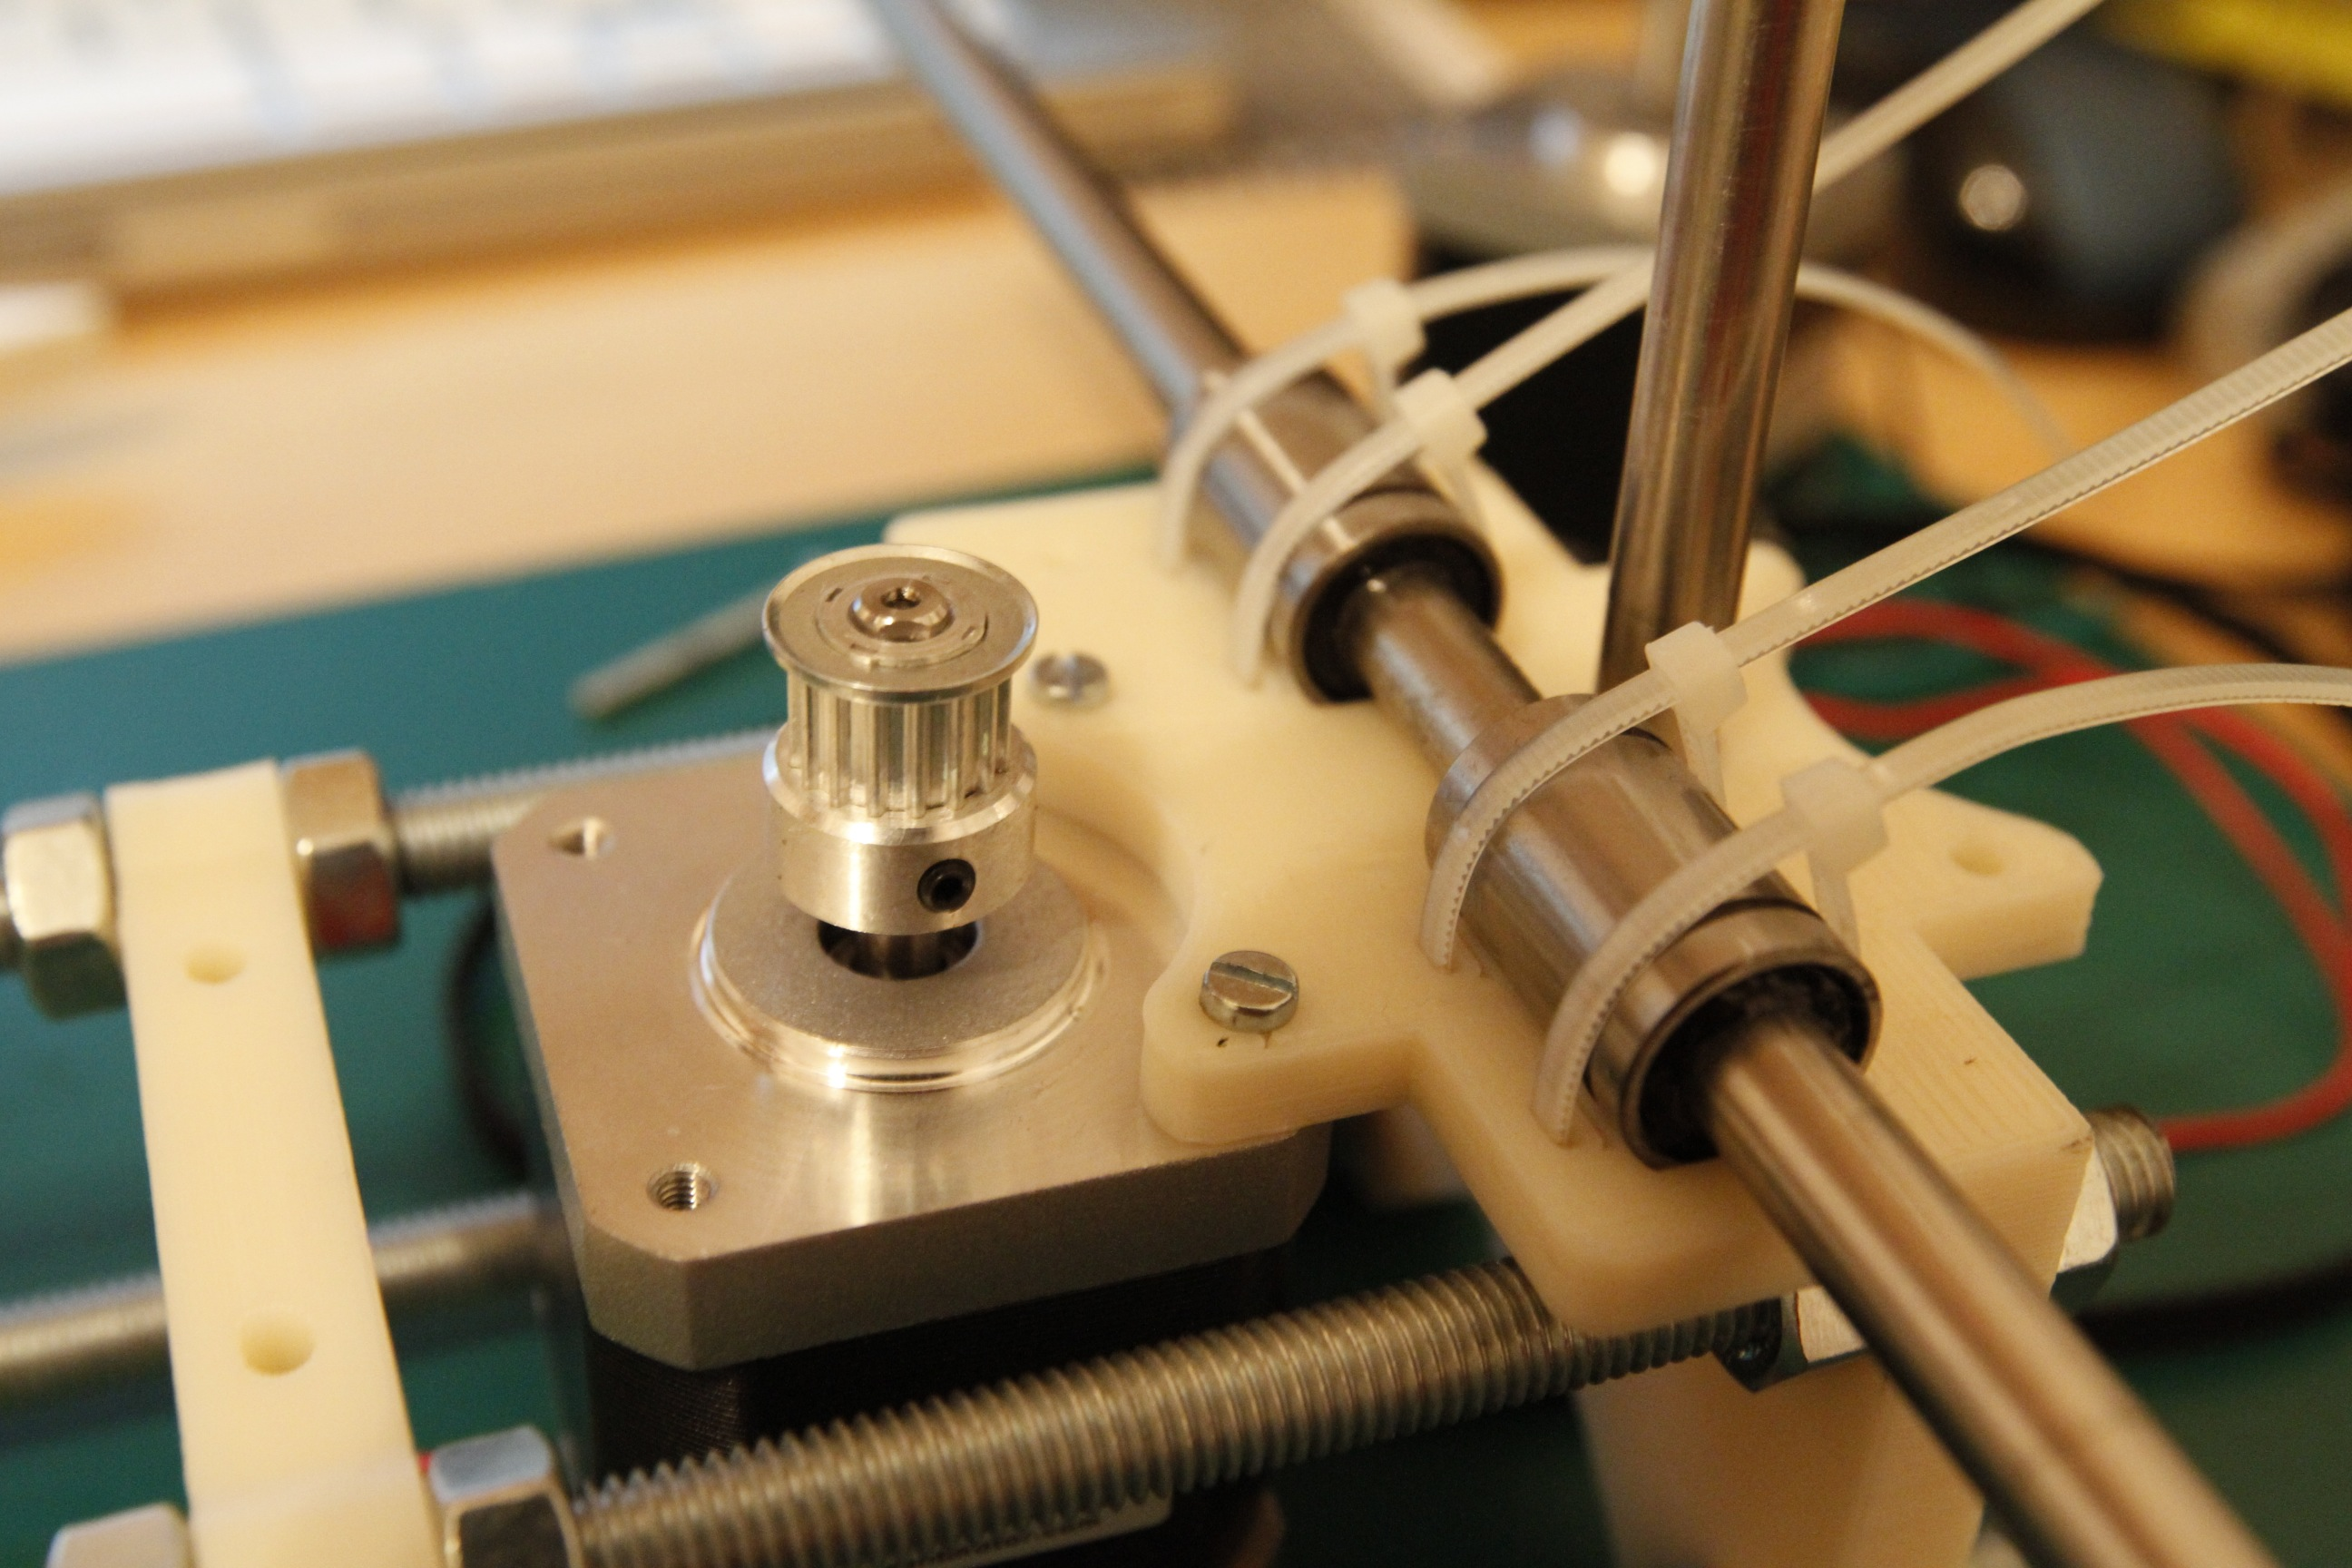
\includegraphics[width=\textwidth]{../../Fotos/80.jpg}
		                %\caption{Bearing Guide del eje Y}
		                \label{fig:14.z}
		        \end{subfigure}
		        \begin{subfigure}[htb]{0.5\textwidth}
		                \centering
		                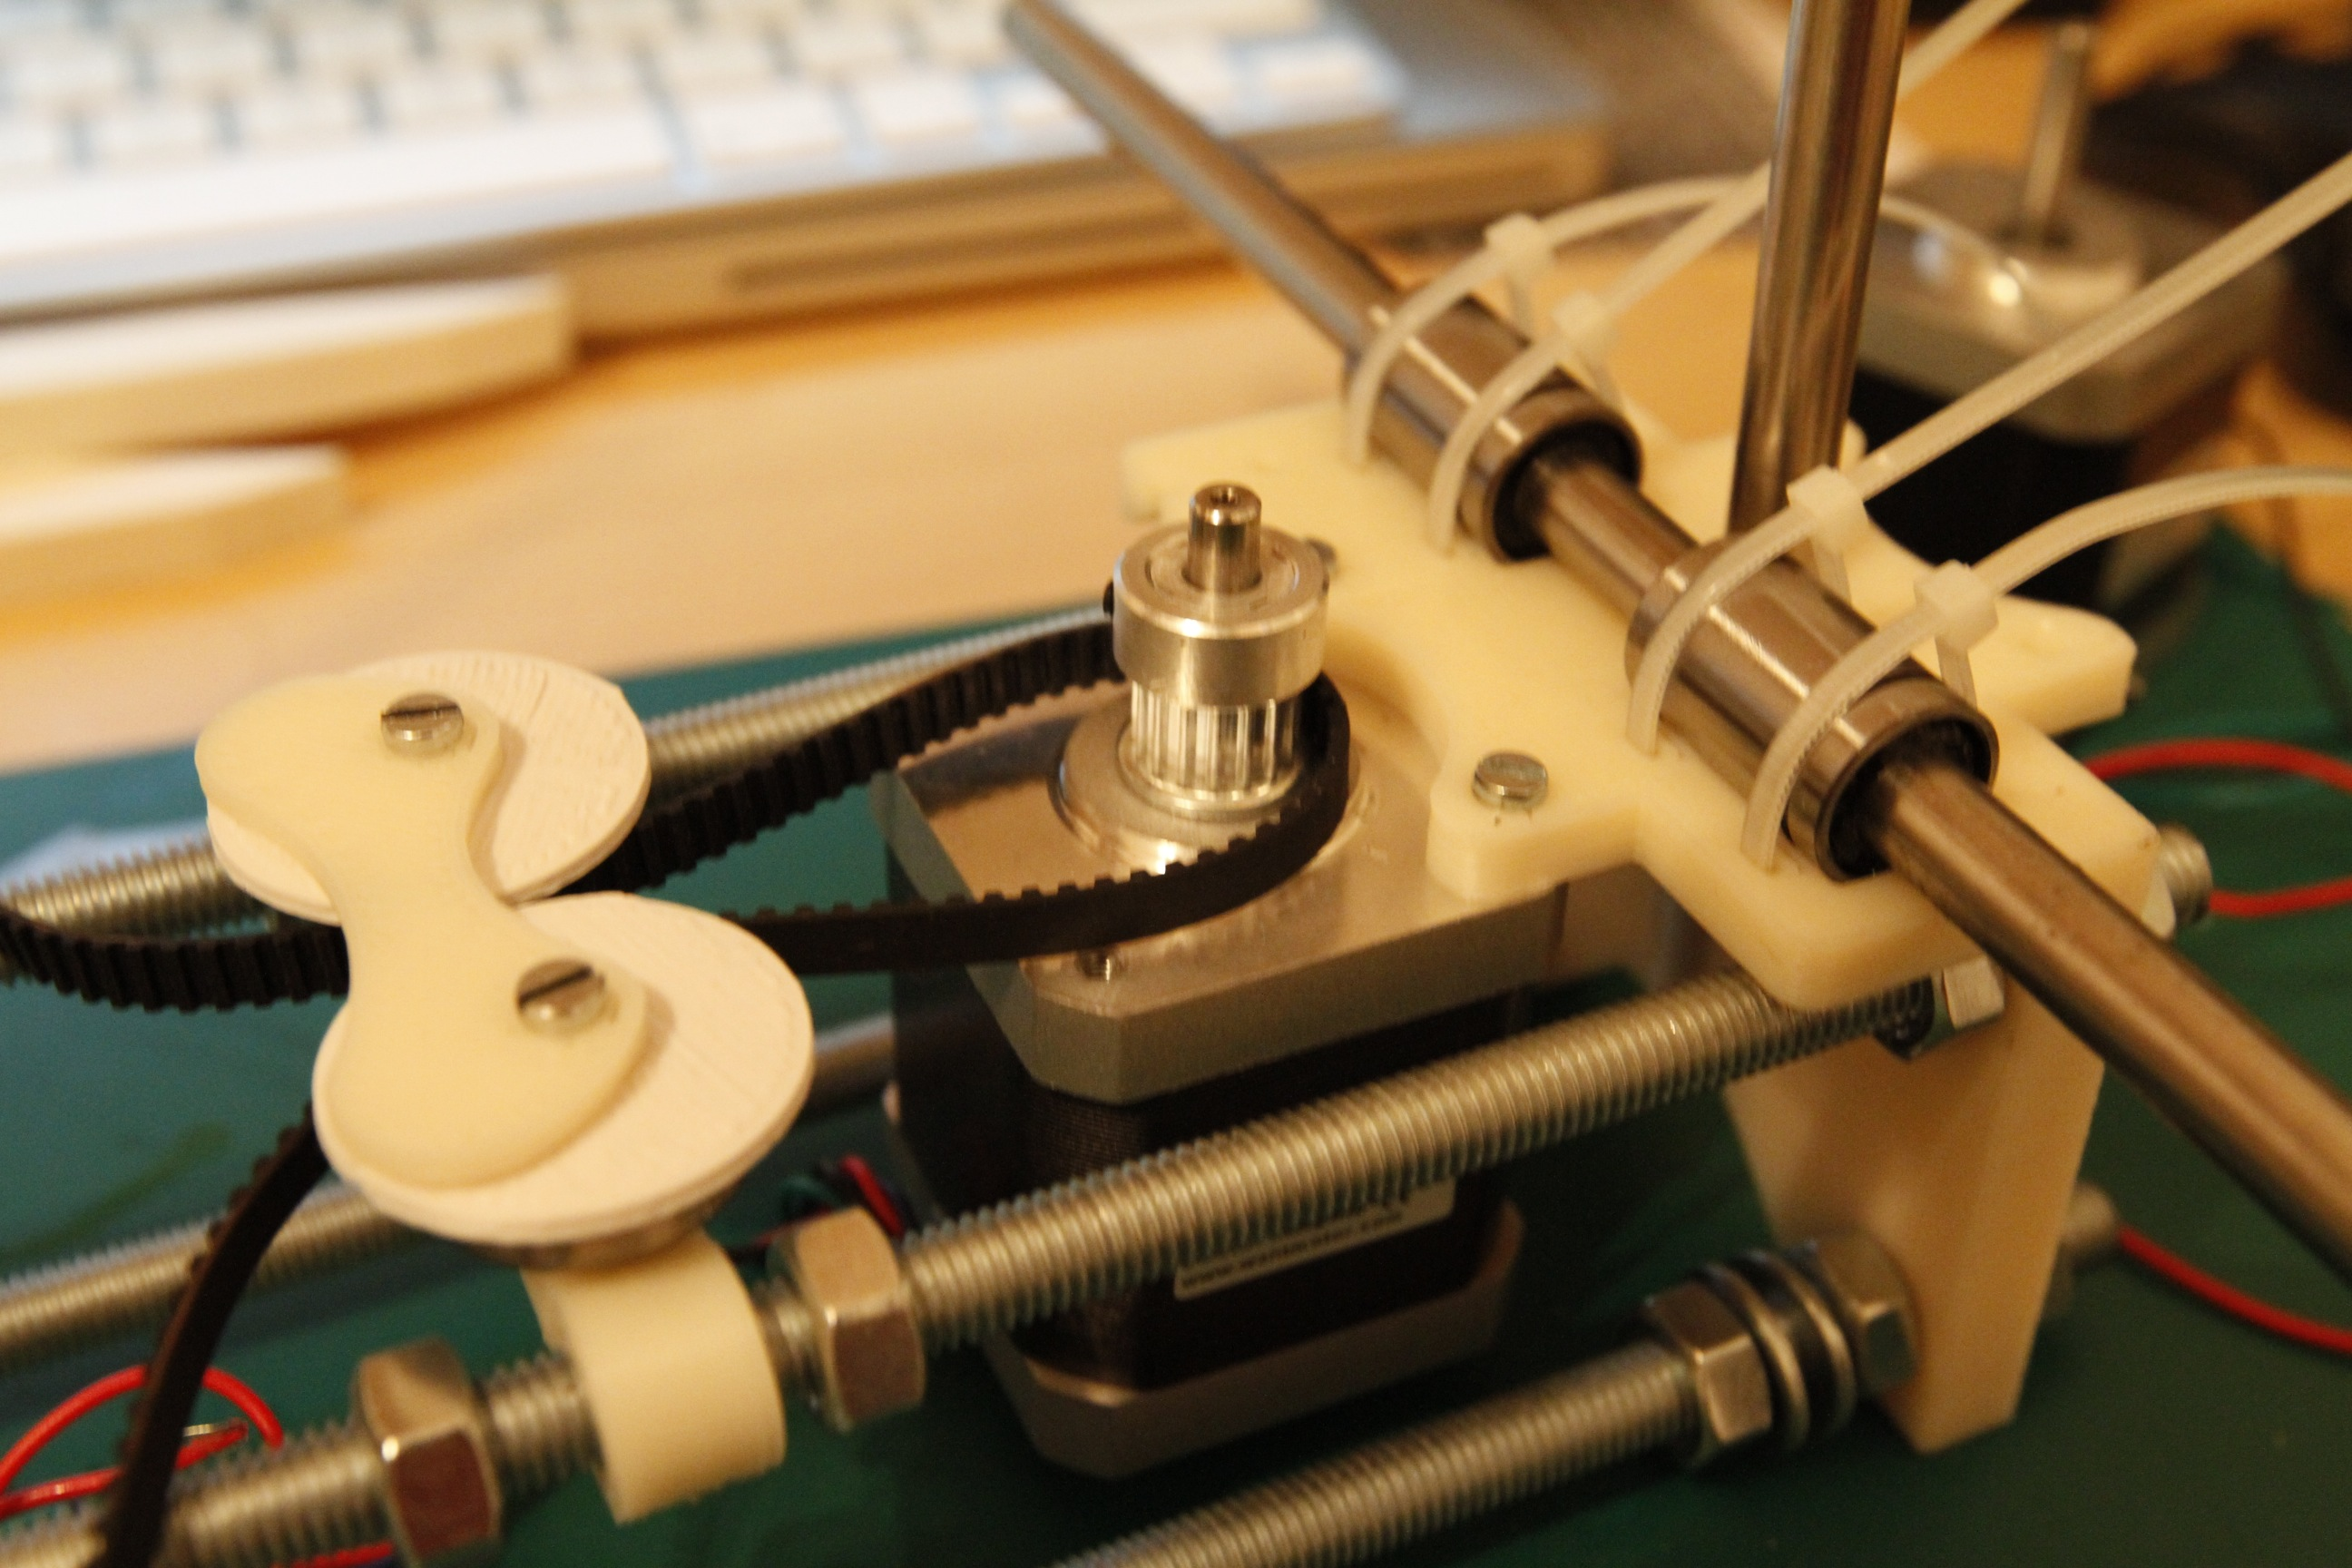
\includegraphics[width=\textwidth]{../../Fotos/81.jpg}
		                %\caption{Bearing Guide del eje Y}
		                \label{fig:15.z}
		        \end{subfigure}
		        \begin{subfigure}[htb]{0.5\textwidth}
		                \centering
		                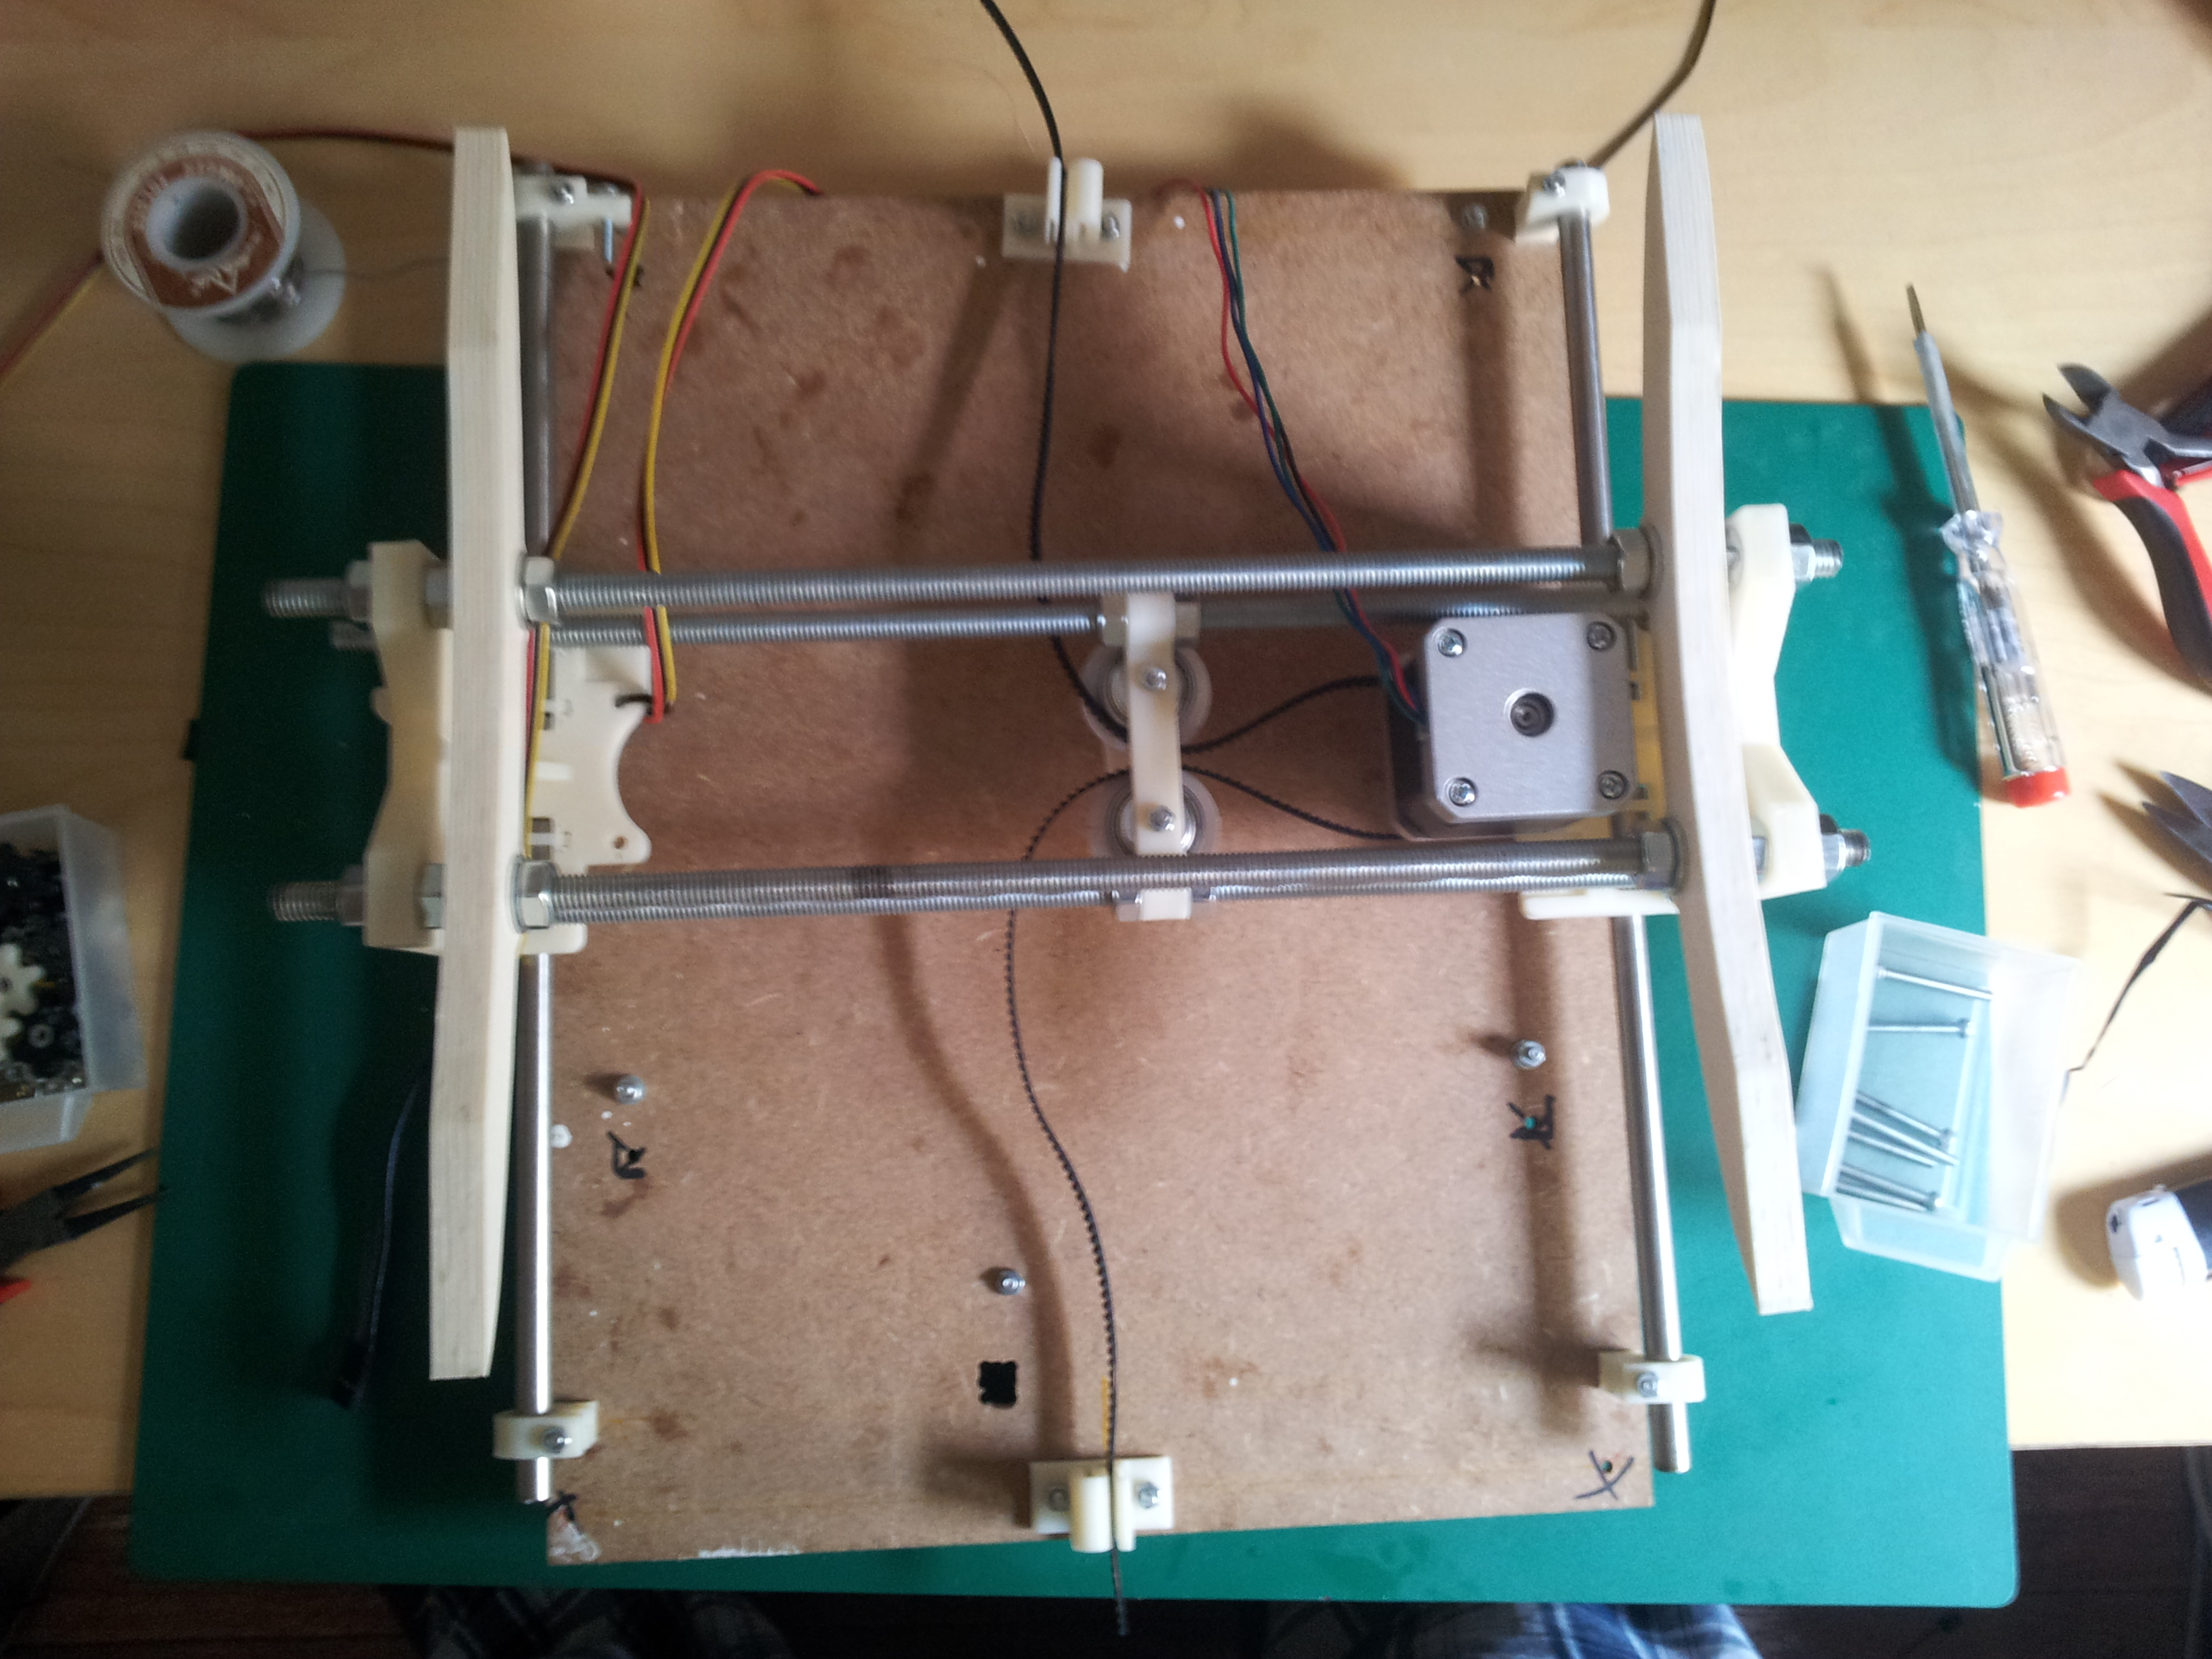
\includegraphics[width=\textwidth]{../../Fotos/82.jpg}
		                %\caption{Distancia superior varillas lisas}
		                \label{fig:16.z}
		        \end{subfigure}
		        \caption{Colocando el eje Y}\label{fig:17.z}
		\end{figure}
		Una vez presentada la correa, la apretaremos a las piezas del eje Y con la ayuda de una brida como se muestra a continuación:
		\begin{figure}[!htp]
			\centering
			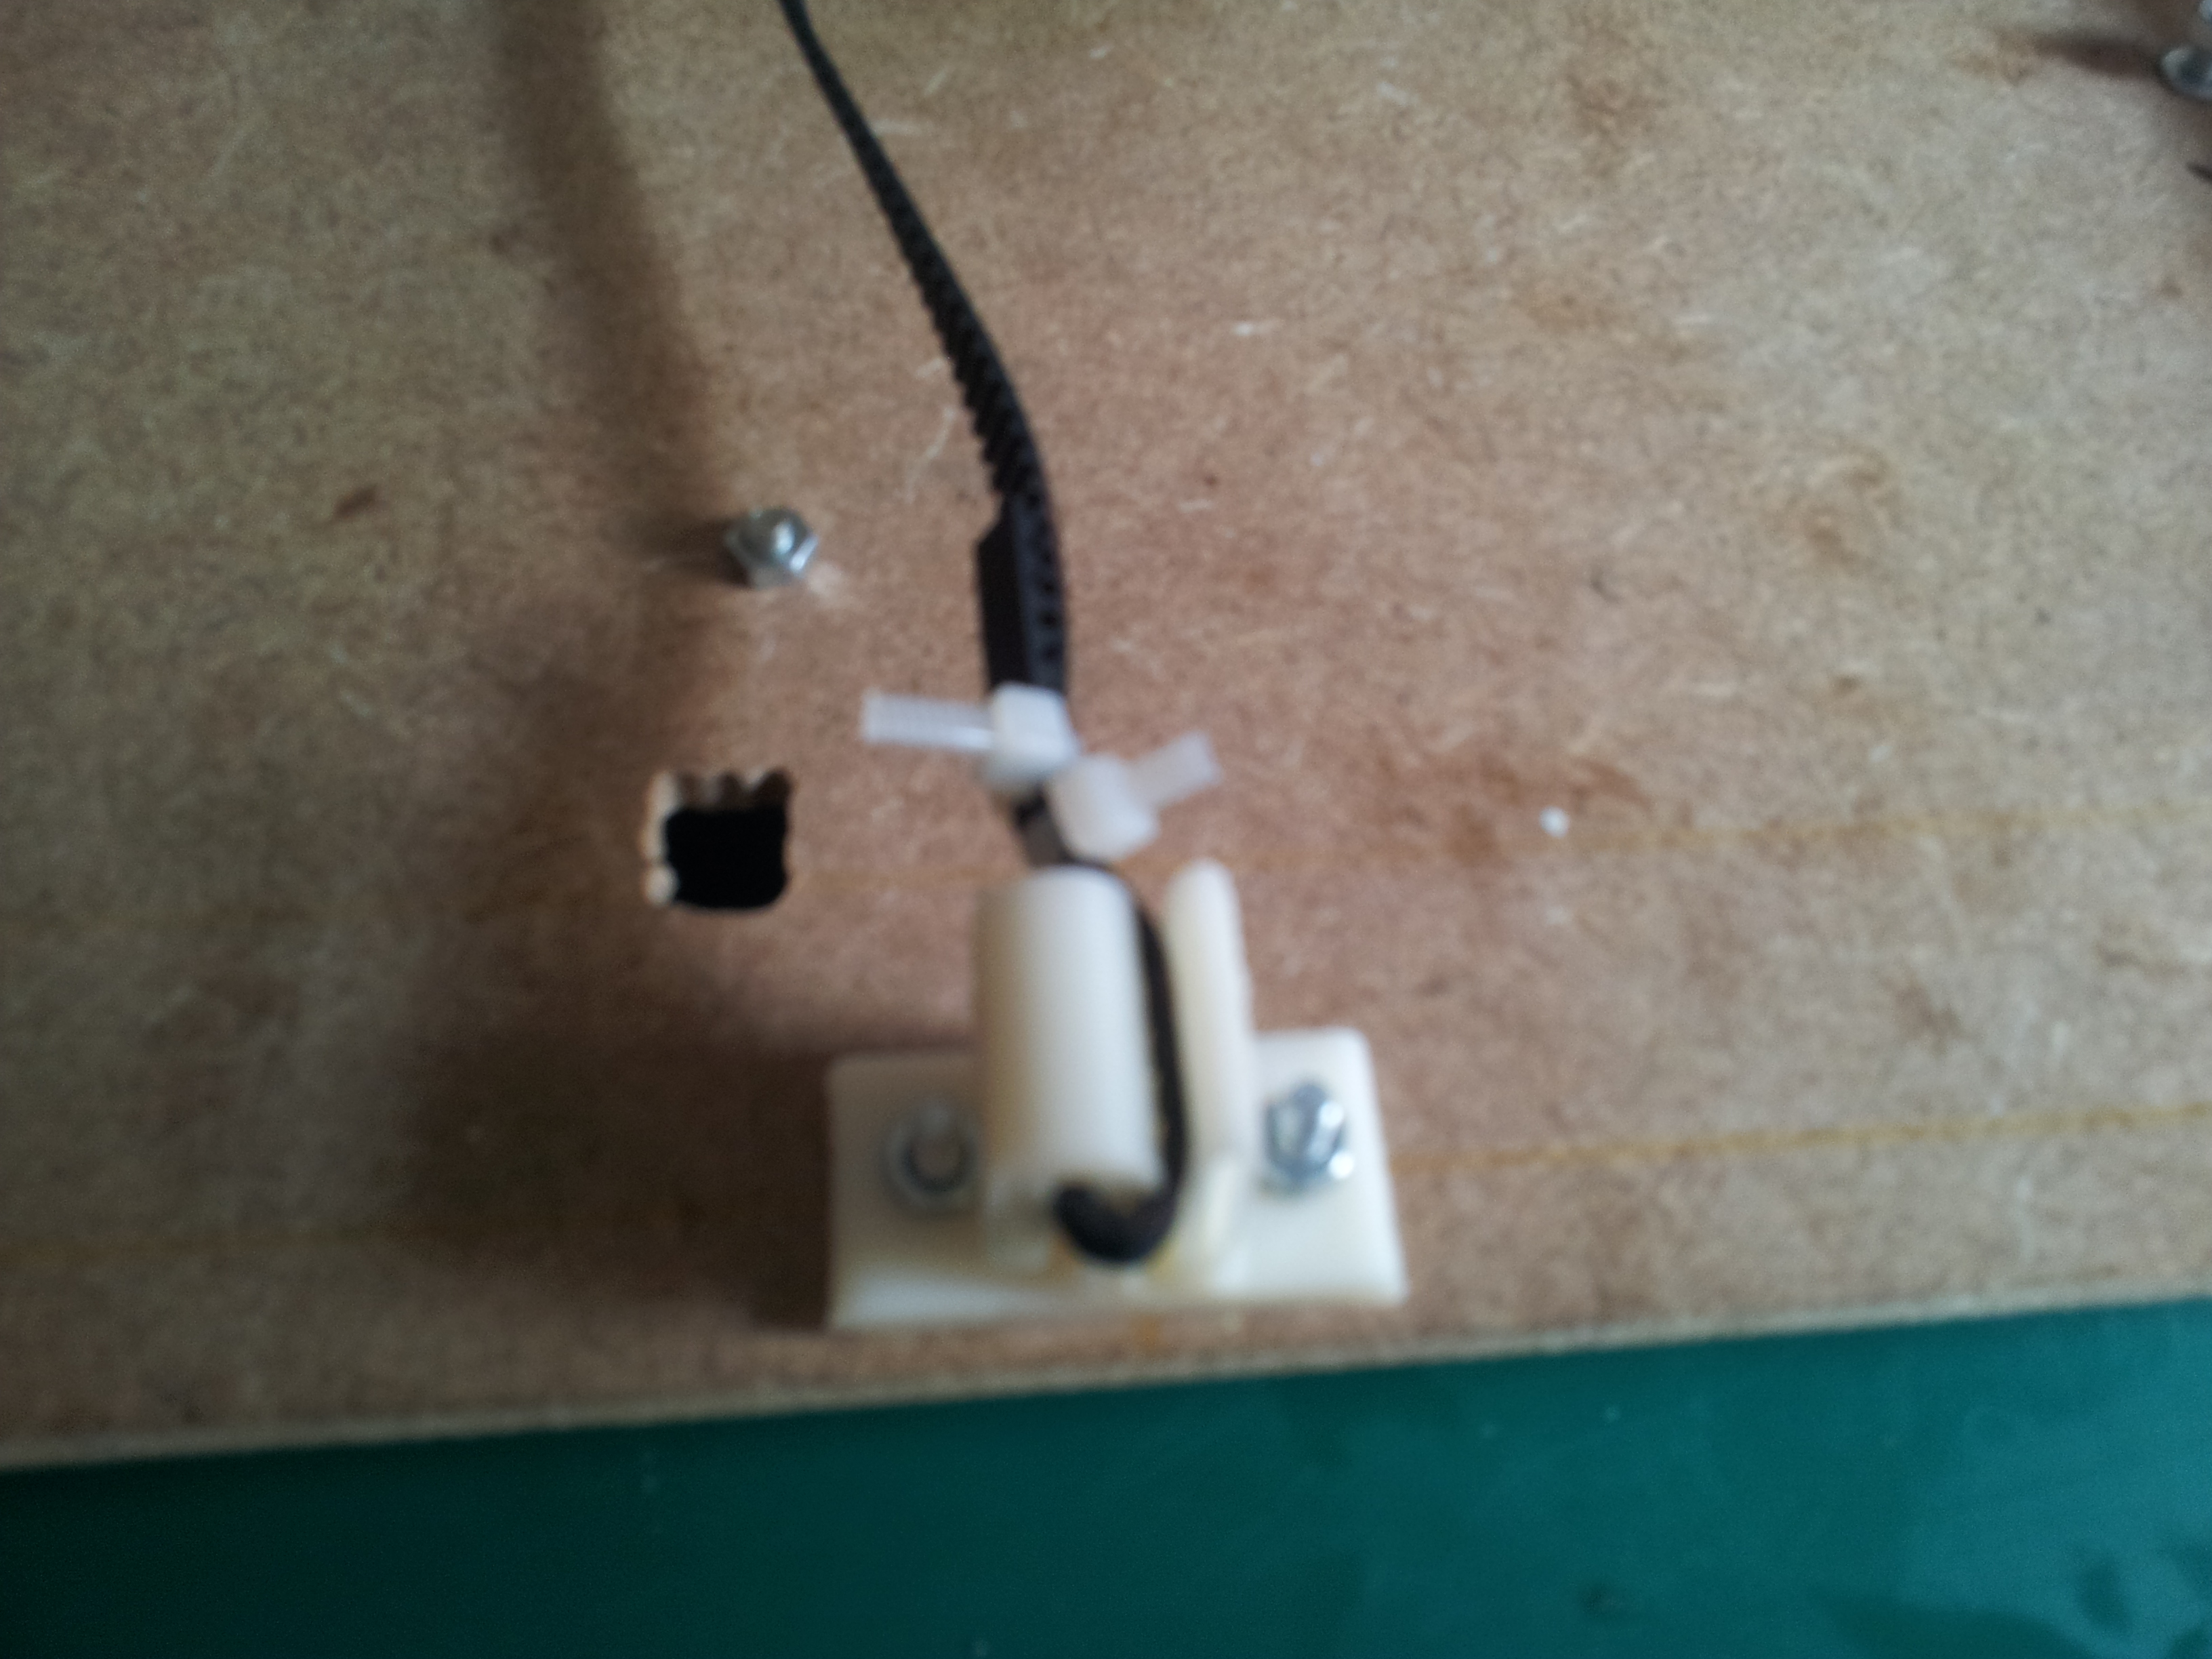
\includegraphics[width=0.6\textwidth]{../../Fotos/83.jpg}
			\caption{Correa del eje Y}
			\label{fig:18.z}
		\end{figure}
		Una vez que comprobamos que el eje Y es capaz de desplazar correctamente con la mano apretaremos las bridas de los rodamientos lineales situados en la base del eje Z.\\
		Pasaremos ahora a modificar las piezas para sujetar el vástago de los motores a las varillas roscadas del eje Z. Para ello deberemos hacer pasantes los agujeros que se indican en las figuras, con ayuda de un cutter y una lima de 3mm. ~\ref{fig:21.z}
		\begin{figure}[H]
		        \centering
		        \begin{subfigure}[htb]{0.5\textwidth}
		                \centering
		                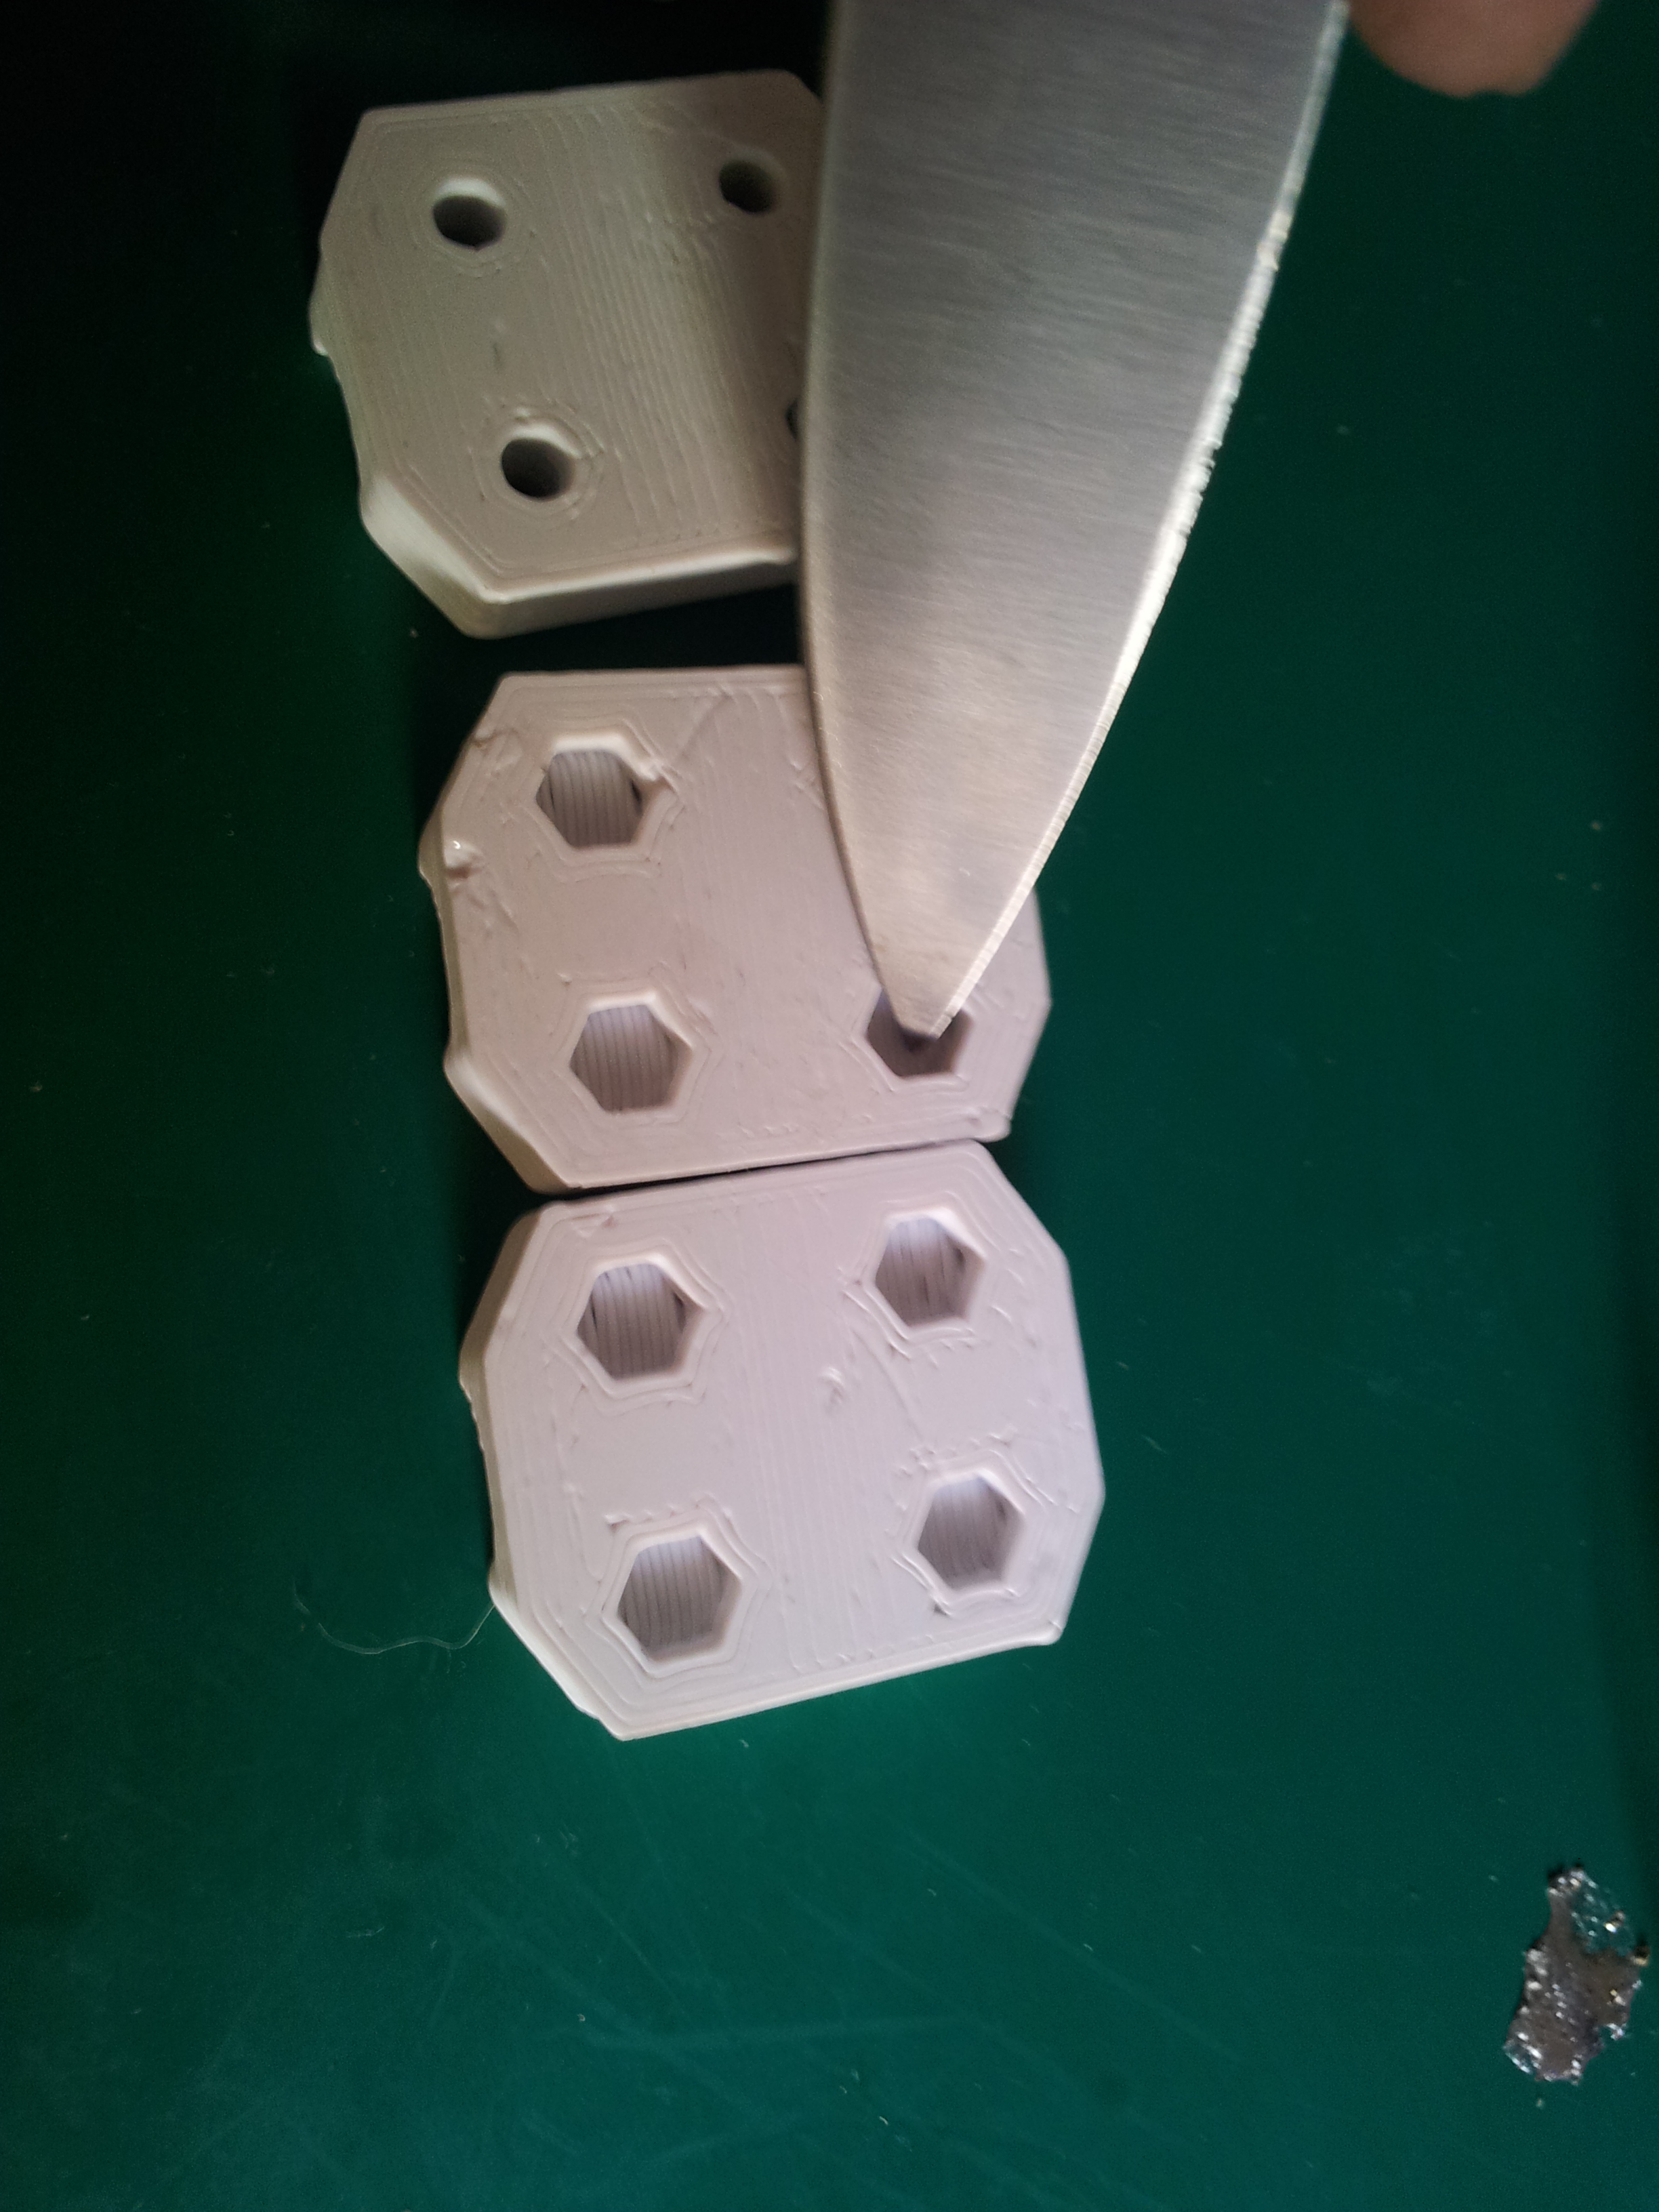
\includegraphics[width=\textwidth]{../../Fotos/87.jpg}
		                %\caption{Bearing Guide del eje Y}
		                \label{fig:19.z}
		        \end{subfigure}
		        \begin{subfigure}[htb]{0.5\textwidth}
		                \centering
		                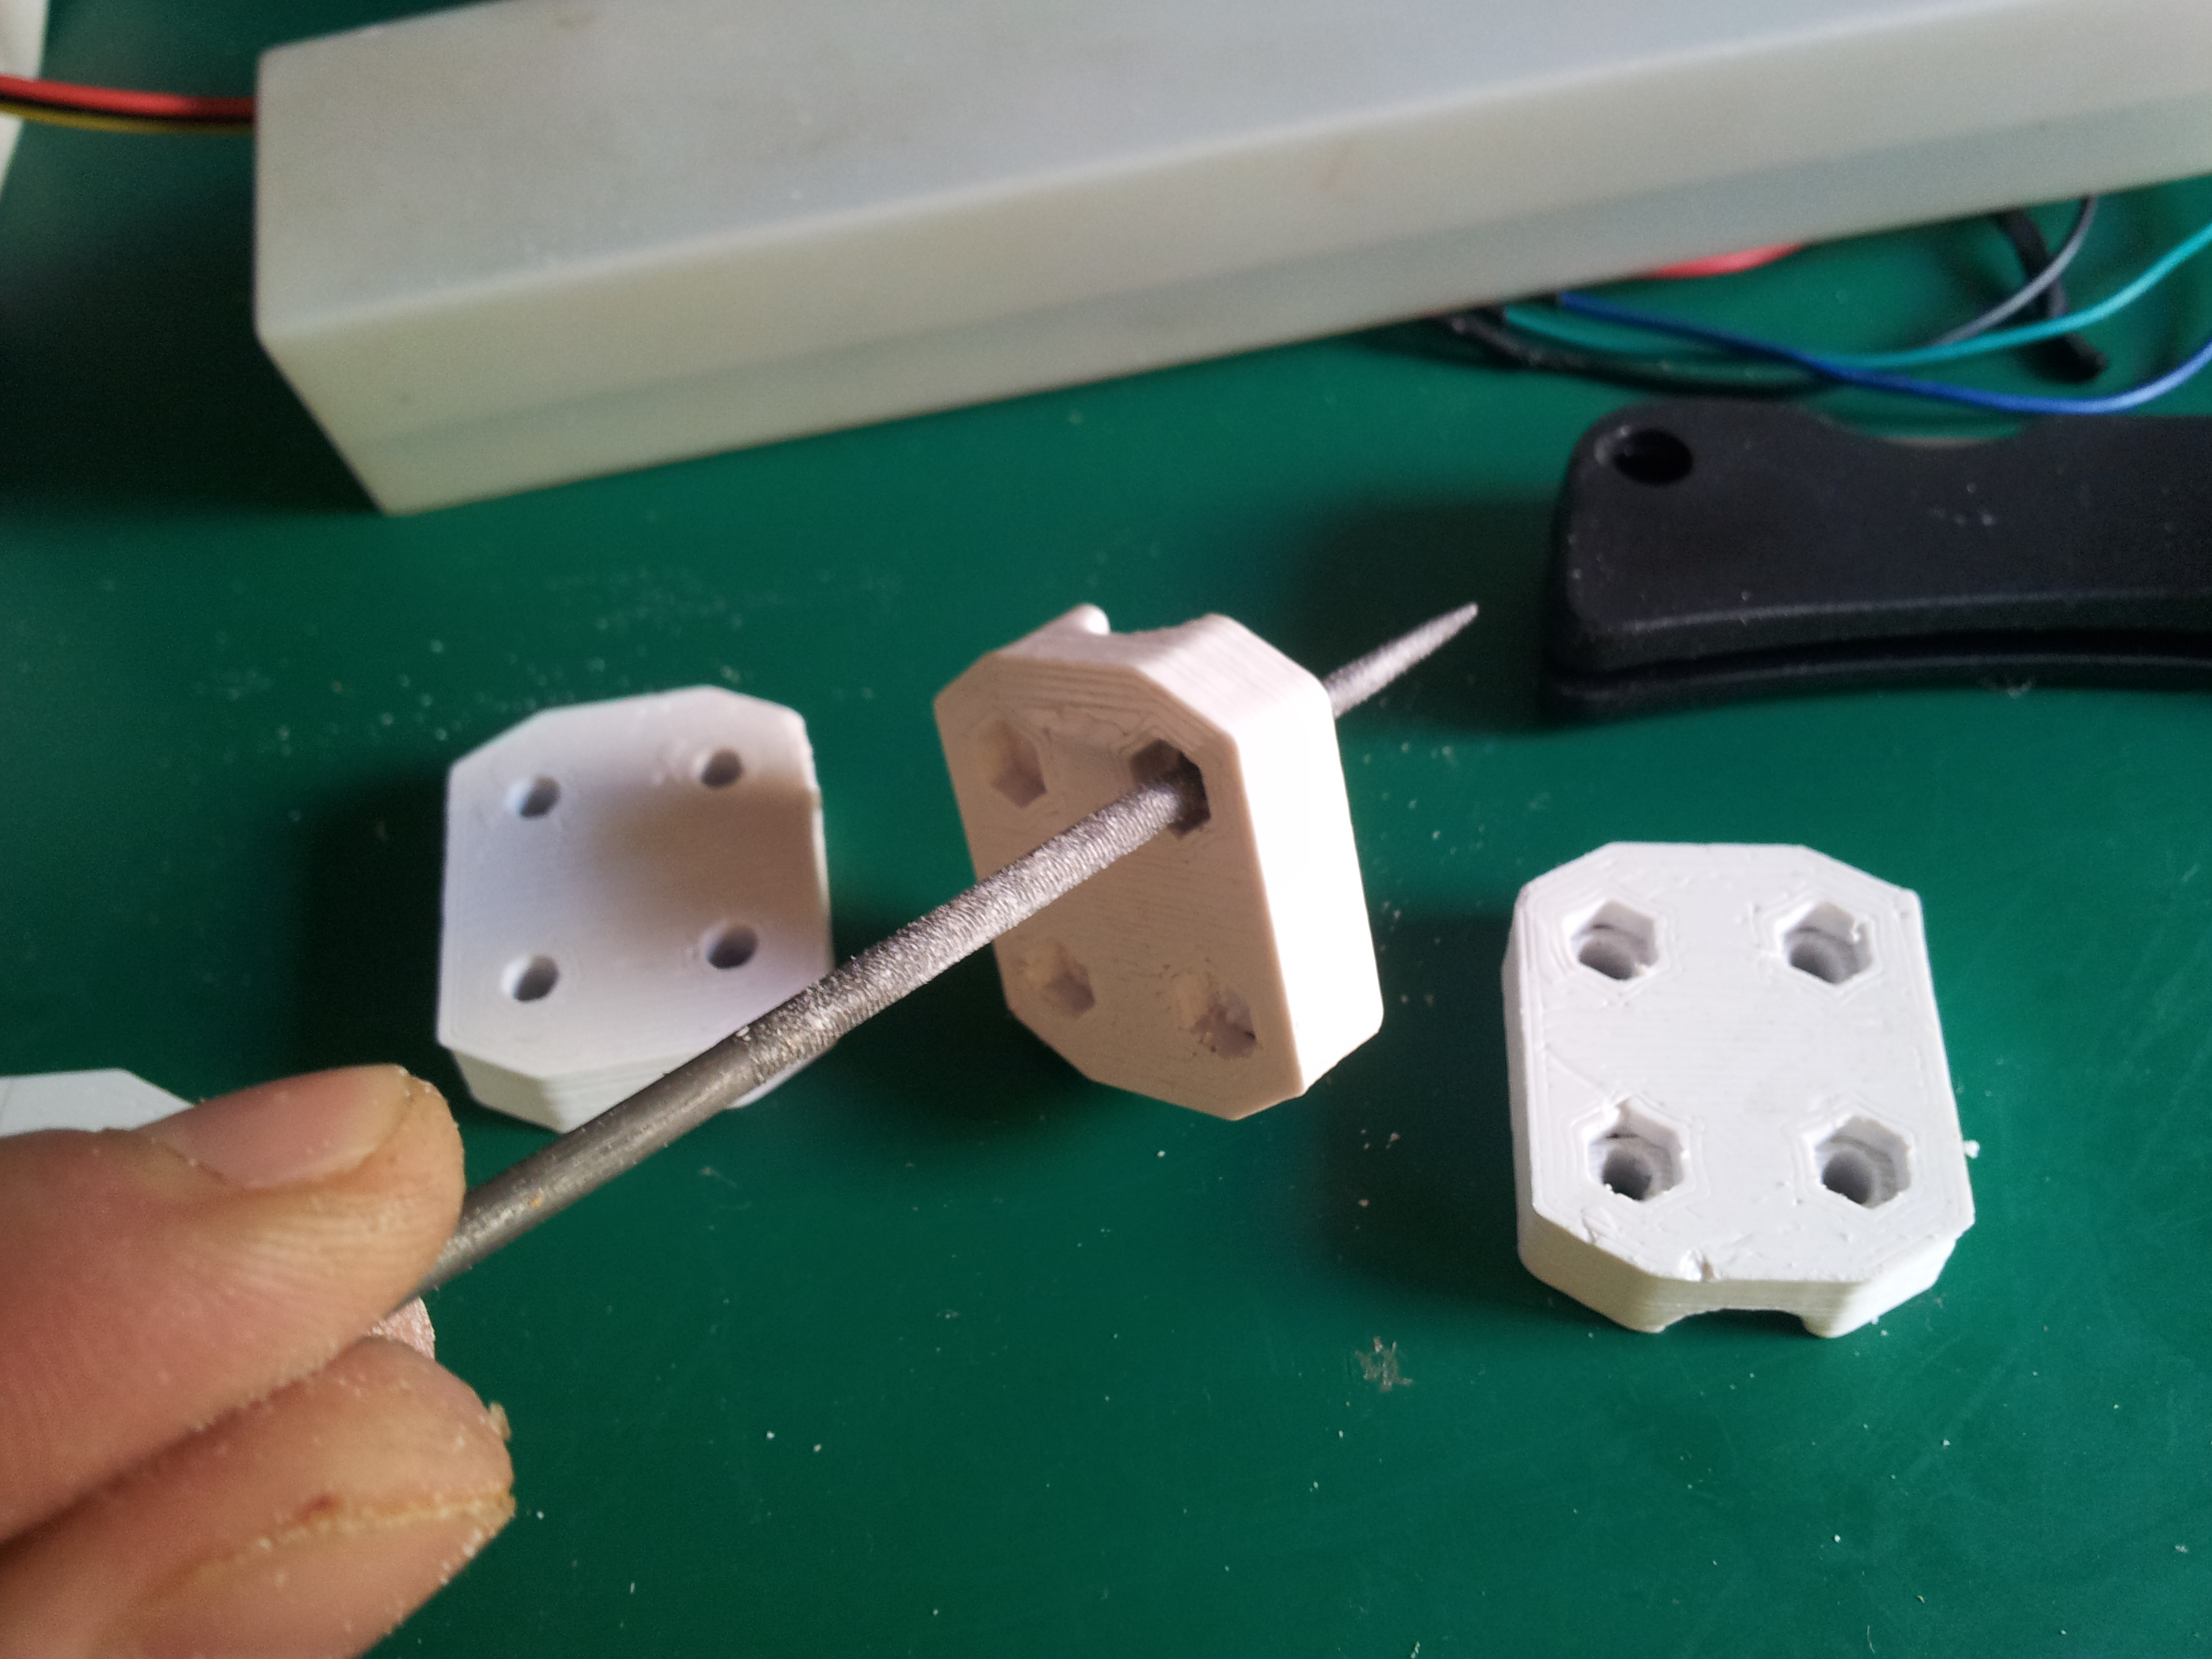
\includegraphics[width=\textwidth]{../../Fotos/88.jpg}
		                %\caption{Bearing Guide del eje Y}
		                \label{fig:120.z}
		        \end{subfigure}
		        \caption{Modificando piezas Z coupling}\label{fig:21.z}
		\end{figure}
		una vez hechos los agujeros pasantes, deberemos empotrar las tuercas de M3 en los agujeros destinados a ello, mediante un soldador y aplicando calor a la tuerca, las empotramos.
		Para finalizar, introducimos un poco de tubo de pecera en el vástago del motor del eje Z y colocamos la varilla roscada, asegurandonos que queda totalmente recta con ayuda de los z coupling.
		\begin{figure}[!htp]
			\centering
	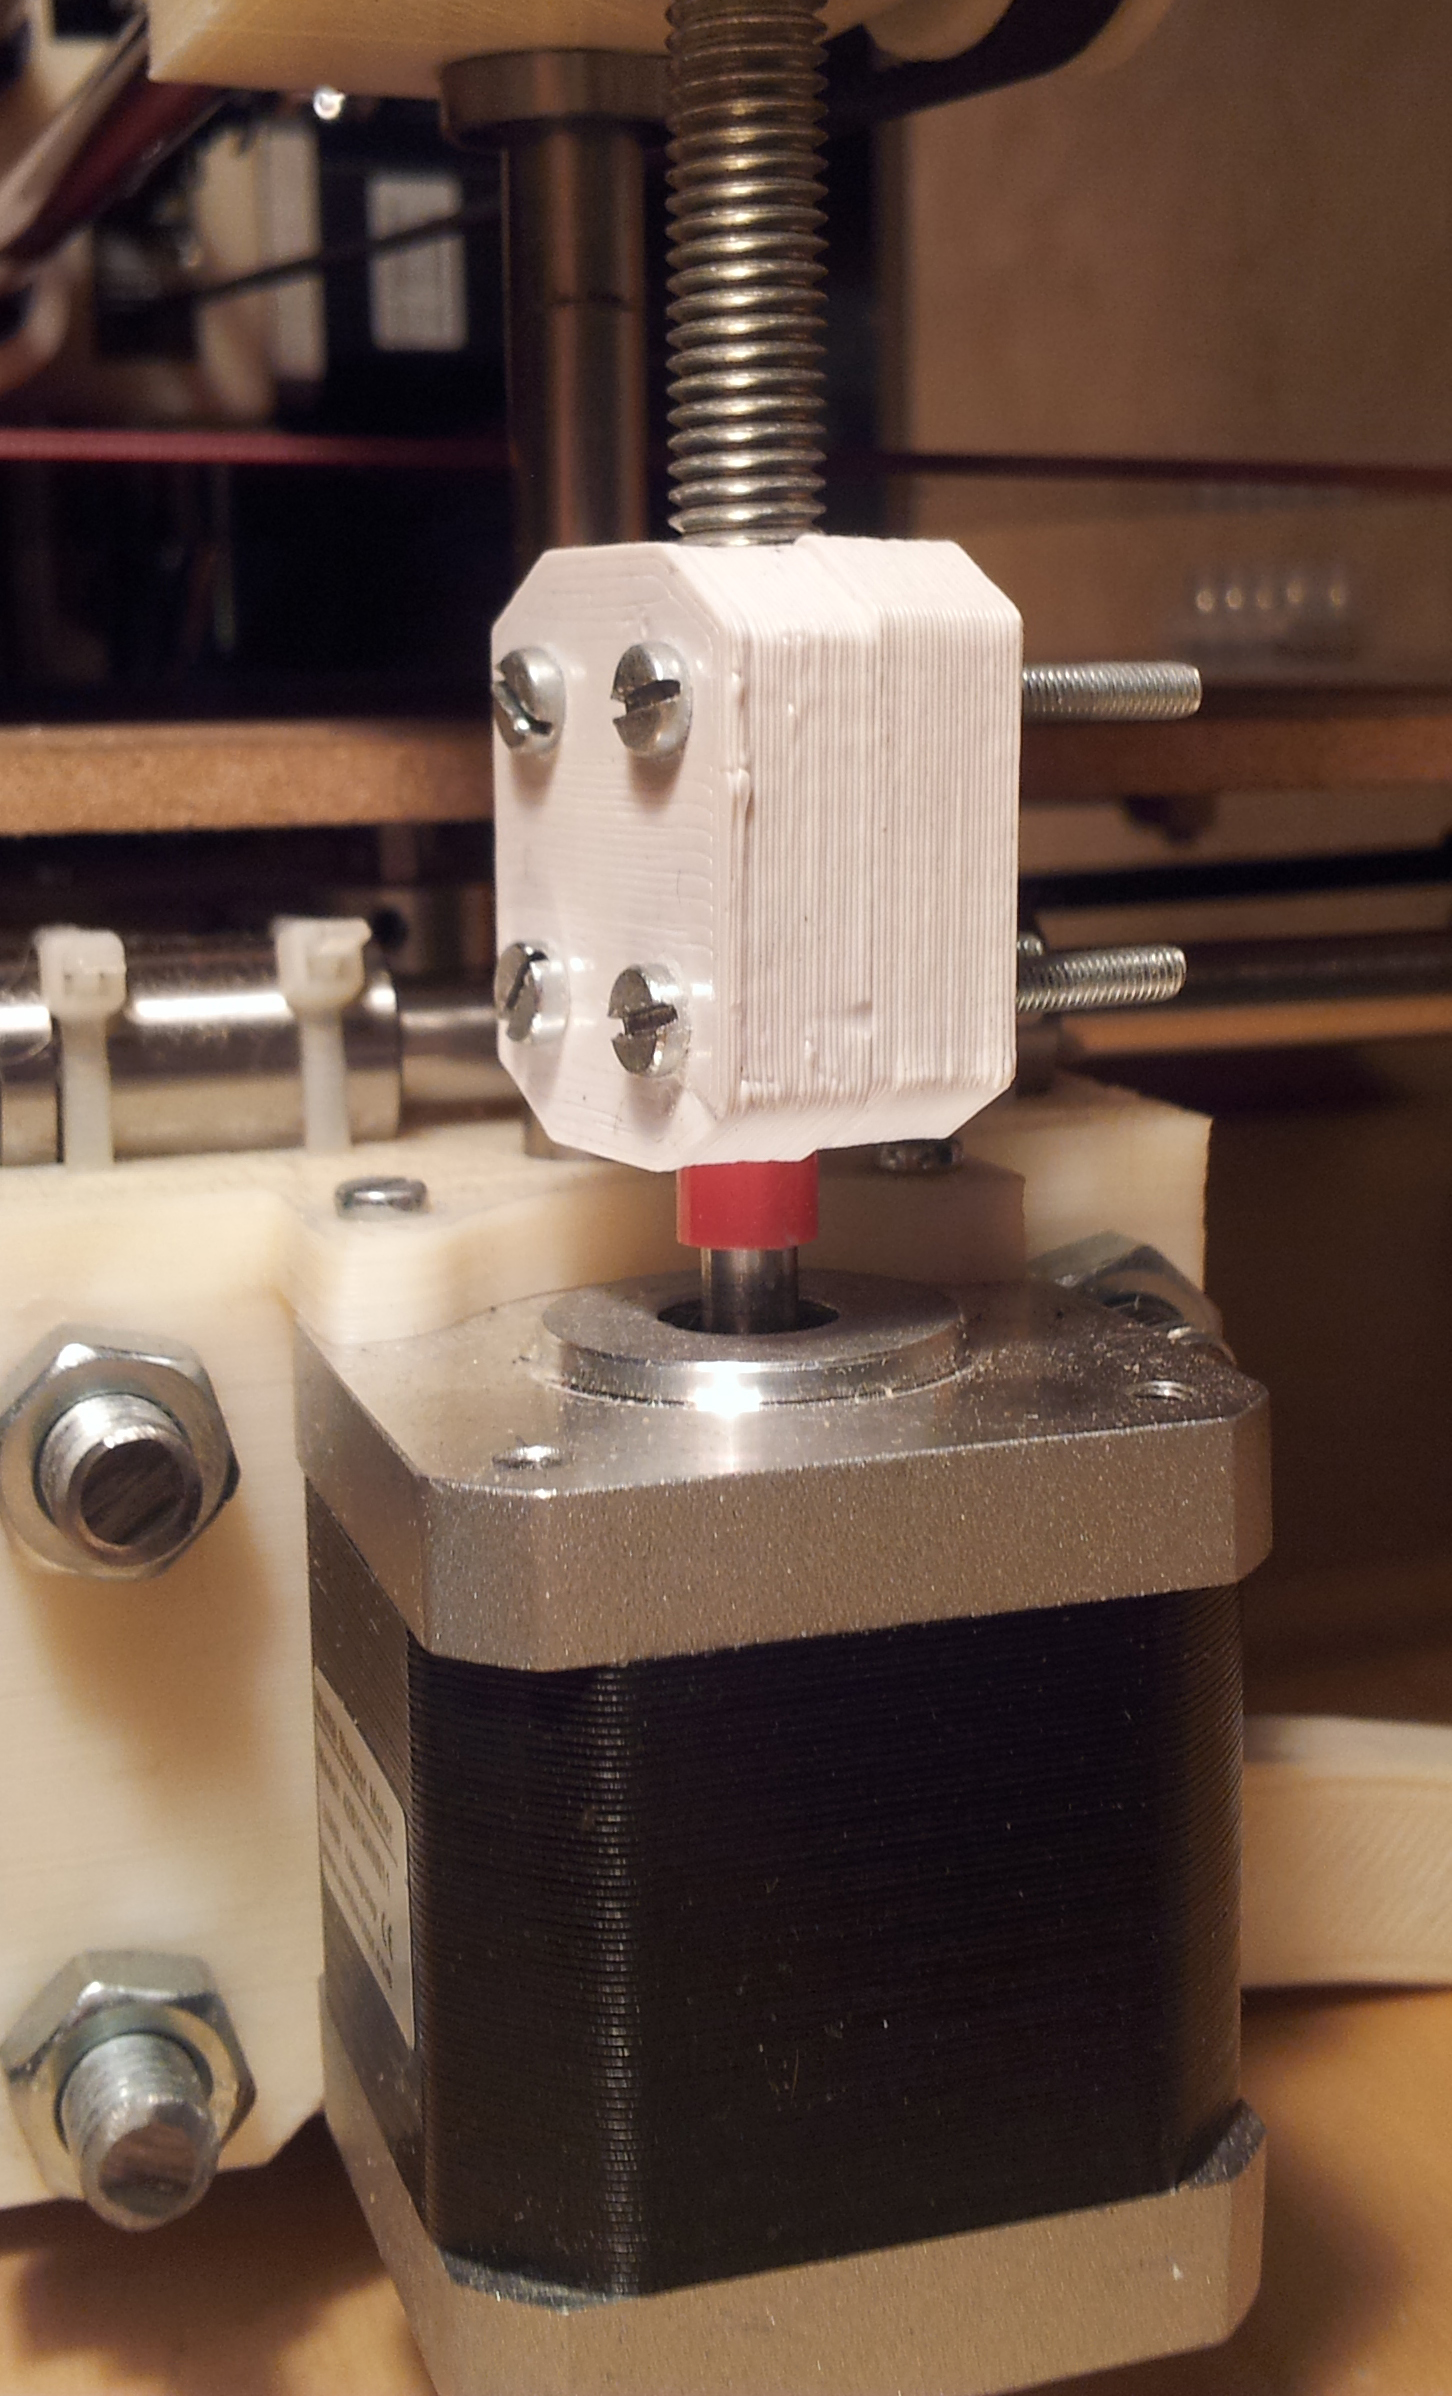
\includegraphics[width=0.6\textwidth]{../../Fotos/93.jpg}
			\caption{Varilla roscada en vástgago de motor}
			\label{fig:24.z}
		\end{figure}
		Como último paso, podremos introducir ya el eje X a través de las varillas roscadas y las varillas lisas como se puede ver en la figura ~\ref{fig:23.z}\\
		
		\begin{figure}[H]
		        \centering
		        \begin{subfigure}[htb]{0.5\textwidth}
		                \centering
		                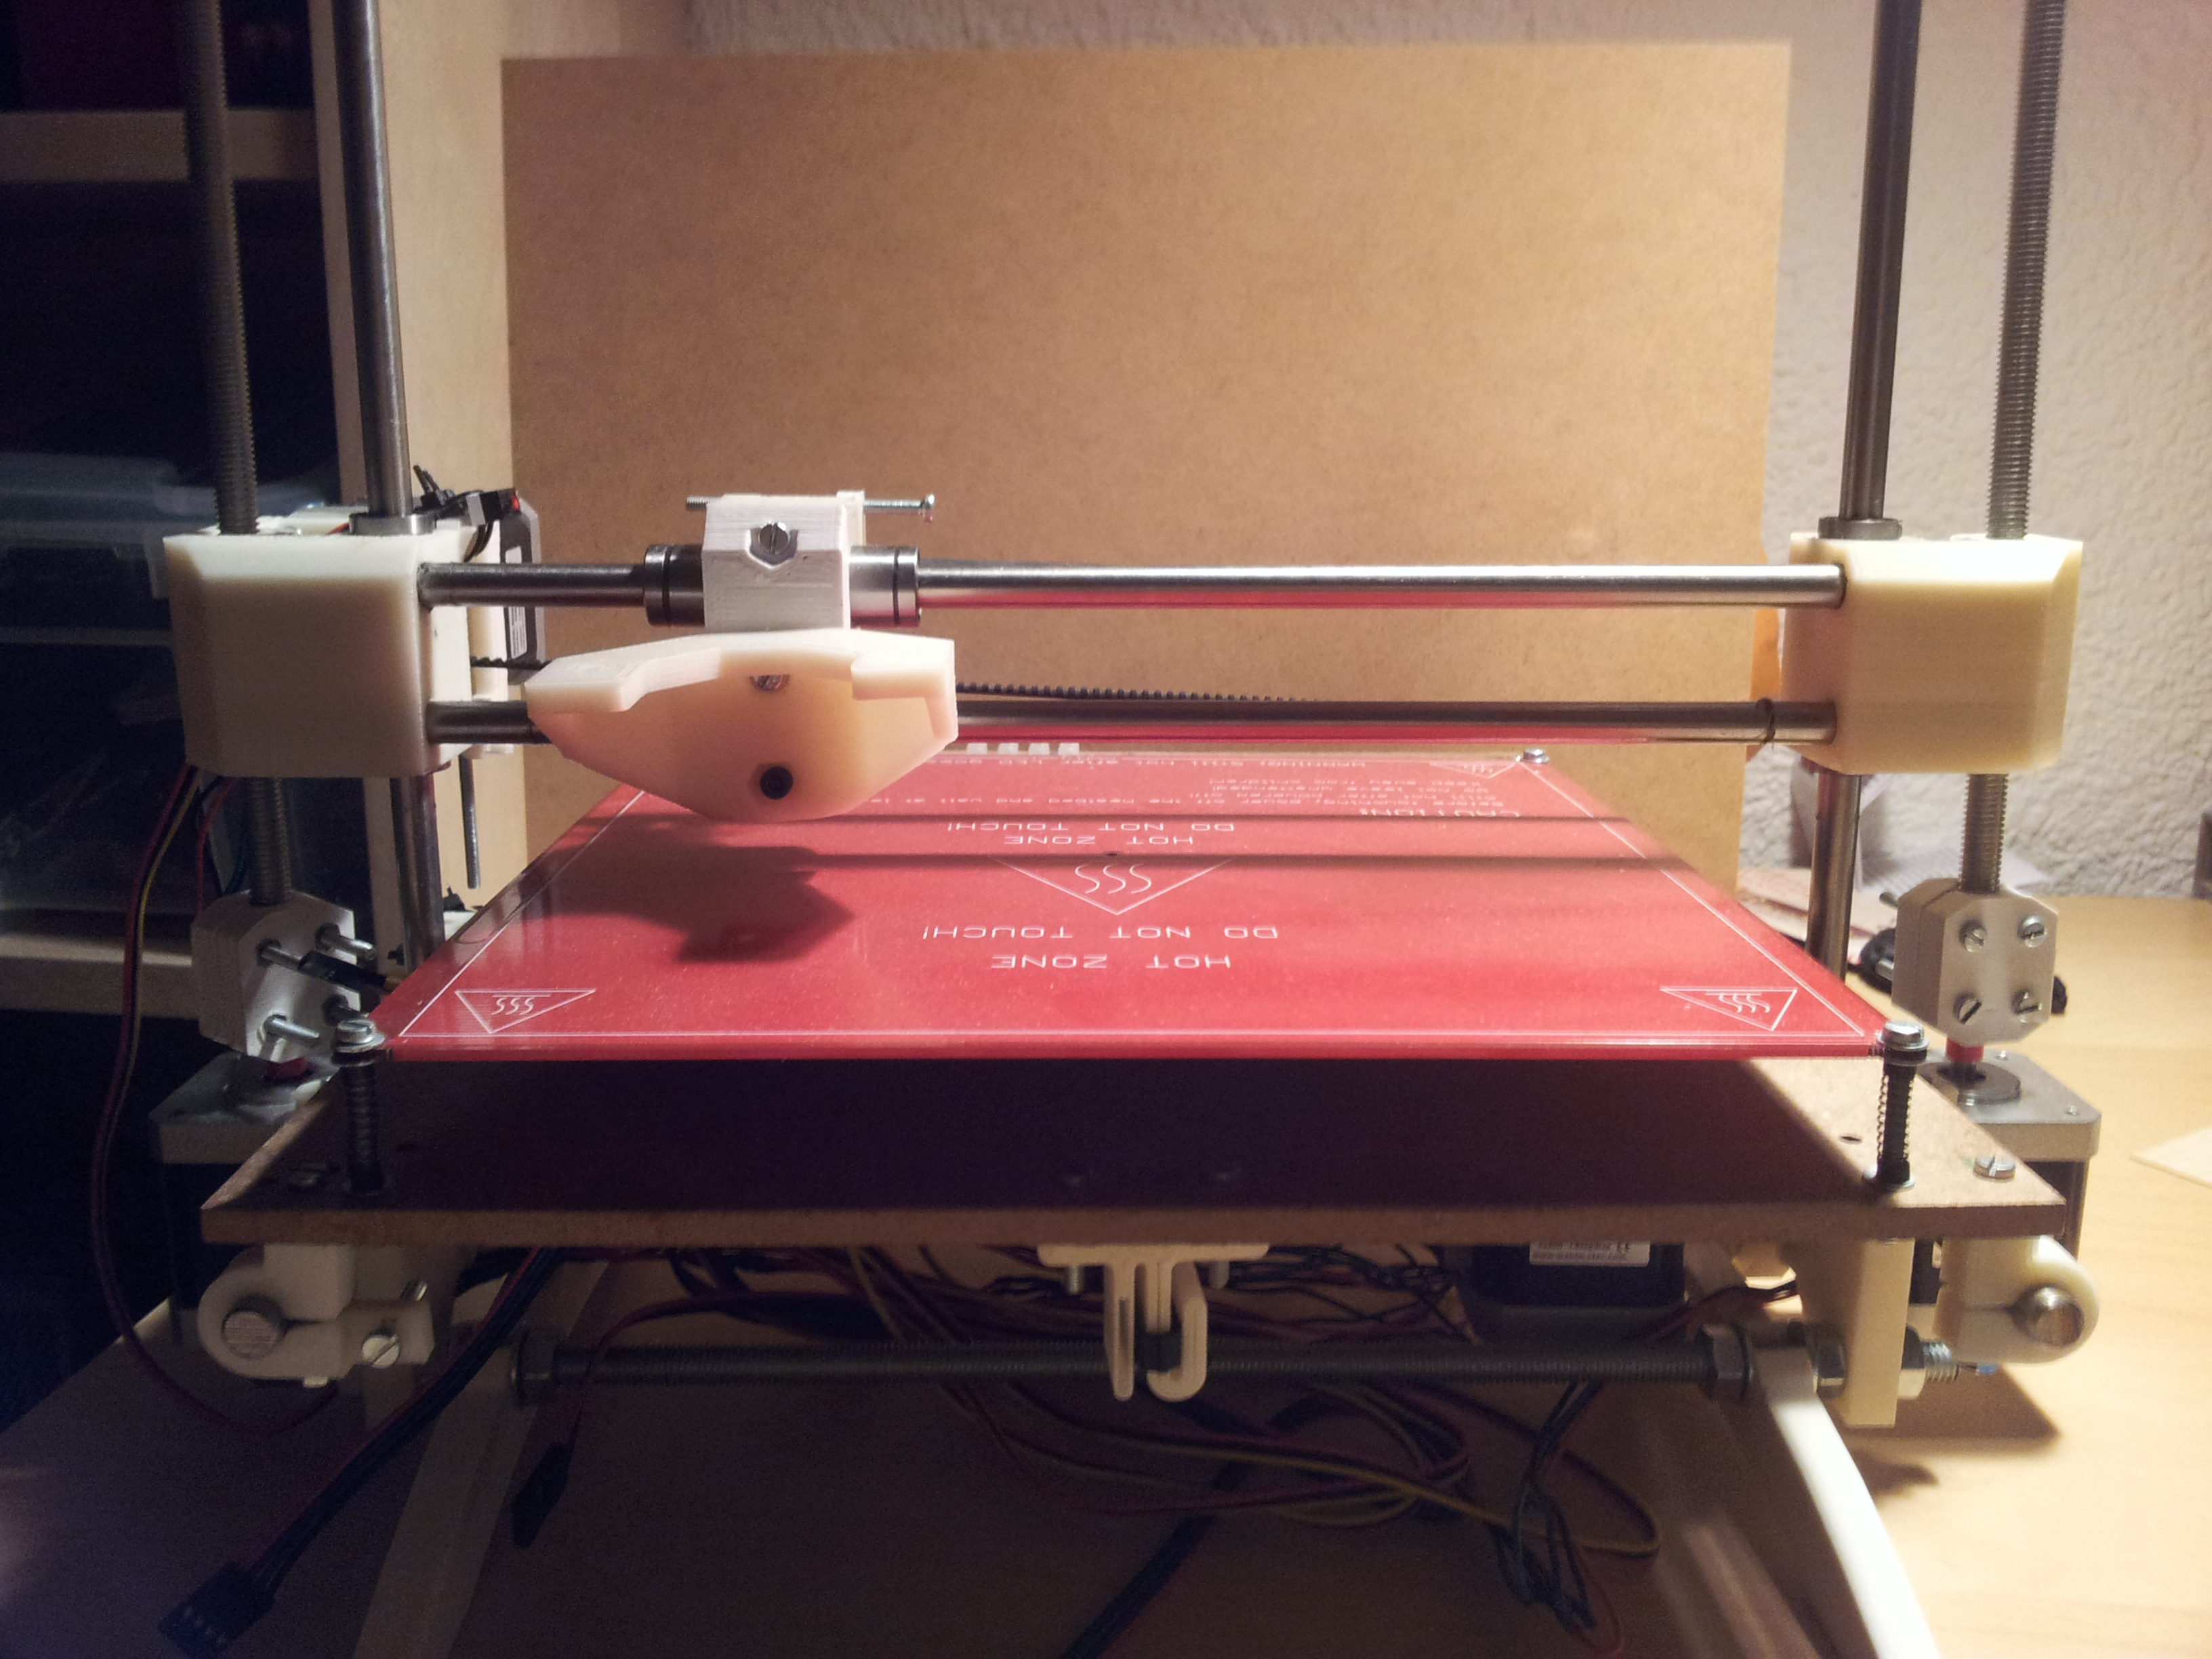
\includegraphics[width=\textwidth]{../../Fotos/94.jpg}
		                \caption{Impresora con los tres ejes montados}
		                \label{fig:23.z}
		        \end{subfigure}
		\end{figure}
		Una vez que tenemos los tres ejes montados, será el momento de nivelar  el eje Z como el la base caliente. Para ello, buscamos una superficie que esté lo suficientemente nivelada con respecto al suelo.\\
		A continuación, colocaremos un nivel entre las piezas del eje X como se muestra en la figura ~\ref{fig:25.z}. Giraremos de forma manual los lados del eje Z hasta que el nivel indique que está en nivelado.\\
		\begin{figure}[H]
		        \centering
		        \begin{subfigure}[htb]{0.5\textwidth}
		                \centering
		                \includegraphics[width=\textwidth]{../../Fotos/106.jpg}
		                \caption{Nivelando Eje Z }
		                \label{fig:25.z}
		        \end{subfigure}
		\end{figure}
		Posteriormente, comprobaremos que la pieza donde irá situado el extrusor está también nivelado( Ver foto ~\ref{fig:26.z}).
		\begin{figure}[H]
		        \centering
		        \begin{subfigure}[htb]{0.5\textwidth}
		                \centering
		                \includegraphics[width=\textwidth]{../../Fotos/107.jpg}
		                \caption{Nivelando base extrusor }
		                \label{fig:26.z}
		        \end{subfigure}
		\end{figure}
		Por último comprobaremos que la base está nivelada, en caso de no estarlo, deberemos ir apretando o aflojando los tornillos de la base. Este paso se puede hacer de forma rápida, ya que una vez que conectemos la electrónica, se deberá comprobar con el extrusor que la base está nivelada perfectamente.
		\begin{figure}[H]
		        \centering
		        \begin{subfigure}[htb]{0.5\textwidth}
		                \centering
		                \includegraphics[width=\textwidth]{../../Fotos/108.jpg}
		                \caption{Nivelando base extrusor }
		                \label{fig:27.z}
		        \end{subfigure}
		\end{figure}
